\documentclass[a4paper,12pt]{report}

\usepackage[T1]{fontenc}
\usepackage[utf8]{vietnam}
\usepackage[vietnamese]{babel}

\usepackage{tgtermes}
% ===== Math =====
\usepackage{amsmath, amssymb, amsfonts, amsthm}
\usepackage{gensymb, textcomp}

% ===== Table & Layout =====
\usepackage{array, tabularx, longtable, booktabs, multirow, multicol}
\usepackage{siunitx}
\usepackage{diagbox}

% ===== Graphic =====
\usepackage{graphicx}
\usepackage{subcaption}
\usepackage{float}
\usepackage{rotating}
\usepackage{adjustbox}

% ===== Text & Format =====
\usepackage{setspace}
\usepackage{indentfirst}
\usepackage{ragged2e}
\usepackage{lmodern}
\usepackage{titlesec}
\usepackage{enumitem}



% ===== Code =====
\usepackage{listings}
\usepackage{matlab-prettifier}

% ===== Color =====
\usepackage[dvipsnames]{xcolor}

% ===== Drawing =====
\usepackage{tikz, tkz-tab}
\usetikzlibrary{shapes.geometric, arrows}

% ===== Box =====
\usepackage{mdframed}
\usepackage{framed}
\usepackage{tcolorbox}
\tcbuselibrary{minted,breakable,xparse,skins}

% ===== System =====
\usepackage{etoolbox}
\usepackage{scrextend}
\usepackage{xurl}

% ===== Algorithm =====
\usepackage{algorithm2e}

% ===== Hyperlink =====
\usepackage[
    colorlinks=true,
    linkcolor=black,
    urlcolor=blue,
    citecolor=blue
]{hyperref}

% ===== Geometry =====
\usepackage[
    left=2.3cm,
    right=2cm,
    top=2.5cm,
    bottom=2.5cm,
    bindingoffset=1cm
]{geometry}

% ===== Header/Footer =====
\usepackage{fancyhdr}
\usepackage{lastpage}

% ===== Minted =====
\usepackage{minted}

% ===== Custom =====
\definecolor{light-gray}{gray}{0.95}
\definecolor{codegreen}{rgb}{0,0.6,0}
\definecolor{codegray}{rgb}{0.5,0.5,0.5}
\definecolor{codepurple}{rgb}{0.58,0,0.82}
\definecolor{backcolour}{rgb}{0.95,0.95,0.92}

\newcommand{\code}[1]{\colorbox{light-gray}{\texttt{#1}}}

% ===== Fancy Header =====
\usepackage{xcolor}
\definecolor{bkblue}{RGB}{0,102,204}
\definecolor{bkgray}{RGB}{80,80,80}
\definecolor{chaptercolor}{RGB}{0,102,204}

\pagestyle{fancy}
\fancyhf{}

\fancyhead[L]{
 \begin{tabular}{rl}
    \begin{picture}(15,15)(0,0)
    \put(0,-8){
\includegraphics[width=9mm]{image/LogoBK.png}}
   \end{picture}&
	\begin{tabular}{l}
		 {\color{bkblue}\bfseries\small Trường Đại học Bách Khoa TP.HCM}\\[-0.3ex]
         {\color{bkgray}\small Khoa Khoa học và Kỹ thuật Máy tính}
	\end{tabular} 
 \end{tabular}
}

\fancyfoot[L]{\footnotesize \itshape Đồ án Kỹ thuật Máy tính}
\fancyfoot[R]{\footnotesize Trang \thepage/\pageref{LastPage}}

\renewcommand{\footrulewidth}{0.5pt}





\titleformat{\chapter}[display]
  {\normalfont\bfseries\Huge\color{chaptercolor}}
  {\filleft\Huge\chaptername\ \thechapter}
  {2ex}
  {\titlerule\vspace{2ex}\filright}
  [\vspace{2ex}\titlerule]

% ===== Caption =====
\usepackage{caption}
\captionsetup{labelfont={bf}}

% ===== Section format =====
\titleformat{\paragraph}
{\normalfont\normalsize\itshape}{\theparagraph}{1em}{}
\titlespacing*{\paragraph}{0pt}{3.25ex}{1.5ex}

% ===== Custom label =====
\makeatletter
\newcommand{\mylabel}[2]{#2\def\@currentlabel{#2}\label{#1}}
\makeatother

\titlespacing*{\section}
{0pt}{0.5em}{1em}

\begin{document}

\setstretch{1.3}

% ===== COVER =====
\begin{titlepage}
%     \begin{tikzpicture}[remember picture,overlay,inner sep=0,outer sep=0]
%          \draw[blue!70!black,line width=4pt] ([xshift=-1.5cm,yshift=-2cm]current page.north east) coordinate (A)--([xshift=2.8cm,yshift=-2cm]current page.north west) coordinate(B)--([xshift=2.8cm,yshift=2cm]current page.south west) coordinate (C)--([xshift=-1.5cm,yshift=2cm]current page.south east) coordinate(D)--cycle;
    
%          \draw ([yshift=0.5cm,xshift=-0.5cm]A)-- ([yshift=0.5cm,xshift=0.5cm]B)--
%          ([yshift=-0.5cm,xshift=0.5cm]B) --([yshift=-0.5cm,xshift=-0.5cm]B)--([yshift=0.5cm,xshift=-0.5cm]C)--([yshift=0.5cm,xshift=0.5cm]C)--([yshift=-0.5cm,xshift=0.5cm]C)-- ([yshift=-0.5cm,xshift=-0.5cm]D)--([yshift=0.5cm,xshift=-0.5cm]D)--([yshift=0.5cm,xshift=0.5cm]D)--([yshift=-0.5cm,xshift=0.5cm]A)--([yshift=-0.5cm,xshift=-0.5cm]A)--([yshift=0.5cm,xshift=-0.5cm]A);
    
    
%          \draw ([yshift=-0.3cm,xshift=0.3cm]A)-- ([yshift=-0.3cm,xshift=-0.3cm]B)--
%          ([yshift=0.3cm,xshift=-0.3cm]B) --([yshift=0.3cm,xshift=0.3cm]B)--([yshift=-0.3cm,xshift=0.3cm]C)--([yshift=-0.3cm,xshift=-0.3cm]C)--([yshift=0.3cm,xshift=-0.3cm]C)-- ([yshift=0.3cm,xshift=0.3cm]D)--([yshift=-0.3cm,xshift=0.3cm]D)--([yshift=-0.3cm,xshift=-0.3cm]D)--([yshift=0.3cm,xshift=-0.3cm]A)--([yshift=0.3cm,xshift=0.3cm]A)--([yshift=-0.3cm,xshift=0.3cm]A);
%     \end{tikzpicture}
\begin{tikzpicture}[remember picture,overlay]
    \draw[
        black,
        line width=5pt
    ]
    ([xshift=2cm,yshift=-2cm]current page.north west)
    rectangle
    ([xshift=-1cm,yshift=2cm]current page.south east);
\end{tikzpicture}    
    \begin{center}
        \vspace{-10pt}
        {\Large \textbf{ĐẠI HỌC QUỐC GIA TP.HCM}}\\[0.2cm]
{\Large \textbf{TRƯỜNG ĐẠI HỌC BÁCH KHOA TP.HCM}}\\[0.2cm]
{\Large \textbf{KHOA KHOA HỌC \& KỸ THUẬT MÁY TÍNH}}\\
        \vspace{30pt}
        
\includegraphics[width=0.25\linewidth]{image/LogoBK.png}\\
        \vspace{40pt}
        \textbf{\LARGE\textbf{LUẬN VĂN TỐT NGHIỆP}}\\
        \vspace{10pt}
        \hrule
        \vspace{16pt}
        \textcolor{blue}{\Large{\textbf{PHÁT TRIỂN NỀN TẢNG NHÚNG ĐA CHỨC NĂNG DỰA TRÊN YOCTO PROJECT CHO CÁC ỨNG DỤNG TỰ ĐỘNG HÓA TRONG CÔNG NGHIỆP}}}\\
        \vspace{16pt}
        \hrule
    \end{center}
    
    \begin{center}
        \large{\textbf{HK252}}\\
        \textbf{Giảng viên hướng dẫn: TS.Lê Trọng Nhân}
    \end{center}
    
    \begin{adjustbox}{width=0.94\textwidth,center=\textwidth}
        \small
        \begin{tabular}{|>{\centering\arraybackslash}m{1cm}|>{\centering\arraybackslash}m{4.5cm}|>{\centering\arraybackslash}m{1.7cm}|>{\centering\arraybackslash}m{2.5cm}|>{\centering\arraybackslash}m{2cm}|}
            \hline
            \textbf{STT} & \textbf{Họ \& Tên} & \textbf{MSSV} & \textbf{Lớp} & \textbf{Đánh giá}\\
            \hline
                1& Đỗ Tuấn Anh & 2210050 & MT22KT01 & 100\% \\
                2& Dương Minh Hiếu & 2210978 & MT22KT01 & 100\% \\
                3& Nguyễn Hạo Duy & 2210512 & MT22KT01 & 100\% \\
            \hline
        \end{tabular}
    \end{adjustbox}
    \vspace{80pt}
    \begin{center}

        \textit{TP.Hồ Chí Minh, tháng 5 năm 2025}
    \end{center}

\end{titlepage}
\newpage

% ===== THÔNG TIN HỘI ĐỒNG =====

\section*{\centering Lời cam đoan}
Nhóm tác giả xin cam đoan rằng nhóm đã hoàn toàn thực hiện đồ án chuyên ngành này,
dưới sự hướng dẫn của TS. Lê Trọng Nhân, Khoa Khoa Học và Kỹ Thuật Máy Tính,
Trường Đại học Bách Khoa - Đại học Quốc gia. Kết quả nghiên cứu của nhóm chưa
được công bố dưới bất kỳ hình thức nào trước đó.

Tất cả các tài liệu được sử dụng trong đồ án này được thu thập từ nhiều hệ thống và
nguồn tham khảo khác nhau. Các tài liệu này đều được trích dẫn đầy đủ trong phần tài
liệu tham khảo.

Nếu có bất kỳ trường hợp đạo văn nào, nhóm xin chịu mọi trách nhiệm. Đại học Quốc
gia Thành phố Hồ Chí Minh sẽ không chịu trách nhiệm về bất kỳ vi phạm bản quyền
nào xảy ra trong quá trình nghiên cứu của nhóm.

\begin{flushright}
TP. Hồ Chí Minh, tháng 5 năm 2026 \\
Sinh viên thực hiện \\
Dương Minh Hiếu \\
Đỗ Tuấn Anh \\ 
Nguyễn Hạo Duy \\
\end{flushright}
\newpage

% ===== LỜI CẢM ƠN =====
\section*{\centering Lời cảm ơn}

Để hoàn thành khóa luận tốt nghiệp này, em đã nhận được rất nhiều sự hỗ trợ,
động viên và giúp đỡ quý báu từ quý Thầy Cô, gia đình, bạn bè và những người
đã đồng hành cùng em trong suốt quá trình học tập và nghiên cứu. Em xin được
gửi lời cảm ơn chân thành đến tất cả mọi người.

Trước hết, em xin trân trọng cảm ơn Ban Giám hiệu cùng quý Thầy Cô Trường
Đại học Bách khoa – Đại học Quốc gia Thành phố Hồ Chí Minh nói chung và
quý Thầy Cô thuộc Khoa Khoa học và Kỹ thuật Máy tính nói riêng. Những kiến
thức chuyên môn, phương pháp tư duy và tinh thần học tập nghiêm túc mà quý
Thầy Cô truyền đạt trong suốt thời gian qua là nền tảng quan trọng giúp em có
thể thực hiện và hoàn thành khóa luận này.

Em xin bày tỏ lòng biết ơn sâu sắc và chân thành nhất đến Thầy Lê Trọng Nhân,
người đã trực tiếp hướng dẫn và đồng hành cùng em trong quá trình thực hiện đề
tài ``Phát triển nền tảng nhúng đa chức năng dựa trên Yocto Project cho các ứng
dụng tự động hóa trong công nghiệp''. Thầy không chỉ tận tình định hướng nội
dung nghiên cứu mà còn luôn hỗ trợ, góp ý và chia sẻ nhiều kinh nghiệm quý báu
trong quá trình triển khai hệ thống Linux Embedded, Yocto Project và phát triển
Kernel Driver. Những kiến thức và kinh nghiệm mà Thầy truyền đạt là hành trang
quan trọng giúp em hoàn thiện đề tài cũng như định hướng cho công việc và quá
trình nghiên cứu sau này.

Em cũng xin gửi lời cảm ơn đến các anh chị, bạn bè đã luôn hỗ trợ, trao đổi kiến
thức và chia sẻ kinh nghiệm trong suốt quá trình thực hiện khóa luận. Những sự
động viên và giúp đỡ đó đã giúp em có thêm động lực để vượt qua những khó
khăn trong quá trình nghiên cứu và phát triển hệ thống.

Cuối cùng, em xin gửi lời tri ân sâu sắc đến gia đình và người thân, những người
đã luôn bên cạnh động viên, ủng hộ và tạo điều kiện tốt nhất để em có thể yên
tâm học tập và hoàn thành khóa luận tốt nghiệp này.

Mặc dù đã cố gắng hoàn thiện khóa luận một cách tốt nhất, tuy nhiên do hạn chế
về thời gian, kiến thức và kinh nghiệm thực tế, khóa luận khó tránh khỏi những
thiếu sót nhất định. Em rất mong nhận được những ý kiến đóng góp quý báu từ
quý Thầy Cô để đề tài được hoàn thiện hơn.

\vspace{1cm}

\begin{flushright}
TP. Hồ Chí Minh, tháng 5 năm 2026 \\
Sinh viên thực hiện
\end{flushright}
\newpage

% ===== TÓM TẮT =====
% \input{sections/abstract}

% ===== MỤC LỤC =====
\renewcommand{\contentsname}{Mục Lục}
\tableofcontents
\newpage

% ===== DANH SÁCH =====
\renewcommand{\listtablename}{Danh sách bảng}
\listoftables
\newpage

\renewcommand{\listfigurename}{Danh sách hình}
\listoffigures
\newpage

% ===== MỞ ĐẦU =====
\chapter{Phần mở đầu}
\begin{enumerate}[
    leftmargin=2.5em,
    labelsep=0.8em,
    itemsep=0.6em
]
  \renewcommand{\labelenumi}{\textcolor{chaptercolor}{\bfseries \thechapter.\arabic{enumi}}}

  \item \textbf{Đặt vấn đề}
  \item \textbf{Lý do chọn đề tài}
  \item \textbf{Mục tiêu nghiên cứu}
  \item \textbf{Phạm vi và giới hạn nghiên cứu}
  \item \textbf{Bố cục luận văn}
\end{enumerate}
\newpage
\section{Đặt vấn đề}

Trong bối cảnh chuyển đổi số và sự phát triển mạnh mẽ của cuộc cách mạng công nghiệp 4.0, các hệ thống nhúng và Internet of Things (IoT) đang ngày càng được ứng dụng rộng rãi trong nhiều lĩnh vực như sản xuất thông minh, giám sát môi trường, quản lý năng lượng và tự động hóa công nghiệp. Các hệ thống này không chỉ yêu cầu khả năng thu thập và xử lý dữ liệu theo thời gian thực mà còn đòi hỏi tính ổn định, khả năng mở rộng và mức độ bảo mật cao trong suốt quá trình vận hành.

Tuy nhiên, nhiều nền tảng nhúng hiện nay vẫn phụ thuộc vào các giải pháp đóng hoặc thiếu khả năng tùy biến sâu theo yêu cầu thực tế của từng hệ thống. Đối với các thiết bị biên (Edge Device), việc tối ưu tài nguyên phần cứng, kiểm soát thành phần phần mềm và đảm bảo khả năng vận hành ổn định là những yêu cầu đặc biệt quan trọng. Bên cạnh đó, sự gia tăng của các nguy cơ tấn công mạng, giả mạo firmware hoặc thay đổi dữ liệu trái phép cũng đặt ra yêu cầu cần có các cơ chế bảo vệ tính toàn vẹn và bảo mật cho hệ thống nhúng.

Trong lĩnh vực quản lý kho và giám sát môi trường công nghiệp, việc theo dõi các thông số như nhiệt độ, độ ẩm và trạng thái vận hành đóng vai trò quan trọng nhằm đảm bảo chất lượng lưu trữ hàng hóa, lương thực và thực phẩm. Các hệ thống giám sát truyền thống thường tồn tại nhiều hạn chế như khả năng mở rộng thấp, khó tùy biến hoặc phụ thuộc vào nền tảng phần mềm riêng biệt. Do đó, việc nghiên cứu và xây dựng một nền tảng Linux Embedded có khả năng tùy biến, hỗ trợ giao tiếp IoT và tích hợp các cơ chế bảo mật là cần thiết nhằm đáp ứng nhu cầu thực tế của các hệ thống công nghiệp hiện đại.

\begin{figure}[H]
    \centering
    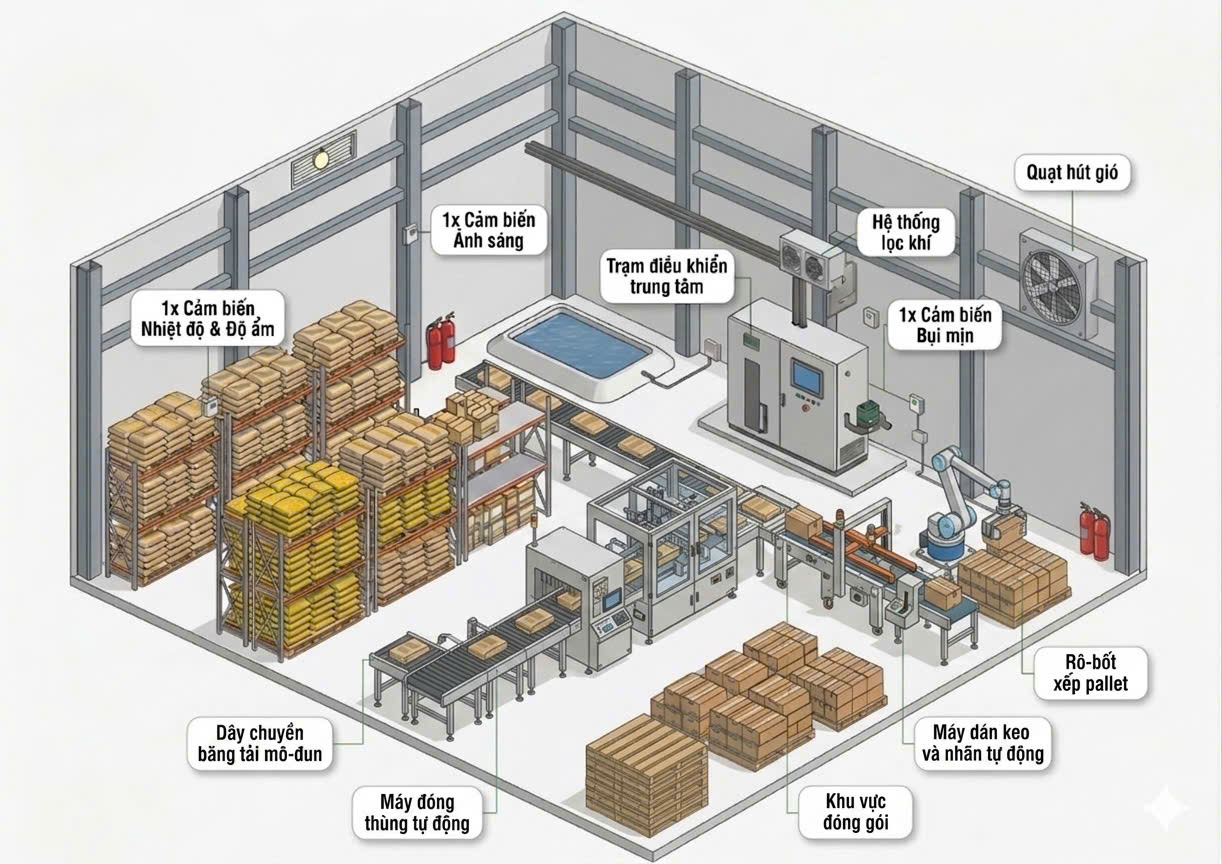
\includegraphics[width=0.8\linewidth]{image/baitoan.jpg}
    \caption{Mô hình bài toán đặt ra}
    \label{fig:placeholder}
\end{figure}

\section{Lý do chọn đề tài}

Yocto Project là nền tảng mã nguồn mở mạnh mẽ cho phép xây dựng và tùy biến hệ điều hành Linux nhúng theo từng kiến trúc phần cứng và yêu cầu ứng dụng cụ thể. Khác với các bản phân phối Linux truyền thống, Yocto cung cấp khả năng kiểm soát chi tiết các thành phần hệ thống, tối ưu tài nguyên và chủ động trong quá trình phát triển Embedded Linux Image.\cite{yocto_project_overview}

Bên cạnh khả năng tùy biến hệ thống, Yocto Project còn hỗ trợ tích hợp nhiều cơ chế bảo mật hiện đại như Secure Boot, dm-verity và fscrypt nhằm tăng cường tính toàn vẹn và độ an toàn cho hệ thống nhúng. Đây là những yếu tố đặc biệt quan trọng trong các hệ thống công nghiệp và IoT, nơi thiết bị thường hoạt động liên tục trong thời gian dài và yêu cầu độ ổn định cao.

Ngoài ra, việc phát triển các Linux Device Driver và tích hợp giao tiếp phần cứng trong môi trường Yocto cũng giúp tăng khả năng làm chủ hệ thống ở mức thấp, đồng thời tạo điều kiện thuận lợi cho việc nghiên cứu kiến trúc Linux Embedded một cách toàn diện hơn.

Xuất phát từ những yêu cầu thực tế trong lĩnh vực IoT và tự động hóa công nghiệp, đề tài được thực hiện nhằm nghiên cứu và xây dựng một nền tảng nhúng đa chức năng dựa trên Yocto Project, có khả năng tích hợp các cơ chế bảo mật, hỗ trợ giao tiếp thiết bị và phục vụ triển khai các ứng dụng giám sát công nghiệp. Trên cơ sở đó, đề tài triển khai bài toán giám sát kho thông minh như một mô hình ứng dụng thực tế để đánh giá tính ổn định, khả năng mở rộng và hiệu quả vận hành của hệ thống.

\begin{figure}[H]
    \centering
    
\includegraphics[width=0.5\linewidth]{image/yoctoc1.png}
    \caption{Nền tảng Yocto Project}
    \label{fig:placeholder}
\end{figure}

\section{Mục tiêu nghiên cứu}

Đề tài hướng đến mục tiêu nghiên cứu và xây dựng nền tảng Linux Embedded phục vụ cho các ứng dụng công nghiệp và IoT dựa trên Yocto Project. Hệ thống được thiết kế theo hướng tùy biến, có khả năng mở rộng và đáp ứng yêu cầu vận hành ổn định trên các thiết bị nhúng tài nguyên hạn chế.

Bên cạnh đó, đề tài tập trung nghiên cứu cơ chế xây dựng và tích hợp Linux Device Driver nhằm hỗ trợ giao tiếp phần cứng trong hệ thống nhúng. Các cơ chế quản lý module, Device Tree và tích hợp driver trong Yocto cũng được nghiên cứu nhằm xây dựng nền tảng phát triển Embedded Linux hoàn chỉnh hơn.

Ngoài khả năng vận hành hệ thống, đề tài còn nghiên cứu và tích hợp các cơ chế bảo mật nhằm đảm bảo tính toàn vẹn của firmware, filesystem và dữ liệu thiết bị. Đồng thời, hệ thống hỗ trợ cơ chế giao tiếp IoT thông qua các giao thức như MQTT và HTTP nhằm phục vụ việc giám sát và truyền dữ liệu theo thời gian thực.

Trên cơ sở nền tảng được xây dựng, đề tài triển khai mô hình quản lý kho thông minh nhằm kiểm chứng khả năng ứng dụng thực tế của hệ thống trong việc giám sát môi trường kho, thu thập dữ liệu cảm biến, cảnh báo trạng thái bất thường và quản lý thiết bị từ xa.

\begin{figure}[H]
    \centering
    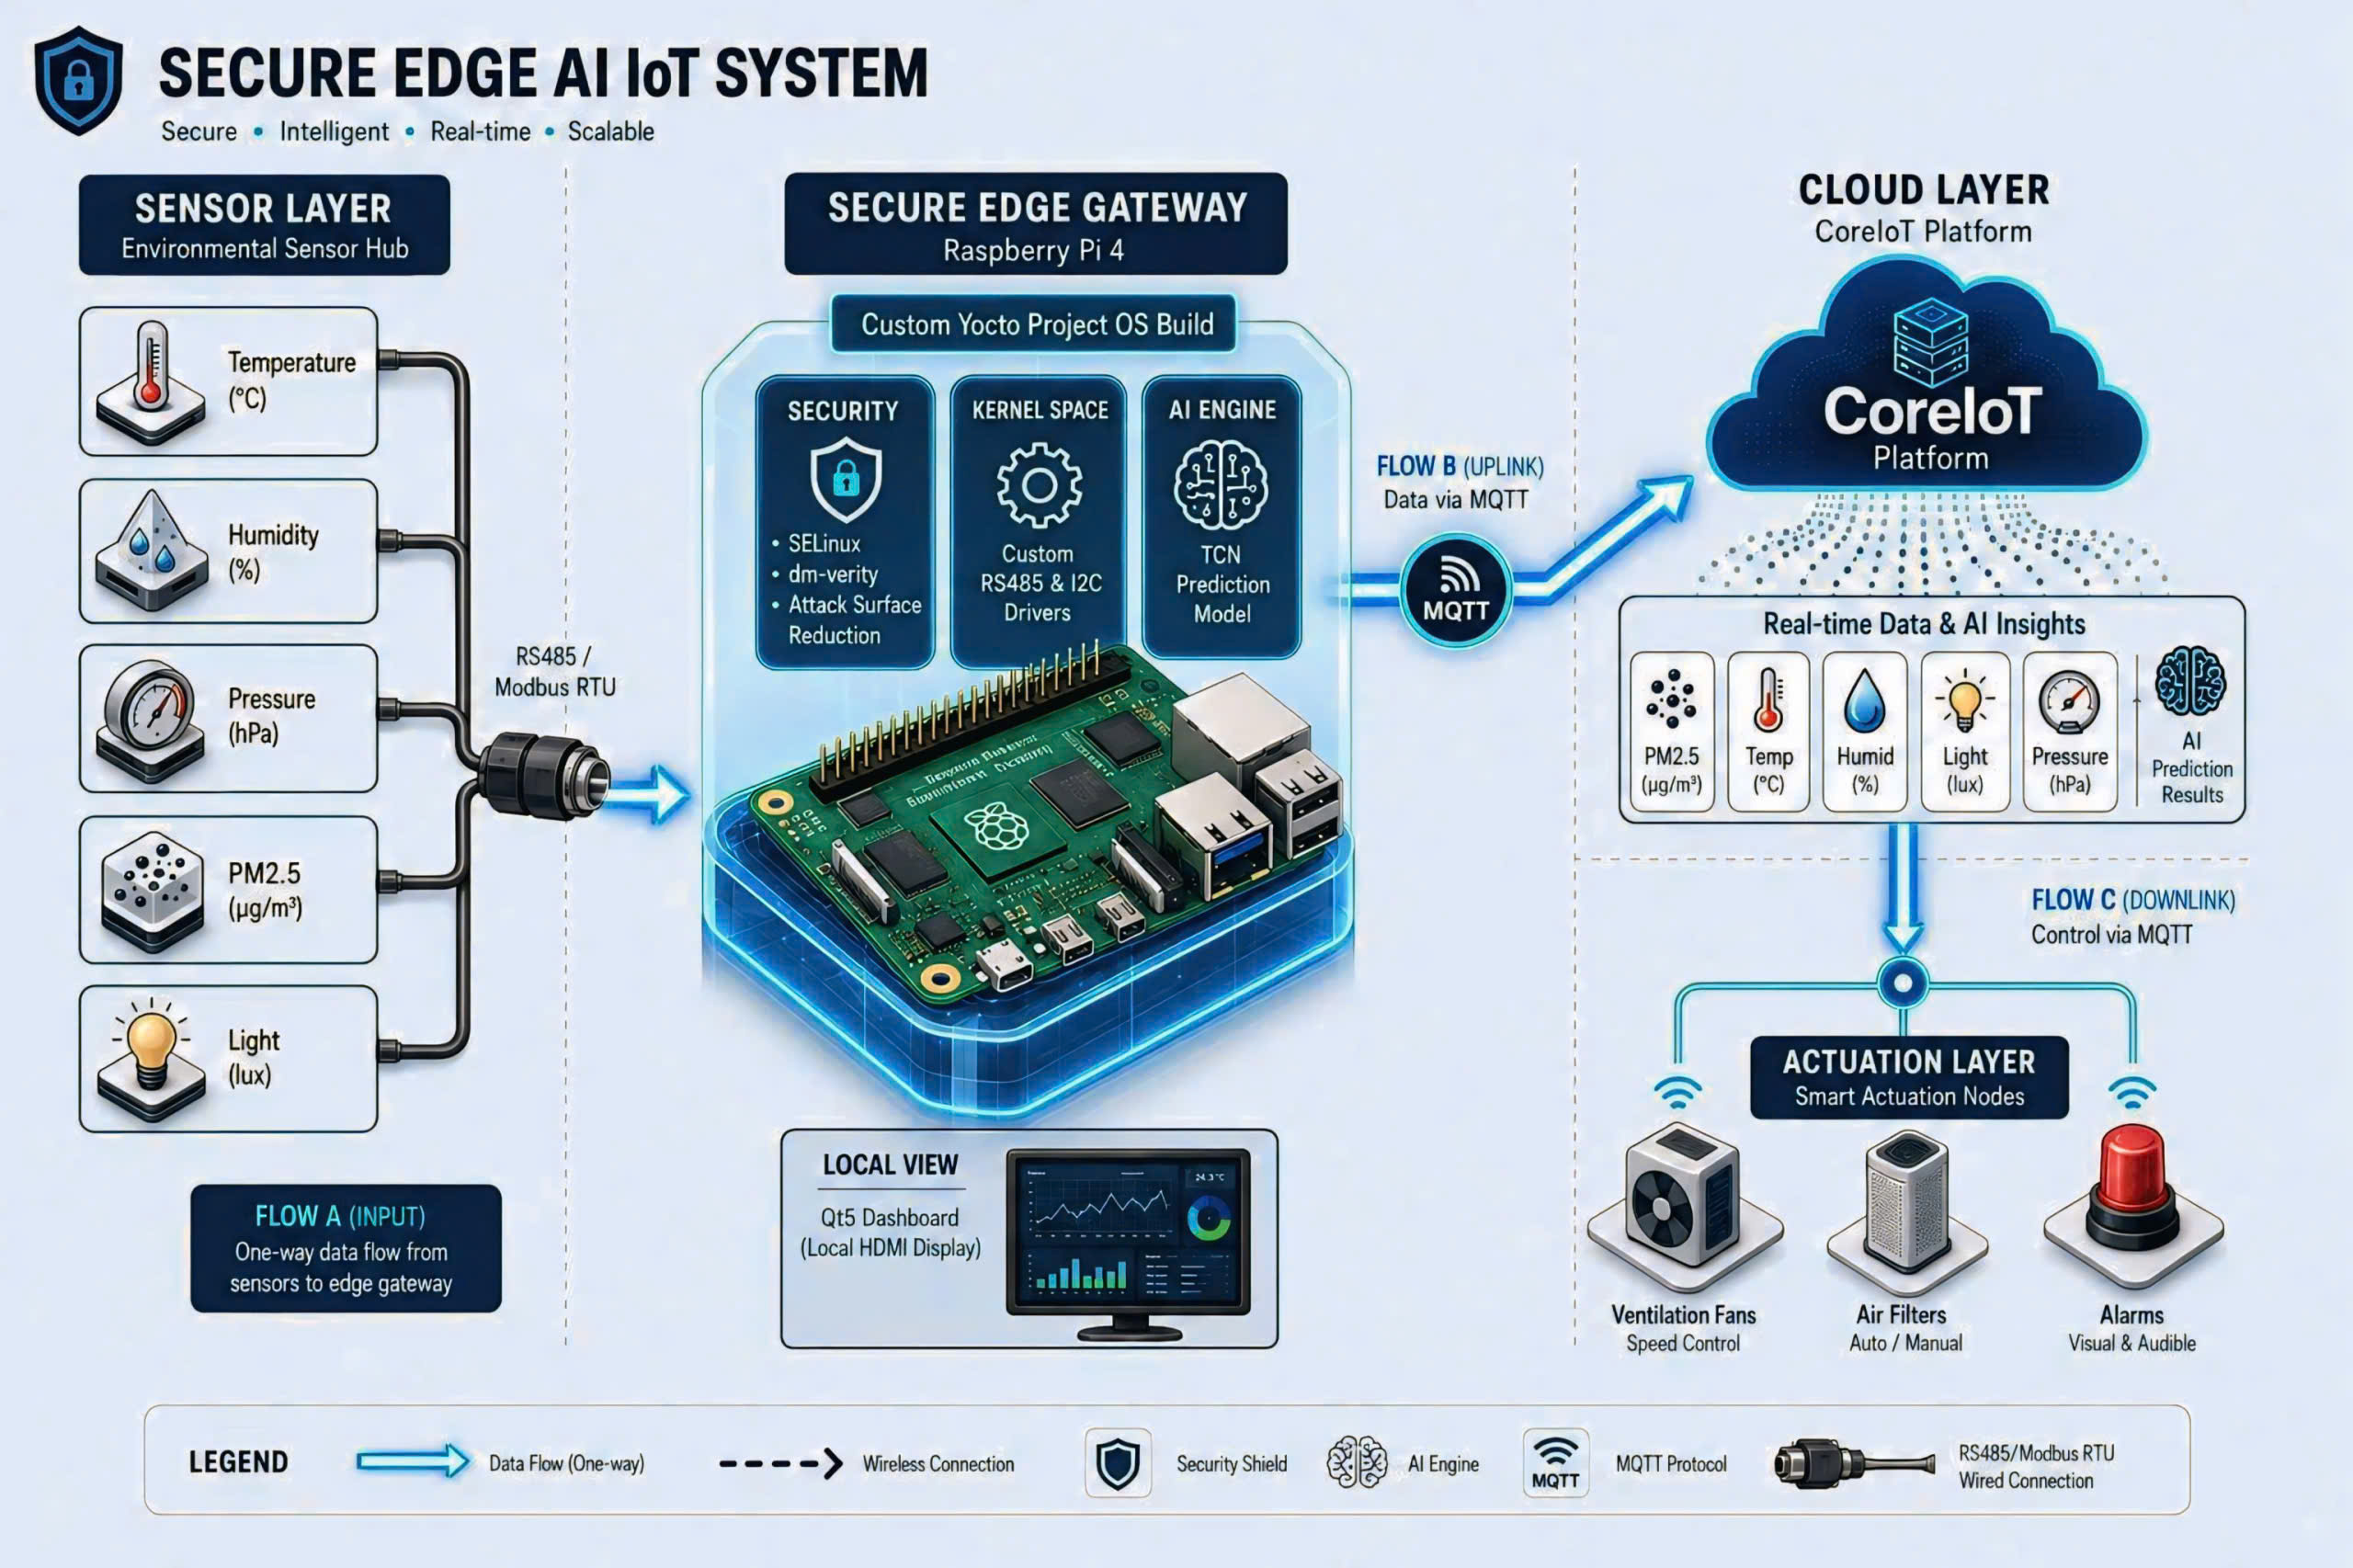
\includegraphics[width=0.9\linewidth]{image/kientructongquan.jpg}
    \caption{Kiến trúc tổng thể của hệ thống}
    \label{fig:placeholder}
\end{figure}

\section{Phạm vi và giới hạn nghiên cứu}

Đề tài tập trung xây dựng nền tảng Linux nhúng (Embedded Linux) dành cho các ứng dụng công nghiệp và IoT (Internet of Things) dựa trên Yocto Project. Hệ điều hành được phát triển theo hướng tùy biến cao, phù hợp với thiết bị biên (Edge Device) có tài nguyên phần cứng giới hạn. Trên cơ sở đó, nội dung nghiên cứu bao gồm cơ chế build image, quản lý gói phần mềm (package) và tích hợp Linux Device Driver trong môi trường Yocto nhằm đáp ứng yêu cầu giao tiếp, điều khiển phần cứng trên hệ thống nhúng.

Bên cạnh việc phát triển nền tảng, đề tài còn đi sâu vào các thành phần cốt lõi của Linux Kernel như Kernel Module, Device Tree và cơ chế quản lý module lúc runtime. Những kiến thức này là nền tảng cho việc phát triển và tích hợp driver trong hệ thống Linux nhúng, đồng thời nâng cao khả năng làm chủ hệ thống ở mức thấp đối với các bài toán công nghiệp.

Về mặt bảo mật, đề tài tích hợp một số cơ chế phổ biến trong Linux Embedded như Secure Boot, dm-verity và fscrypt nhằm tăng cường bảo vệ firmware, filesystem và dữ liệu trên thiết bị. Hệ thống cũng hỗ trợ các chức năng quản lý dịch vụ và cấu hình cơ bản để đảm bảo vận hành ổn định trong thực tế.

Về truyền thông và IoT, nền tảng triển khai cơ chế kết nối giữa thiết bị và hệ thống quản lý qua các giao thức MQTT và HTTP. Hệ thống có khả năng thu thập, xử lý và truyền dữ liệu cảm biến theo thời gian thực, đồng thời xây dựng cơ chế giám sát và cảnh báo phục vụ quản lý thiết bị trong môi trường công nghiệp.

Để kiểm chứng khả năng ứng dụng thực tế, đề tài triển khai mô hình quản lý kho thông minh dựa trên nền tảng đã xây dựng. Mô hình này tập trung giám sát các thông số môi trường như nhiệt độ, độ ẩm và trạng thái hoạt động của kho hàng, kèm theo dashboard giám sát và backend cơ bản để lưu trữ, hiển thị và quản lý dữ liệu thiết bị.

Tuy nhiên, do giới hạn về thời gian, tài nguyên và phạm vi nghiên cứu, đề tài mới chỉ dừng lại ở mô hình thử nghiệm, chưa được đánh giá trên quy mô công nghiệp lớn. Các bài toán chuyên sâu như tối ưu logistics, quản lý chuỗi cung ứng hay tích hợp hệ thống ERP/WMS hoàn chỉnh chưa được đề cập. Ngoài ra, đề tài chưa nghiên cứu các cơ chế bảo mật phần cứng nâng cao (TPM, HSM) hoặc giải pháp chống tấn công vật lý. Các kỹ thuật trí tuệ nhân tạo và machine learning phục vụ dự đoán, tối ưu vận hành hệ thống cũng chưa được tích hợp trong phạm vi hiện tại.

\section{Bố cục luận văn}

Luận văn được tổ chức thành 6 chương với nội dung chính như sau:

\begin{itemize}

    \item \textbf{Chương 1: Phần mở đầu} \\ 
    Trình bày bối cảnh nghiên cứu, lý do chọn đề tài, mục tiêu nghiên cứu, phạm vi triển khai và bố cục tổng thể của luận văn.

    \item \textbf{Chương 2: Tổng quan dự án} \\ 
    Trình bày tổng quan về Linux Embedded, Yocto Project, Industrial IoT và các công nghệ liên quan đến hệ thống nhúng và tự động hóa công nghiệp.

    \item \textbf{Chương 3: Cơ sở lý thuyết} \\ 
    Trình bày các cơ sở lý thuyết phục vụ cho việc xây dựng hệ thống, bao gồm Yocto Project, BitBake, Linux Kernel, Linux Device Driver, Kernel Module và các cơ chế tích hợp driver trong Linux Embedded.

    \item \textbf{Chương 4: Thiết kế hệ thống} \\ 
    Phân tích yêu cầu hệ thống, xây dựng kiến trúc tổng thể và thiết kế các thành phần kỹ thuật như Linux Embedded Platform, Driver phần cứng, bảo mật hệ thống và cơ chế giao tiếp IoT.

    \item \textbf{Chương 5: Triển khai và đánh giá} \\ 
    Trình bày quá trình triển khai hệ điều hành bằng Yocto Project, xây dựng Linux Device Driver, tích hợp MQTT/HTTP, triển khai hệ thống giám sát và đánh giá kết quả hoạt động của hệ thống.

    \item \textbf{Chương 6: Kết luận và hướng phát triển} \\ 
    Tổng kết các kết quả đạt được, đánh giá ưu điểm và hạn chế của hệ thống, đồng thời đề xuất các hướng phát triển trong tương lai.

\end{itemize}
% ===== CHƯƠNG =====
\chapter{Tổng quan dự án}
\begin{enumerate}[
    leftmargin=2.5em,
    labelsep=0.8em,
    itemsep=0.6em
]
  \renewcommand{\labelenumi}{\textcolor{chaptercolor}{\bfseries \thechapter.\arabic{enumi}}}

  \item \textbf{Tổng quan về tự động hóa công nghiệp}
  \item \textbf{Tổng quan về hệ điều hành nhúng}
  \item \textbf{Tổng quan về Yocto Project}
  \item \textbf{Các công trình liên quan}
\end{enumerate}
\newpage
\section{Giao tiếp phần cứng công nghiệp}
\section{Linux Device Driver}

\subsection{Kiến trúc Layer trong Yocto}

Yocto Project sử dụng kiến trúc phân lớp (Layer Architecture) nhằm tổ chức metadata và mã nguồn theo hướng module hóa, linh hoạt và dễ mở rộng. Đây là một trong những đặc điểm quan trọng giúp Yocto trở thành nền tảng xây dựng Linux Embedded có khả năng tùy biến cao và phù hợp với nhiều kiến trúc phần cứng khác nhau.

Trong các hệ thống Linux Embedded hiện đại, số lượng package, driver, thư viện và thành phần hệ thống thường rất lớn. Nếu toàn bộ metadata và source code được lưu tập trung trong một cấu trúc duy nhất, việc quản lý dependency, cập nhật phiên bản và bảo trì hệ thống sẽ trở nên phức tạp. Do đó, Yocto áp dụng mô hình phân lớp nhằm chia nhỏ hệ thống thành các thành phần độc lập, mỗi layer đảm nhiệm một nhóm chức năng riêng biệt.

Kiến trúc phân lớp cho phép tách biệt rõ ràng giữa các thành phần hệ thống như BSP (Board Support Package), middleware, application và các package tùy chỉnh. Nhờ đó, người phát triển có thể dễ dàng bổ sung hoặc loại bỏ một chức năng mà không ảnh hưởng đến các thành phần còn lại của hệ thống. Điều này đặc biệt quan trọng trong phát triển hệ thống nhúng, nơi mỗi nền tảng phần cứng có thể yêu cầu các driver và cấu hình riêng biệt.

Ngoài khả năng module hóa, Layer Architecture còn giúp tăng tính tái sử dụng của metadata và source code. Một layer có thể được sử dụng lại trong nhiều dự án khác nhau mà không cần chỉnh sửa đáng kể. Ví dụ, các layer hỗ trợ kiến trúc phần cứng, networking hoặc multimedia có thể được tích hợp vào nhiều hệ thống Linux Embedded khác nhau thông qua cơ chế add-layer của Yocto.

Bên cạnh đó, việc phân lớp còn hỗ trợ hiệu quả cho quá trình cộng tác và phát triển nhóm. Mỗi nhóm phát triển có thể quản lý một layer riêng biệt tương ứng với chức năng của mình mà không làm ảnh hưởng trực tiếp đến hệ thống tổng thể. Điều này giúp giảm xung đột mã nguồn và nâng cao khả năng bảo trì dự án trong các hệ thống quy mô lớn.

Một ưu điểm quan trọng khác của kiến trúc phân lớp là khả năng quản lý ưu tiên metadata thông qua cơ chế layer priority. Khi nhiều layer cùng chứa recipe hoặc cấu hình cho một package, BitBake sẽ xác định layer có mức ưu tiên cao hơn để sử dụng. Cơ chế này cho phép người phát triển tùy chỉnh hoặc ghi đè hành vi của package mà không cần chỉnh sửa trực tiếp source code gốc.

Ngoài ra, Layer Architecture còn giúp Yocto Project duy trì tính mở rộng và khả năng nâng cấp hệ thống trong thời gian dài. Khi cần cập nhật phiên bản Linux Kernel, thêm driver mới hoặc tích hợp middleware khác, người phát triển chỉ cần bổ sung hoặc cập nhật layer tương ứng thay vì chỉnh sửa toàn bộ hệ thống build.

Nhờ các ưu điểm về tính module hóa, khả năng tái sử dụng, dễ bảo trì và hỗ trợ mở rộng hệ thống, kiến trúc phân lớp đã trở thành nền tảng cốt lõi trong thiết kế của Yocto Project và đóng vai trò quan trọng trong quá trình phát triển các hệ thống Linux Embedded hiện đại.
Mỗi layer có thể chứa:

\begin{itemize}
    \item Recipe (.bb)
    \item Configuration
    \item Patch
    \item Source code
\end{itemize}

\subsection{Các thành phần chính trong Layer của Yocto Project}

Trong Yocto Project, kiến trúc layer được xây dựng dựa trên cơ chế metadata nhằm tổ chức hệ thống build theo hướng module hóa và có khả năng mở rộng cao. Mỗi layer đóng vai trò như một đơn vị chức năng độc lập, có thể chứa đầy đủ các thành phần cần thiết để xây dựng phần mềm hoặc hệ thống Linux nhúng. Việc phân chia các thành phần trong layer giúp quá trình phát triển, bảo trì và tái sử dụng mã nguồn trở nên thuận tiện hơn. Các thành phần chính thường xuất hiện trong một layer bao gồm Recipe, Configuration, Patch và Source Code.

\subsubsection{Recipe (.bb)}

Recipe là thành phần cốt lõi trong Yocto Project, được sử dụng để mô tả toàn bộ quy trình xây dựng một package hoặc một thành phần phần mềm trong hệ thống nhúng. Các recipe thường có phần mở rộng \texttt{.bb} và được xử lý bởi BitBake Build Engine. Có thể xem recipe như một tập hợp metadata dùng để hướng dẫn hệ thống build thực hiện các công việc như tải mã nguồn, giải nén, biên dịch, cài đặt và đóng gói phần mềm.

Trong mỗi recipe, nhiều biến hệ thống được sử dụng để mô tả thông tin liên quan đến package. Các biến này bao gồm tên package, phiên bản, giấy phép sử dụng, dependency, vị trí source code và các task cần thực hiện trong quá trình build. Thông qua recipe, BitBake có thể tự động phân tích dependency giữa các package và xây dựng quy trình biên dịch phù hợp.

Ngoài vai trò quản lý build process, recipe còn hỗ trợ tính module hóa và tái sử dụng trong Yocto Project. Thay vì cấu hình thủ công từng bước biên dịch, người phát triển chỉ cần mô tả metadata trong recipe để hệ thống tự động thực hiện toàn bộ pipeline build. Điều này giúp giảm đáng kể độ phức tạp trong quá trình phát triển hệ thống Linux nhúng quy mô lớn.

Recipe cũng hỗ trợ kế thừa thông qua cơ chế class inheritance. Nhờ đó, nhiều package có thể sử dụng chung một tập chức năng build mà không cần lặp lại mã cấu hình. Đây là một trong những đặc điểm quan trọng giúp Yocto Project trở thành nền tảng build có tính mở rộng và bảo trì cao.

\subsubsection{Configuration}

Configuration là thành phần chịu trách nhiệm quản lý và thiết lập môi trường build trong Yocto Project. Các file cấu hình thường được lưu trong thư mục \texttt{conf/} và chứa các biến hệ thống phục vụ quá trình xây dựng Linux Embedded. Đây là thành phần quan trọng giúp xác định cách thức hoạt động của toàn bộ hệ thống build.

Thông qua configuration, người phát triển có thể thiết lập kiến trúc phần cứng mục tiêu, compiler, toolchain, package manager, loại filesystem và nhiều tham số hệ thống khác. Ngoài ra, configuration còn cho phép quản lý danh sách layer được sử dụng trong môi trường build cũng như thứ tự ưu tiên giữa các layer.

Một trong những vai trò quan trọng của configuration là hỗ trợ khả năng tùy biến hệ thống Linux nhúng. Tùy thuộc vào yêu cầu phần cứng và ứng dụng, người phát triển có thể thay đổi các thông số cấu hình để tạo ra các image Linux tối ưu về kích thước, hiệu năng hoặc mức tiêu thụ tài nguyên.

Các file configuration trong Yocto thường được tổ chức theo nhiều cấp độ khác nhau như cấu hình toàn cục, cấu hình machine, cấu hình distro hoặc cấu hình riêng cho từng layer. Nhờ kiến trúc này, Yocto Project có khả năng quản lý các hệ thống build phức tạp với số lượng package và dependency rất lớn.

Ngoài chức năng quản lý môi trường build, configuration còn đóng vai trò quan trọng trong việc đảm bảo tính tái lập của hệ thống. Khi các thông số build được định nghĩa rõ ràng trong configuration, hệ thống có thể được build lại với kết quả tương đồng trên nhiều môi trường phát triển khác nhau.

\subsubsection{Patch}

Patch là thành phần được sử dụng để sửa đổi hoặc cập nhật mã nguồn trong quá trình build mà không cần thay đổi trực tiếp source code gốc. Trong Yocto Project, patch đóng vai trò quan trọng trong việc tùy biến phần mềm, sửa lỗi hệ thống và bổ sung chức năng mới cho các package.

Patch thường được lưu dưới dạng file \texttt{.patch} hoặc \texttt{.diff}. Các file này chứa thông tin thay đổi giữa phiên bản mã nguồn gốc và phiên bản đã được chỉnh sửa. Trong quá trình build, BitBake sẽ tự động áp dụng patch trước khi thực hiện biên dịch mã nguồn.

Việc sử dụng patch mang lại nhiều lợi ích trong phát triển hệ thống nhúng. Trước hết, patch giúp duy trì tính nguyên vẹn của source code gốc, từ đó tạo thuận lợi cho việc cập nhật phiên bản mới hoặc đồng bộ với repository chính thức. Bên cạnh đó, patch còn hỗ trợ quản lý thay đổi một cách rõ ràng và có hệ thống, giúp quá trình bảo trì phần mềm trở nên dễ dàng hơn.

Trong các hệ thống Linux Embedded, patch thường được sử dụng để tối ưu kernel, sửa lỗi driver, tùy biến bootloader hoặc bổ sung hỗ trợ cho phần cứng mới. Đây là kỹ thuật phổ biến trong phát triển phần mềm nhúng vì nhiều thành phần hệ thống thường cần được tùy chỉnh để phù hợp với nền tảng phần cứng cụ thể.

Ngoài ra, patch còn đóng vai trò quan trọng trong việc quản lý vòng đời phần mềm. Thay vì chỉnh sửa trực tiếp source code, toàn bộ thay đổi được lưu trữ dưới dạng patch giúp dễ dàng theo dõi lịch sử chỉnh sửa, rollback hoặc áp dụng lại trên các phiên bản hệ thống khác nhau.

\subsubsection{Source Code}

Source Code là thành phần chứa mã nguồn của chương trình hoặc hệ thống phần mềm được sử dụng trong quá trình build. Đây là thành phần cốt lõi quyết định chức năng và hành vi của package trong hệ thống Linux Embedded.

Trong Yocto Project, source code có thể được lấy từ nhiều nguồn khác nhau như local file, Git repository, tarball package hoặc remote server. Hệ thống BitBake sẽ tự động tải và quản lý source code dựa trên thông tin được khai báo trong recipe.

Source code trong hệ thống nhúng thường bao gồm nhiều loại thành phần như application, library, kernel module, bootloader hoặc device driver. Tùy thuộc vào chức năng của package, source code có thể được viết bằng các ngôn ngữ như C, C++, Python hoặc Shell Script.

Một trong những đặc điểm quan trọng của source code trong Linux Embedded là khả năng tương tác trực tiếp với phần cứng hệ thống. Điều này đòi hỏi mã nguồn phải được tối ưu về hiệu năng, khả năng quản lý tài nguyên và độ ổn định trong quá trình vận hành.

Ngoài chức năng thực thi logic hệ thống, source code còn đóng vai trò quan trọng trong việc đảm bảo tính mở rộng và khả năng bảo trì phần mềm. Việc tổ chức mã nguồn theo kiến trúc module giúp hệ thống dễ dàng nâng cấp, tái sử dụng và tích hợp thêm các chức năng mới trong tương lai.

Trong các dự án Linux Embedded quy mô lớn, source code thường được quản lý thông qua hệ thống version control như Git nhằm hỗ trợ cộng tác nhóm, theo dõi lịch sử thay đổi và quản lý phiên bản phần mềm một cách hiệu quả.


\subsection{Recipe trong Yocto}

Trong Yocto Project, Recipe là thành phần trung tâm của hệ thống build và đóng vai trò mô tả toàn bộ quy trình xây dựng một package phần mềm. Recipe thường có phần mở rộng \texttt{.bb} (BitBake Recipe) và được BitBake sử dụng để thực hiện các tác vụ như tải mã nguồn, cấu hình môi trường build, biên dịch, cài đặt và đóng gói package.

Có thể xem recipe như một tập hợp metadata dùng để hướng dẫn BitBake cách xây dựng một thành phần phần mềm cụ thể trong hệ thống Linux Embedded. Thông qua recipe, Yocto Project có khả năng tự động hóa toàn bộ quy trình build và quản lý dependency giữa các package trong hệ thống.

Một recipe thường chứa nhiều biến và task nhằm mô tả thông tin liên quan đến package. Các biến này được sử dụng để khai báo metadata như tên package, phiên bản, license, vị trí source code và phương thức build. Trong khi đó, các task chịu trách nhiệm thực thi từng giai đoạn trong pipeline build của BitBake.

Một số biến quan trọng trong recipe được trình bày trong Bảng \ref{tab:recipe_variables}.

\begin{table}[H]
\centering
\begin{tabular}{|c|l|}
\hline
\textbf{Biến} & \textbf{Ý nghĩa} \\ \hline
SUMMARY & Mô tả package \\ \hline
LICENSE & Khai báo license \\ \hline
SRC\_URI & Đường dẫn source code \\ \hline
S & Thư mục source \\ \hline
inherit & Kế thừa class \\ \hline
\end{tabular}
\caption{Các biến cơ bản trong Recipe}
\label{tab:recipe_variables}
\end{table}

Biến \texttt{SUMMARY} được sử dụng để mô tả ngắn gọn chức năng của package. Thông tin này giúp người phát triển dễ dàng nhận biết vai trò của package trong hệ thống build.

Biến \texttt{LICENSE} dùng để khai báo giấy phép sử dụng phần mềm. Việc quản lý license là yêu cầu quan trọng trong các hệ thống Linux Embedded nhằm đảm bảo tuân thủ các điều kiện sử dụng phần mềm mã nguồn mở.

Biến \texttt{SRC\_URI} được sử dụng để xác định vị trí source code hoặc các file cần thiết cho quá trình build. Source code có thể được lấy từ nhiều nguồn khác nhau như local file, Git repository, tarball package hoặc remote server.

Biến \texttt{S} xác định thư mục chứa source code sau khi quá trình giải nén hoàn tất. Biến này giúp BitBake xác định chính xác vị trí thực hiện các task biên dịch và cài đặt.

Biến \texttt{inherit} cho phép recipe kế thừa các class build có sẵn trong Yocto Project. Cơ chế kế thừa giúp tái sử dụng các chức năng build phổ biến và giảm sự trùng lặp trong metadata.

Trong quá trình build, BitBake sẽ phân tích dependency giữa các recipe để xác định thứ tự thực thi phù hợp. Nhờ đó, hệ thống có thể tự động build toàn bộ Linux Embedded Image với số lượng package lớn mà vẫn đảm bảo tính nhất quán.

Một đặc điểm quan trọng của recipe là khả năng tái sử dụng và mở rộng thông qua cơ chế append và class inheritance. Người phát triển có thể bổ sung hoặc ghi đè metadata của recipe mà không cần chỉnh sửa trực tiếp file gốc. Điều này giúp quá trình bảo trì hệ thống trở nên dễ dàng hơn, đặc biệt trong các dự án Linux Embedded quy mô lớn.

Ngoài ra, recipe còn đóng vai trò quan trọng trong việc đảm bảo tính tái lập của hệ thống build. Khi toàn bộ metadata và quy trình build được định nghĩa rõ ràng trong recipe, hệ thống có thể được build lại trên nhiều môi trường phát triển khác nhau với kết quả tương đồng.

Nhờ khả năng tự động hóa, quản lý dependency và hỗ trợ tùy biến mạnh mẽ, recipe đã trở thành thành phần cốt lõi trong kiến trúc của Yocto Project và là nền tảng quan trọng trong quá trình phát triển các hệ thống Linux Embedded hiện đại.

\subsection{BitBake Build Engine}

BitBake là build engine trung tâm của Yocto Project, chịu trách nhiệm phân tích metadata và thực thi các task được định nghĩa trong recipe nhằm xây dựng package hoặc toàn bộ hệ thống Linux Embedded. Có thể xem BitBake như một hệ thống tự động hóa build hoạt động dựa trên metadata, cho phép quản lý dependency, thực thi pipeline build và tạo ra image Linux hoàn chỉnh cho nền tảng nhúng.

Trong Yocto Project, mỗi recipe sẽ được BitBake phân tích để xác định các task cần thực hiện cũng như mối quan hệ phụ thuộc giữa các package. Dựa trên dependency graph, BitBake sẽ tự động xác định thứ tự thực thi phù hợp nhằm đảm bảo quá trình build diễn ra chính xác và nhất quán.

Một trong những ưu điểm quan trọng của BitBake là khả năng tự động hóa toàn bộ quá trình build. Thay vì thực hiện thủ công từng bước như tải source code, cấu hình compiler hoặc cài đặt package, BitBake cho phép toàn bộ pipeline build được mô tả thông qua metadata trong recipe. Điều này giúp giảm đáng kể độ phức tạp trong quá trình phát triển hệ thống Linux Embedded.

Trong quá trình build, BitBake sử dụng tập hợp các task để xử lý từng giai đoạn khác nhau. Mỗi task đại diện cho một bước cụ thể trong pipeline build và được thực thi theo trình tự xác định.

Các task chính của BitBake được trình bày trong Bảng \ref{tab:bitbake_tasks}.

\begin{table}[H]
\centering
\begin{tabular}{|c|l|}
\hline
\textbf{Task} & \textbf{Chức năng} \\ \hline
do\_fetch & Tải source code \\ \hline
do\_unpack & Giải nén source \\ \hline
do\_patch & Áp dụng patch \\ \hline
do\_compile & Biên dịch mã nguồn \\ \hline
do\_install & Cài đặt package \\ \hline
do\_package & Đóng gói package \\ \hline
\end{tabular}
\caption{Các task chính của BitBake}
\label{tab:bitbake_tasks}
\end{table}

\subsubsection{Task do\_fetch}

Task \texttt{do\_fetch} là giai đoạn đầu tiên trong pipeline build của BitBake. Nhiệm vụ chính của task này là tải source code hoặc các tài nguyên cần thiết phục vụ quá trình build package.

Source code có thể được lấy từ nhiều nguồn khác nhau như Git repository, HTTP server, FTP server, local file hoặc tarball package. BitBake sử dụng thông tin trong biến \texttt{SRC\_URI} để xác định vị trí dữ liệu cần tải.

Trong quá trình fetch, BitBake cũng thực hiện kiểm tra checksum nhằm đảm bảo tính toàn vẹn của source code. Điều này giúp hạn chế lỗi build do source code bị thay đổi hoặc hư hỏng trong quá trình tải xuống.

Task \texttt{do\_fetch} đóng vai trò quan trọng trong việc đảm bảo khả năng tái lập của hệ thống build. Khi source code được quản lý thông qua metadata, cùng một recipe có thể được sử dụng để build lại package trên nhiều môi trường khác nhau với kết quả tương đồng.

\subsubsection{Task do\_unpack}

Sau khi source code được tải về, BitBake thực hiện task \texttt{do\_unpack} nhằm giải nén và chuẩn bị mã nguồn cho các bước xử lý tiếp theo.

Trong giai đoạn này, các file nén như \texttt{.tar.gz}, \texttt{.zip} hoặc package source sẽ được giải nén vào thư mục làm việc của BitBake. Đối với source code được tải từ Git repository, task này sẽ thực hiện checkout source code vào workspace tương ứng.

Task \texttt{do\_unpack} giúp chuẩn hóa cấu trúc source code trước khi chuyển sang các bước patch hoặc biên dịch. Điều này đảm bảo các task phía sau luôn làm việc trên một môi trường source code thống nhất.

Ngoài chức năng giải nén, task này còn hỗ trợ quản lý workspace build một cách tự động, giúp người phát triển không cần thao tác thủ công với source code trong quá trình build hệ thống.

\subsubsection{Task do\_patch}

Task \texttt{do\_patch} được sử dụng để áp dụng các patch lên source code sau khi quá trình giải nén hoàn tất. Đây là bước quan trọng trong việc tùy biến package hoặc sửa lỗi hệ thống mà không cần thay đổi trực tiếp mã nguồn gốc.

Patch thường được sử dụng trong các trường hợp:

\begin{itemize}
    \item Sửa lỗi phần mềm.
    \item Tùy biến kernel hoặc driver.
    \item Bổ sung tính năng mới.
    \item Tối ưu hệ thống cho phần cứng cụ thể.
\end{itemize}

Trong quá trình thực thi task \texttt{do\_patch}, BitBake sẽ tự động tìm và áp dụng các file patch được khai báo trong recipe. Nếu patch không thể áp dụng thành công, quá trình build sẽ dừng lại để tránh tạo ra package không nhất quán.

Việc sử dụng task patch giúp duy trì tính nguyên vẹn của source code gốc, đồng thời hỗ trợ quản lý thay đổi phần mềm một cách có hệ thống và dễ bảo trì hơn.

\subsubsection{Task do\_compile}

Task \texttt{do\_compile} chịu trách nhiệm biên dịch source code thành mã máy hoặc binary executable có thể sử dụng trên hệ thống đích.

Trong hệ thống Linux Embedded, quá trình compile thường sử dụng cross-compiler nhằm tạo binary phù hợp với kiến trúc phần cứng mục tiêu như ARM, x86 hoặc RISC-V. BitBake sẽ tự động thiết lập compiler, sysroot và môi trường build dựa trên metadata của hệ thống.

Task \texttt{do\_compile} có thể thực hiện nhiều loại build khác nhau như:

\begin{itemize}
    \item Build application.
    \item Build library.
    \item Build kernel module.
    \item Build Linux Kernel.
\end{itemize}

Trong quá trình compile, BitBake cũng quản lý dependency giữa các package nhằm đảm bảo các thư viện hoặc thành phần cần thiết đã được build trước đó.

Đây là một trong những task quan trọng nhất trong pipeline build vì nó quyết định trực tiếp đến khả năng hoạt động của package trên hệ thống đích.

\subsubsection{Task do\_install}

Sau khi quá trình biên dịch hoàn tất, BitBake thực hiện task \texttt{do\_install} để cài đặt các file output vào thư mục staging hoặc root filesystem tạm thời.

Trong giai đoạn này, các binary executable, library, configuration file và resource file sẽ được sắp xếp theo đúng cấu trúc filesystem chuẩn của Linux. Điều này giúp package có thể được tích hợp vào root filesystem của Embedded Linux Image.

Task \texttt{do\_install} đóng vai trò quan trọng trong việc chuẩn hóa cấu trúc package trước khi đóng gói. Nếu quá trình install không đúng cấu trúc, package có thể không hoạt động chính xác trên hệ thống runtime.

Ngoài ra, task này còn hỗ trợ việc tách package thành nhiều thành phần khác nhau như runtime package, development package hoặc debug package nhằm tối ưu quá trình quản lý phần mềm trong Linux Embedded.

\subsubsection{Task do\_package}

Task \texttt{do\_package} là giai đoạn cuối trong pipeline build của BitBake, chịu trách nhiệm đóng gói các file đã được cài đặt thành package có thể triển khai trên hệ thống đích.

BitBake hỗ trợ nhiều định dạng package khác nhau như:

\begin{itemize}
    \item RPM
    \item DEB
    \item IPK
\end{itemize}

Trong quá trình đóng gói, BitBake sẽ tự động phân tích dependency runtime giữa các package nhằm đảm bảo hệ thống có thể cài đặt và vận hành chính xác.

Task \texttt{do\_package} giúp chuẩn hóa quá trình quản lý phần mềm trong Linux Embedded, đồng thời hỗ trợ cập nhật và bảo trì hệ thống một cách linh hoạt hơn.

Ngoài ra, các package được tạo ra từ task này còn có thể được tái sử dụng trong nhiều image khác nhau mà không cần build lại source code, góp phần tối ưu thời gian build và nâng cao hiệu quả phát triển hệ thống nhúng.

\subsection{Cross-compilation trong Yocto}

Trong các hệ thống Linux Embedded, kiến trúc phần cứng của thiết bị đích thường khác với kiến trúc của máy tính dùng để phát triển phần mềm. Do đó, quá trình biên dịch mã nguồn không thể thực hiện trực tiếp bằng compiler thông thường trên hệ thống host. Để giải quyết vấn đề này, Yocto Project sử dụng cơ chế Cross-compilation nhằm hỗ trợ biên dịch phần mềm cho nhiều nền tảng phần cứng khác nhau.

Cross-compilation là quá trình biên dịch mã nguồn trên một hệ thống máy tính nhưng chương trình được tạo ra sẽ chạy trên một hệ thống khác có kiến trúc phần cứng khác biệt. Trong Linux Embedded, quá trình này thường diễn ra khi source code được build trên máy tính x86 nhưng binary output được thiết kế để chạy trên thiết bị ARM, RISC-V hoặc các nền tảng nhúng chuyên dụng khác.

Cơ chế cross-compilation đóng vai trò rất quan trọng trong phát triển hệ thống nhúng vì phần lớn thiết bị embedded có tài nguyên hạn chế, không đủ khả năng thực hiện quá trình biên dịch trực tiếp trên thiết bị. Việc build trên máy host giúp tận dụng hiệu năng xử lý cao của máy tính phát triển, từ đó giảm đáng kể thời gian build và tối ưu quy trình phát triển phần mềm.

Trong mô hình cross-compilation, hệ thống thường bao gồm ba thành phần chính: Build Machine, Host Machine và Target Machine. Mỗi thành phần đảm nhiệm một vai trò khác nhau trong quá trình xây dựng phần mềm.

Các thành phần trong mô hình cross-compilation được trình bày trong Bảng \ref{tab:cross_compile_model}.

\begin{table}[H]
\centering
\begin{tabular}{|c|l|}
\hline
\textbf{Thành phần} & \textbf{Vai trò} \\ \hline
Build Machine & Máy thực hiện build \\ \hline
Host Machine & Máy chạy toolchain \\ \hline
Target Machine & Thiết bị nhúng đích \\ \hline
\end{tabular}
\caption{Mô hình Cross-compilation}
\label{tab:cross_compile_model}
\end{table}

Build Machine là hệ thống thực hiện toàn bộ quá trình build package hoặc image Linux Embedded. Đây thường là máy tính cá nhân hoặc server phát triển có hiệu năng xử lý cao và chạy hệ điều hành Linux. Build Machine chịu trách nhiệm thực thi BitBake, quản lý metadata và điều phối toàn bộ pipeline build trong Yocto Project.

Host Machine là hệ thống chứa và thực thi toolchain dùng cho quá trình cross-compilation. Trong nhiều trường hợp, Build Machine và Host Machine có thể là cùng một thiết bị vật lý. Tuy nhiên, về mặt kiến trúc logic, Host Machine đại diện cho môi trường chạy compiler và các công cụ build cần thiết để tạo binary cho hệ thống đích.

Target Machine là thiết bị nhúng đích nơi chương trình sau khi biên dịch sẽ được triển khai và thực thi. Đây có thể là board ARM, gateway công nghiệp, hệ thống IoT hoặc các nền tảng embedded chuyên dụng khác. Kiến trúc phần cứng của Target Machine thường khác với kiến trúc của Build Machine, do đó cần sử dụng cross-compiler phù hợp để tạo binary tương thích.

Trong Yocto Project, cross-compilation được quản lý tự động thông qua hệ thống metadata và toolchain. BitBake sẽ tự động lựa chọn compiler, linker và thư viện phù hợp với kiến trúc của target device dựa trên cấu hình machine và distro. Điều này giúp giảm đáng kể độ phức tạp trong quá trình phát triển Linux Embedded.

Một thành phần quan trọng trong cross-compilation là cross-toolchain. Toolchain là tập hợp các công cụ phục vụ quá trình build như compiler, assembler, linker và debugger. Trong hệ thống embedded, toolchain thường được thiết kế riêng cho từng kiến trúc phần cứng nhằm đảm bảo binary output có thể hoạt động chính xác trên thiết bị đích.

Ngoài compiler, Yocto còn sử dụng sysroot để hỗ trợ cross-compilation. Sysroot là môi trường filesystem chứa các header file, library và dependency cần thiết cho quá trình build. Việc sử dụng sysroot giúp compiler truy cập đúng thư viện và tránh xung đột giữa môi trường host và target.

Một ưu điểm quan trọng của cross-compilation trong Yocto là khả năng tự động hóa và tái lập hệ thống build. Khi toàn bộ toolchain và dependency được quản lý thông qua metadata, hệ thống có thể được build lại trên nhiều môi trường khác nhau mà vẫn đảm bảo tính nhất quán của binary output.

Ngoài ra, cơ chế cross-compilation còn giúp tối ưu hiệu năng phát triển phần mềm nhúng. Thay vì biên dịch trực tiếp trên thiết bị embedded có tài nguyên hạn chế, quá trình build được thực hiện trên máy tính hiệu năng cao, từ đó rút ngắn thời gian build và tăng hiệu quả phát triển hệ thống.

Nhờ khả năng hỗ trợ đa kiến trúc phần cứng, tự động quản lý toolchain và tối ưu quy trình build, cross-compilation đã trở thành thành phần cốt lõi trong Yocto Project và đóng vai trò quan trọng trong quá trình phát triển các hệ thống Linux Embedded hiện đại.

\section{Kiến trúc Linux Kernel và Kernel Module}

\subsection{Tổng quan Linux Kernel}

Linux Kernel là thành phần lõi của hệ điều hành Linux, chịu trách nhiệm quản lý tài nguyên hệ thống.

Các chức năng chính của kernel:

\begin{itemize}
    \item Quản lý tiến trình.
    \item Quản lý bộ nhớ.
    \item Quản lý thiết bị.
    \item Quản lý hệ thống tập tin.
\end{itemize}

\subsection{User Space và Kernel Space}

Linux chia hệ thống thành hai không gian:

\begin{table}[H]
\centering
\begin{tabular}{|c|c|}
\hline
User Space & Kernel Space \\ \hline
Ứng dụng người dùng & Driver và Kernel \\ \hline
Quyền hạn thấp & Quyền hạn cao \\ \hline
\end{tabular}
\caption{So sánh User Space và Kernel Space}
\end{table}

Quá trình truy cập phần cứng:

\begin{verbatim}
Application
    ↓
System Call
    ↓
Kernel
    ↓
Driver
    ↓
Hardware
\end{verbatim}

\subsection{Linux Device Driver}

Device Driver là thành phần trung gian giữa hệ điều hành và phần cứng.

Các loại driver phổ biến:

\begin{table}[H]
\centering
\begin{tabular}{|c|c|}
\hline
Loại Driver & Ví dụ \\ \hline
Character Device & UART \\ \hline
Block Device & SSD \\ \hline
Network Device & Ethernet \\ \hline
\end{tabular}
\caption{Các loại Linux Device Driver}
\end{table}

Driver RS485 thuộc nhóm Character Device Driver.

\subsection{Device Tree trong Linux Embedded}

\subsection{Kernel Module}

Kernel Module là thành phần có thể nạp hoặc gỡ khỏi kernel trong thời gian chạy mà không cần biên dịch lại toàn bộ kernel.

Các lệnh quản lý module:

\begin{verbatim}
insmod
rmmod
modprobe
lsmod
\end{verbatim}

Cấu trúc cơ bản của kernel module:

\begin{verbatim}
module_init()
module_exit()
\end{verbatim}

Trong đó:

\begin{itemize}
    \item \texttt{module\_init()} được gọi khi nạp module.
    \item \texttt{module\_exit()} được gọi khi gỡ module.
\end{itemize}

\subsection{Kernel Logging}

Linux Kernel sử dụng hàm \texttt{printk()} để ghi log hệ thống.

Ví dụ:

\begin{verbatim}
printk("RS485 Driver Loaded");
\end{verbatim}

Thông điệp kernel có thể kiểm tra bằng lệnh:

\begin{verbatim}
dmesg
\end{verbatim}

\subsection{Cơ chế build Kernel Module}

Kernel module được build thông qua kernel build system.

Ví dụ Makefile:

\begin{verbatim}
obj-m := rs485_driver.o
\end{verbatim}

Dòng lệnh trên khai báo module cần build.

\begin{verbatim}
$(MAKE) -C $(KERNEL_SRC) M=$(SRC) modules
\end{verbatim}

Cho phép sử dụng kernel source tree để biên dịch external module.

\subsection{Cơ chế tự động nạp module}

Yocto hỗ trợ tự động nạp kernel module khi hệ thống khởi động bằng biến:

\begin{verbatim}
KERNEL_MODULE_AUTOLOAD += "rs485_driver"
\end{verbatim}

\section{Quy trình xây dựng hệ thống nhúng với Yocto}

\subsection{Quy trình build tổng quát}

Quy trình xây dựng hệ thống nhúng bằng Yocto:

\begin{verbatim}
Source Code
    ↓
Recipe (.bb)
    ↓
BitBake
    ↓
Cross Compilation
    ↓
Kernel Module (.ko)
    ↓
Root Filesystem
    ↓
Embedded Linux Image
\end{verbatim}

\subsection{Tích hợp Layer tùy chỉnh}

Layer được thêm vào môi trường build bằng lệnh:

\begin{verbatim}
bitbake-layers add-layer ../meta-rs485-driver
\end{verbatim}

Việc tích hợp layer giúp BitBake nhận diện recipe và metadata của driver.

\subsection{Build Pipeline trong Yocto}

Pipeline build gồm:

\begin{verbatim}
Fetch
 → Configure
 → Compile
 → Install
 → Package
 → RootFS
 → Image
\end{verbatim}

\subsection{Tích hợp Driver vào Image}

Driver được tích hợp vào image bằng:

\begin{verbatim}
IMAGE_INSTALL:append = " rs485-driver"
\end{verbatim}

Khi build image, driver sẽ được đưa vào root filesystem.

\subsection{Runtime Verification}

Sau khi boot hệ thống, module được kiểm tra bằng các lệnh:

\begin{table}[H]
\centering
\begin{tabular}{|c|l|}
\hline
Lệnh & Chức năng \\ \hline
lsmod & Kiểm tra module đang nạp \\ \hline
dmesg & Kiểm tra kernel log \\ \hline
modinfo & Xem thông tin module \\ \hline
\end{tabular}
\caption{Các lệnh kiểm tra Kernel Module}
\end{table}


  
\chapter{Cơ sở lý thuyết}
\begin{enumerate}[
    leftmargin=2.5em,
    labelsep=0.8em,
    itemsep=0.6em
]
  \renewcommand{\labelenumi}{\textcolor{chaptercolor}{\bfseries \thechapter.\arabic{enumi}}}
  \item \textbf{Kiến trúc Build System trong Yocto Project}
  \item \textbf{Linux Device Driver}
  \item \textbf{Bảo mật hệ điều hành Linux nhúng}
  \item \textbf{Edge AI trong hệ thống nhúng}
  \item \textbf{Giao diện người dùng trên thiết bị nhúng}
  \item \textbf{Giao tiếp phần cứng công nghiệp}  
  \item \textbf{Kết nối Cloud và IoT}
\end{enumerate}

\newpage
\section{Kiến trúc Build System trong Yocto Project}
\begin{figure}[H]
    \centering
    
\includegraphics[width=0.4\textwidth]{image/yocto_prj.png}
    \caption{Yocto Project}
    \label{fig:yocto}
\end{figure}

\subsection{Các thành phần chính trong Layer của Yocto Project}

Trong Yocto Project, kiến trúc layer được xây dựng dựa trên cơ chế metadata nhằm tổ chức hệ thống build theo hướng module hóa và có khả năng mở rộng cao. Mỗi layer đóng vai trò như một đơn vị chức năng độc lập, có thể chứa đầy đủ các thành phần cần thiết để xây dựng phần mềm hoặc hệ thống Linux nhúng. Việc phân chia các thành phần trong layer giúp quá trình phát triển, bảo trì và tái sử dụng mã nguồn trở nên thuận tiện hơn. Các thành phần chính thường xuất hiện trong một layer bao gồm Recipe, Configuration, Patch và Source Code.

\subsubsection{Recipe (.bb)}

Recipe là thành phần cốt lõi trong Yocto Project, được sử dụng để mô tả toàn bộ quy trình xây dựng một package hoặc một thành phần phần mềm trong hệ thống nhúng. Các recipe thường có phần mở rộng \texttt{.bb} và được xử lý bởi BitBake Build Engine. Có thể xem recipe như một tập hợp metadata dùng để hướng dẫn hệ thống build thực hiện các công việc như tải mã nguồn, giải nén, biên dịch, cài đặt và đóng gói phần mềm. 

Trong mỗi recipe, nhiều biến hệ thống được sử dụng để mô tả thông tin liên quan đến package. Các biến này bao gồm tên package, phiên bản, giấy phép sử dụng, dependency, vị trí source code và các task cần thực hiện trong quá trình build. Thông qua recipe, BitBake có thể tự động phân tích dependency giữa các package và xây dựng quy trình biên dịch phù hợp.

\subsubsection{Configuration}

Configuration là thành phần chịu trách nhiệm quản lý và thiết lập môi trường build trong Yocto Project. Các file cấu hình thường được lưu trong thư mục \texttt{conf/} và chứa các biến hệ thống phục vụ quá trình xây dựng Linux Embedded. Đây là thành phần quan trọng giúp xác định cách thức hoạt động của toàn bộ hệ thống build. Thông qua configuration, người phát triển có thể thiết lập kiến trúc phần cứng mục tiêu, compiler, toolchain, package manager, loại filesystem và nhiều tham số hệ thống khác. Ngoài ra, configuration còn cho phép quản lý danh sách layer được sử dụng trong môi trường build cũng như thứ tự ưu tiên giữa các layer.

\subsubsection{Patch}

Patch là thành phần được sử dụng để sửa đổi hoặc cập nhật mã nguồn trong quá trình build mà không cần thay đổi trực tiếp source code gốc. Trong Yocto Project, patch đóng vai trò quan trọng trong việc tùy biến phần mềm, sửa lỗi hệ thống và bổ sung chức năng mới cho các package. Patch thường được lưu dưới dạng file \texttt{.patch} hoặc \texttt{.diff}. Các file này chứa thông tin thay đổi giữa phiên bản mã nguồn gốc và phiên bản đã được chỉnh sửa. Trong quá trình build, BitBake sẽ tự động áp dụng patch trước khi thực hiện biên dịch mã nguồn.

\subsubsection{Source Code}

Source Code là thành phần chứa mã nguồn của chương trình hoặc hệ thống phần mềm được sử dụng trong quá trình build. Đây là thành phần cốt lõi quyết định chức năng và hành vi của package trong hệ thống Linux Embedded. Trong Yocto Project, source code có thể được lấy từ nhiều nguồn khác nhau như local file, Git repository, tarball package hoặc remote server. Hệ thống BitBake sẽ tự động tải và quản lý source code dựa trên thông tin được khai báo trong recipe. Source code trong hệ thống nhúng thường bao gồm nhiều loại thành phần như application, library, kernel module, bootloader hoặc device driver. Tùy thuộc vào chức năng của package, source code có thể được viết bằng các ngôn ngữ như C, C++, Python hoặc Shell Script.

\subsection{Recipe trong Yocto}

Trong Yocto Project, Recipe là thành phần trung tâm của hệ thống build và đóng vai trò mô tả toàn bộ quy trình xây dựng một package phần mềm. Recipe thường có phần mở rộng \texttt{.bb} (BitBake Recipe) và được BitBake sử dụng để thực hiện các tác vụ như tải mã nguồn, cấu hình môi trường build, biên dịch, cài đặt và đóng gói package.\cite{yocto_new_recipe} 

Có thể xem recipe như một tập hợp metadata dùng để hướng dẫn BitBake cách xây dựng một thành phần phần mềm cụ thể trong hệ thống Linux Embedded. Thông qua recipe, Yocto Project có khả năng tự động hóa toàn bộ quy trình build và quản lý dependency giữa các package trong hệ thống. Một recipe thường chứa nhiều biến và task nhằm mô tả thông tin liên quan đến package. Các biến này được sử dụng để khai báo metadata như tên package, phiên bản, license, vị trí source code và phương thức build. Trong khi đó, các task chịu trách nhiệm thực thi từng giai đoạn trong pipeline build của BitBake. 

Một số biến quan trọng trong recipe được trình bày trong Bảng \ref{tab:recipe_variables}.

\begin{table}[H]
\centering


\begin{tabular}{|c|p{9cm}|}
\hline
\textbf{Biến} & \textbf{Ý nghĩa} \\ \hline

\texttt{SUMMARY} &
Mô tả ngắn gọn chức năng hoặc mục đích của package. \\ \hline

\texttt{DESCRIPTION} &
Mô tả chi tiết hơn về package và chức năng của phần mềm. \\ \hline

\texttt{LICENSE} &
Khai báo license của package nhằm phục vụ quản lý bản quyền phần mềm. \\ \hline

\texttt{SRC\_URI} &
Khai báo đường dẫn source code hoặc patch được sử dụng trong quá trình build. \\ \hline

\texttt{S} &
Xác định thư mục chứa source code sau khi giải nén. \\ \hline

\texttt{DEPENDS} &
Khai báo các package phụ thuộc cần thiết trước khi build package hiện tại. \\ \hline

\texttt{RDEPENDS} &
Khai báo dependency cần thiết khi package chạy trên hệ thống đích. \\ \hline

\texttt{inherit} &
Kế thừa các class của Yocto nhằm bổ sung chức năng build cho recipe. \\ \hline

\texttt{do\_compile} &
Task dùng để biên dịch source code thành binary executable hoặc kernel module. \\ \hline

\texttt{do\_install} &
Task dùng để cài đặt các file output vào root filesystem tạm thời. \\ \hline

\end{tabular}
\caption{Các biến cơ bản trong Recipe}
\label{tab:recipe_variables}
\end{table}

Trong quá trình build, BitBake sẽ phân tích dependency giữa các recipe để xác định thứ tự thực thi phù hợp. Nhờ đó, hệ thống có thể tự động build toàn bộ Linux Embedded Image với số lượng package lớn mà vẫn đảm bảo tính nhất quán.

\subsection{BitBake Build Engine}

BitBake là build engine trung tâm của Yocto Project, chịu trách nhiệm phân tích metadata và thực thi các task được định nghĩa trong recipe nhằm xây dựng package hoặc toàn bộ hệ thống Linux Embedded. Có thể xem BitBake như một hệ thống tự động hóa build hoạt động dựa trên metadata, cho phép quản lý dependency, thực thi pipeline build và tạo ra image Linux hoàn chỉnh cho nền tảng nhúng.

Trong Yocto Project, mỗi recipe sẽ được BitBake phân tích để xác định các task cần thực hiện cũng như mối quan hệ phụ thuộc giữa các package. Dựa trên dependency graph, BitBake sẽ tự động xác định thứ tự thực thi phù hợp nhằm đảm bảo quá trình build diễn ra chính xác và nhất quán.

Một trong những ưu điểm quan trọng của BitBake là khả năng tự động hóa toàn bộ quá trình build. Thay vì thực hiện thủ công từng bước như tải source code, cấu hình compiler hoặc cài đặt package, BitBake cho phép toàn bộ pipeline build được mô tả thông qua metadata trong recipe. Điều này giúp giảm đáng kể độ phức tạp trong quá trình phát triển hệ thống Linux Embedded.

Các task chính của BitBake được trình bày trong Bảng \ref{tab:bitbake_tasks}.

\begin{table}[H]
\centering
\begin{tabular}{|c|l|}
\hline
\textbf{Task} & \textbf{Chức năng} \\ \hline
do\_fetch & Tải source code \\ \hline
do\_unpack & Giải nén source \\ \hline
do\_patch & Áp dụng patch \\ \hline
do\_compile & Biên dịch mã nguồn \\ \hline
do\_install & Cài đặt package \\ \hline
do\_package & Đóng gói package \\ \hline
\end{tabular}
\caption{Các task chính của BitBake}
\label{tab:bitbake_tasks}
\end{table}

\noindent \textbf{Task do\_fetch}

Task \texttt{do\_fetch} là giai đoạn đầu tiên trong pipeline build của BitBake, chịu trách nhiệm tải source code và các tài nguyên cần thiết cho quá trình build. Dữ liệu có thể được lấy từ Git repository, HTTP server, FTP server, local file hoặc tarball package thông qua biến \texttt{SRC\_URI}.

\noindent \textbf{Task do\_unpack}

Sau khi tải source code, BitBake thực hiện task \texttt{do\_unpack} để giải nén và chuẩn bị mã nguồn cho các bước xử lý tiếp theo. Các file như \texttt{.tar.gz}, \texttt{.zip} hoặc source package sẽ được giải nén vào thư mục làm việc của BitBake, đồng thời source code từ Git repository sẽ được checkout vào workspace tương ứng.

\noindent \textbf{Task do\_patch}

Task \texttt{do\_patch} được sử dụng để áp dụng patch lên source code sau khi giải nén hoàn tất. Cơ chế này cho phép sửa lỗi phần mềm, tùy biến kernel hoặc driver, bổ sung tính năng mới và tối ưu hệ thống cho phần cứng mục tiêu mà không cần thay đổi trực tiếp source code gốc.

\noindent \textbf{Task do\_compile}

Task \texttt{do\_compile} chịu trách nhiệm biên dịch source code thành binary executable cho hệ thống đích. Trong Linux Embedded, quá trình này sử dụng cross-compiler để tạo binary phù hợp với các kiến trúc như ARM, x86 hoặc RISC-V. BitBake sẽ tự động cấu hình compiler, sysroot và môi trường build dựa trên metadata của hệ thống. Task này hỗ trợ build application, library, kernel module và Linux Kernel.

\noindent \textbf{Task do\_install}

Sau khi biên dịch hoàn tất, BitBake thực hiện task \texttt{do\_install} để cài đặt các file output vào thư mục staging hoặc root filesystem tạm thời. Trong giai đoạn này, các binary, library và configuration file sẽ được sắp xếp theo đúng cấu trúc filesystem của Linux nhằm phục vụ quá trình tạo image hệ thống.

\noindent\textbf{Task do\_package}

Task \texttt{do\_package} là giai đoạn cuối trong pipeline build của BitBake, chịu trách nhiệm đóng gói các file đã cài đặt thành package triển khai trên hệ thống đích. BitBake hỗ trợ nhiều định dạng package như \texttt{RPM}, \texttt{DEB} và \texttt{IPK}.

\subsection{Cross-compilation trong Yocto}

Trong các hệ thống Linux Embedded, kiến trúc phần cứng của thiết bị đích thường khác với kiến trúc của máy tính dùng để phát triển phần mềm. Do đó, quá trình biên dịch mã nguồn không thể thực hiện trực tiếp bằng compiler thông thường trên hệ thống host. Để giải quyết vấn đề này, Yocto Project sử dụng cơ chế Cross-compilation nhằm hỗ trợ biên dịch phần mềm cho nhiều nền tảng phần cứng khác nhau.

Cross-compilation là quá trình biên dịch mã nguồn trên một hệ thống máy tính nhưng chương trình được tạo ra sẽ chạy trên một hệ thống khác có kiến trúc phần cứng khác biệt. Trong Linux Embedded, quá trình này thường diễn ra khi source code được build trên máy tính x86 nhưng binary output được thiết kế để chạy trên thiết bị ARM, RISC-V hoặc các nền tảng nhúng chuyên dụng khác. Cơ chế này đóng vai trò rất quan trọng trong phát triển hệ thống nhúng vì phần lớn thiết bị embedded có tài nguyên hạn chế, không đủ khả năng thực hiện quá trình biên dịch trực tiếp trên thiết bị. Việc build trên máy host giúp tận dụng hiệu năng xử lý cao của máy tính phát triển, từ đó giảm đáng kể thời gian build và tối ưu quy trình phát triển phần mềm.

Trong mô hình cross-compilation, hệ thống thường bao gồm ba thành phần chính: Build Machine, Host Machine và Target Machine. Mỗi thành phần đảm nhiệm một vai trò khác nhau trong quá trình xây dựng phần mềm. Các thành phần trong mô hình cross-compilation được trình bày trong Bảng \ref{tab:cross_compile_model}.
\begin{table}[H]
\centering


\begin{tabular}{|c|p{9cm}|}
\hline
\textbf{Thành phần} & \textbf{Vai trò} \\ \hline

Build Machine &
Hệ thống thực hiện quá trình build package hoặc Embedded Linux Image bằng BitBake và Yocto Project. \\ \hline

Host Machine &
Môi trường chứa toolchain và compiler phục vụ quá trình cross-compilation cho hệ thống đích. \\ \hline

Target Machine &
Thiết bị nhúng đích chạy binary sau khi biên dịch như board ARM, gateway IoT hoặc hệ thống Embedded Linux. \\ \hline

\end{tabular}
\caption{Mô hình Cross-compilation}
\label{tab:cross_compile_model}
\end{table}

\section{Linux Device Driver}
\subsection{Tổng quan Linux Kernel}
Linux Kernel là thành phần lõi của hệ điều hành Linux, đóng vai trò trung gian giữa phần cứng và các ứng dụng người dùng. Kernel chịu trách nhiệm quản lý tài nguyên hệ thống, điều phối hoạt động của phần cứng và cung cấp các dịch vụ cơ bản cho chương trình ứng dụng thông qua cơ chế system call.\cite{kernel_org_overview} Hoạt động ở mức đặc quyền cao nhất, kernel có quyền truy cập trực tiếp đến CPU, bộ nhớ, thiết bị ngoại vi và hệ thống lưu trữ, từ đó kiểm soát toàn bộ hoạt động của hệ thống và đảm bảo các tiến trình vận hành ổn định, an toàn và hiệu quả.

Linux sử dụng kiến trúc Monolithic Kernel, trong đó các thành phần như driver, memory manager, scheduler và file system được tích hợp trực tiếp trong kernel space, giúp đạt hiệu năng cao nhờ khả năng giao tiếp trực tiếp giữa các thành phần mà không qua nhiều lớp trung gian. Kernel hỗ trợ nhiều loại driver như Character Device Driver, Block Device Driver và Network Device Driver. Nhờ cơ chế module hóa, các driver có thể được nạp hoặc gỡ khỏi kernel trong thời gian chạy mà không cần biên dịch lại toàn bộ hệ điều hành, giúp tăng tính linh hoạt và khả năng mở rộng, đặc biệt trong các hệ thống Linux Embedded.

Ngoài ra, Linux Kernel còn đảm nhận việc quản lý hệ thống tập tin, cung cấp giao diện thống nhất để truy cập dữ liệu trên nhiều loại thiết bị lưu trữ như HDD, SSD, eMMC hay thẻ nhớ SD. Linux hỗ trợ nhiều định dạng filesystem khác nhau như \texttt{EXT4}, \texttt{FAT32}, \texttt{NTFS}, \texttt{SquashFS} và \texttt{JFFS2}, phù hợp cho cả hệ thống máy tính thông thường lẫn Linux Embedded. Kernel kiểm soát việc đọc, ghi và tổ chức dữ liệu trên thiết bị lưu trữ nhằm đảm bảo tính toàn vẹn và hiệu quả truy xuất; trong các hệ thống nhúng, việc lựa chọn filesystem phù hợp đóng vai trò quan trọng trong việc tối ưu tốc độ boot, độ bền bộ nhớ flash và hiệu năng tổng thể của hệ thống.
\subsection{Linux Device Driver}

Trong hệ điều hành Linux, Device Driver là thành phần phần mềm đóng vai trò trung gian giữa Linux Kernel và phần cứng hệ thống, cho phép kernel giao tiếp và điều khiển các thiết bị ngoại vi thông qua giao diện chuẩn của hệ điều hành.\cite{linux_device_drivers} Có thể xem Device Driver như một lớp trừu tượng giúp ứng dụng người dùng truy cập phần cứng mà không cần thao tác trực tiếp lên thanh ghi hoặc tín hiệu vật lý của thiết bị. Trong Linux, mỗi thiết bị phần cứng thường được biểu diễn dưới dạng file thiết bị trong thư mục \texttt{/dev}; khi ứng dụng thực hiện thao tác đọc hoặc ghi, yêu cầu sẽ được chuyển đến driver tương ứng trong kernel space để xử lý, qua đó chuẩn hóa phương thức giao tiếp với phần cứng và tăng tính độc lập giữa application và hardware platform.

Linux Device Driver chịu trách nhiệm khởi tạo thiết bị phần cứng, cấu hình thanh ghi điều khiển, truyền và nhận dữ liệu, quản lý interrupt, đồng bộ truy cập thiết bị và cung cấp giao diện giao tiếp giữa kernel space với user space. Thông qua driver, Linux Kernel có thể quản lý nhiều loại thiết bị phần cứng khác nhau mà không cần ứng dụng người dùng hiểu chi tiết cấu trúc bên trong của thiết bị, từ đó tăng tính linh hoạt và khả năng mở rộng của hệ điều hành. Trong Linux, Device Driver thường được chia thành ba nhóm chính gồm Character Device Driver, Block Device Driver và Network Device Driver, mỗi loại được thiết kế để phục vụ một kiểu giao tiếp phần cứng khác nhau, như được trình bày trong Bảng~\ref{tab:linux_driver_types}.

\begin{table}[H]
\centering

\begin{tabular}{|c|c|p{7cm}|}
\hline
\textbf{Loại Driver} & \textbf{Ví dụ} & \textbf{Đặc điểm} \\ \hline

Character Device &
UART &
Truyền dữ liệu theo từng byte, hỗ trợ các system call như \texttt{open()}, \texttt{read()}, \texttt{write()} và \texttt{ioctl()}. \\ \hline

Block Device &
SSD &
Truy cập dữ liệu theo block cố định và hỗ trợ truy cập ngẫu nhiên trên thiết bị lưu trữ. \\ \hline

Network Device &
Ethernet &
Phục vụ giao tiếp mạng và truyền nhận packet thông qua network stack của Linux Kernel. \\ \hline

\end{tabular}
\caption{Các loại Linux Device Driver}
\label{tab:linux_driver_types}
\end{table}

\subsection{Device Tree}

Trong các hệ thống Linux Embedded hiện đại, Device Tree là cơ chế được sử dụng để mô tả cấu trúc phần cứng của hệ thống một cách độc lập với Linux Kernel. Device Tree cho phép kernel nhận biết và cấu hình các thiết bị phần cứng mà không cần chỉnh sửa trực tiếp mã nguồn kernel. Đây là thành phần quan trọng trong các nền tảng nhúng sử dụng kiến trúc ARM, RISC-V và nhiều hệ thống SoC hiện đại khác. \cite{kernel_device_tree}

Device Tree mô tả phần cứng dưới dạng cấu trúc cây (Tree Structure). Mỗi node trong cây đại diện cho một thành phần phần cứng như CPU, bộ nhớ, UART, SPI, I2C, GPIO hoặc các thiết bị ngoại vi khác. Các node này chứa thông tin cấu hình cần thiết để kernel và driver có thể giao tiếp với phần cứng.

Thông thường, Device Tree được viết dưới dạng file \texttt{.dts} (Device Tree Source). Sau đó, file này được biên dịch thành file nhị phân \texttt{.dtb} (Device Tree Blob) để kernel sử dụng trong quá trình boot.

Quá trình hoạt động của Device Tree được mô tả như sau:

\begin{flushleft}
\small
Bootloader $\rightarrow$ Device Tree Blob (.dtb) $\rightarrow$ Linux Kernel

$\rightarrow$ Device Driver $\rightarrow$ Hardware
\end{flushleft}

Trong quá trình khởi động hệ thống, bootloader sẽ nạp Linux Kernel cùng với file Device Tree Blob vào bộ nhớ. Kernel sau đó phân tích Device Tree để xác định cấu hình phần cứng của hệ thống và tự động khởi tạo các driver tương ứng.

Một Device Tree thường bao gồm các thông tin như:
\begin{table}[H]
\centering

\begin{tabular}{|l|l|}
\hline
\textbf{Thành phần} & \textbf{Mô tả} \\ \hline

CPU Architecture &
Kiến trúc bộ xử lý của hệ thống \\ \hline

RAM &
Dung lượng bộ nhớ RAM \\ \hline

Register Address &
Địa chỉ thanh ghi phần cứng \\ \hline

GPIO Configuration &
Cấu hình chân GPIO \\ \hline

UART/SPI/I2C &
Thông số các giao tiếp ngoại vi \\ \hline

IRQ &
Thông tin Interrupt Request \\ \hline

Clock \& Power &
Quản lý xung nhịp và nguồn \\ \hline

\end{tabular}
\caption{Các thông tin trong Device Tree}
\label{tab:device_tree_info}
\end{table}

Ví dụ cấu hình UART trong Device Tree:

\begin{verbatim}
uart0 {
    status = "okay";
    current-speed = <115200>;
};
\end{verbatim}

Trong ví dụ trên, node \texttt{uart0} đại diện cho bộ điều khiển UART của hệ thống. Thuộc tính \texttt{status = "okay"} cho biết thiết bị được kích hoạt, trong khi \texttt{current-speed} xác định tốc độ baudrate sử dụng cho giao tiếp UART.

Trong Linux Embedded, Device Tree thường được sử dụng kết hợp với Device Driver thông qua cơ chế compatible string. Mỗi node phần cứng sẽ khai báo thuộc tính \texttt{compatible} để kernel xác định driver phù hợp cho thiết bị.

Ví dụ:

\begin{verbatim}
compatible = "vendor,uart-device";
\end{verbatim}

Khi kernel khởi động, hệ thống driver model của Linux sẽ tìm driver có compatible string tương ứng và tự động bind driver với thiết bị phần cứng.

Trong Yocto Project, Device Tree thường được build cùng với Linux Kernel và được tích hợp trực tiếp vào Embedded Linux Image. Nhờ đó, hệ thống Linux nhúng có thể khởi động và nhận diện phần cứng một cách tự động trên nền tảng target device.

\subsection{Kernel Module}

Trong Linux Kernel, Kernel Module là thành phần phần mềm có thể được nạp hoặc gỡ khỏi kernel trong thời gian chạy mà không cần biên dịch lại hoặc khởi động lại toàn bộ hệ điều hành. Cơ chế này giúp Linux tăng tính linh hoạt trong việc mở rộng chức năng hệ thống, đặc biệt trong các môi trường Linux Embedded và hệ thống nhúng công nghiệp.\cite{kernel_modules_doc}

Kernel Module thường được sử dụng để triển khai các thành phần như Device Driver, File System, Network Protocol hoặc các chức năng mở rộng của kernel. Thay vì tích hợp toàn bộ chức năng trực tiếp vào Linux Kernel, các module có thể được quản lý độc lập và chỉ nạp vào hệ thống khi cần thiết. Điều này giúp giảm kích thước kernel và tối ưu tài nguyên hệ thống.

Trong Linux, kernel module sau khi biên dịch thường có phần mở rộng \texttt{.ko} (Kernel Object). File module chứa mã máy có thể được Linux Kernel nạp động vào kernel space trong quá trình runtime. Linux cung cấp nhiều công cụ để quản lý kernel module trong hệ thống như \texttt{insmod}, \texttt{rmmod}, \texttt{modprobe} và \texttt{lsmod}.

\begin{itemize}
    \item \texttt{insmod}: Nạp kernel module vào Linux Kernel.
    
    \item \texttt{rmmod}: Gỡ kernel module khỏi hệ thống.
    
    \item \texttt{modprobe}: Nạp module và tự động xử lý dependency liên quan.
    
    \item \texttt{lsmod}: Hiển thị danh sách các kernel module đang hoạt động.
\end{itemize}

Và trong kernel, mỗi module thường bao gồm hai thành phần chính là hàm khởi tạo và hàm giải phóng tài nguyên. Cấu trúc cơ bản của kernel module được mô tả như sau:

\begin{itemize}
    \item \texttt{module\_init()} được gọi khi nạp module.
    \item \texttt{module\_exit()} được gọi khi gỡ module.
\end{itemize}

Hàm \texttt{module\_init()} được sử dụng để thực hiện các thao tác khởi tạo khi module được load vào kernel. Các công việc phổ biến trong hàm này bao gồm đăng ký device driver, cấp phát bộ nhớ, khởi tạo hardware hoặc thiết lập interrupt handler. Ngược lại, hàm \texttt{module\_exit()} chịu trách nhiệm giải phóng tài nguyên khi module bị gỡ khỏi hệ thống. Điều này bao gồm giải phóng bộ nhớ, unregister driver hoặc đóng các kết nối phần cứng liên quan.

Một kernel module thông thường còn bao gồm nhiều thành phần metadata khác nhằm cung cấp thông tin cho Linux Kernel như tên tác giả module, license sử dụng, phiên bản module và mô tả chức năng của module.

\newpage
Ví dụ:

\begin{verbatim}
MODULE_LICENSE("GPL");
MODULE_AUTHOR("Author Name");
MODULE_DESCRIPTION("Linux Kernel Module");
\end{verbatim}

Các metadata này giúp kernel quản lý module và kiểm tra tính tương thích giữa module với phiên bản Linux Kernel đang sử dụng.

\subsection{Cơ chế tự động nạp module}

Trong Linux, kernel module có thể được nạp thủ công bằng các lệnh như \texttt{insmod} hoặc \texttt{modprobe}. Tuy nhiên, trong các hệ thống Linux Embedded và tự động hóa công nghiệp, nhiều driver cần được khởi tạo tự động ngay khi hệ thống khởi động nhằm đảm bảo các thiết bị phần cứng sẵn sàng hoạt động mà không yêu cầu thao tác từ người dùng.

Để hỗ trợ cơ chế này, Yocto Project cung cấp khả năng tự động nạp kernel module thông qua metadata trong recipe. Khi image Linux được build, Yocto sẽ tự động tạo cấu hình để kernel nạp module tương ứng trong quá trình boot hệ thống.

Cơ chế tự động nạp module trong Yocto thường được khai báo bằng biến:

\begin{verbatim}
KERNEL_MODULE_AUTOLOAD += "my_driver"
\end{verbatim}

Biến \texttt{KERNEL\_MODULE\_AUTOLOAD} được sử dụng để chỉ định danh sách kernel module cần tự động load khi hệ thống khởi động. Khi module được khai báo trong biến này, Yocto sẽ tạo các cấu hình cần thiết trong root filesystem nhằm đảm bảo module được kernel nạp tự động trong runtime.\cite{yocto_kernel_module_autoload}

Cơ chế hoạt động của quá trình tự động nạp module có thể được mô tả như sau:

\begin{flushleft}
\small
Bootloader $\rightarrow$ Linux Kernel Boot $\rightarrow$ Root Filesystem Initialization $\rightarrow$ Load Kernel Module $\rightarrow$ Driver Ready
\end{flushleft}

Trong quá trình khởi động hệ thống, Linux Kernel trước tiên sẽ khởi tạo các thành phần cơ bản như memory manager, scheduler và filesystem. Sau khi root filesystem được mount hoàn tất, hệ thống init sẽ thực hiện quá trình load các kernel module được cấu hình tự động.

Các module thường được nạp thông qua công cụ \texttt{modprobe}. Công cụ này không chỉ load module chính mà còn tự động kiểm tra và nạp các dependency cần thiết trước khi module hoạt động. Điều này giúp đảm bảo driver được khởi tạo đầy đủ và ổn định trong hệ thống.

\subsection{Xây dựng và tích hợp Driver trong Yocto}

Trong Yocto Project, quá trình xây dựng hệ thống Linux Embedded được thực hiện theo mô hình pipeline tự động hóa thông qua BitBake và metadata của recipe. Toàn bộ quy trình từ mã nguồn driver đến image Linux hoàn chỉnh đều được quản lý thống nhất nhằm đảm bảo tính tái lập và khả năng mở rộng của hệ thống.

Quy trình build tổng quát trong Yocto được mô tả như sau:

\begin{flushleft}
\small
Source Code $\rightarrow$ Recipe (.bb) $\rightarrow$ BitBake $\rightarrow$ Cross Compilation $\rightarrow$ Kernel Module (.ko) $\rightarrow$ Root Filesystem $\rightarrow$ Embedded Linux Image
\end{flushleft}

Trong quy trình này, source code và metadata của driver được định nghĩa thông qua recipe BitBake. BitBake sau đó phân tích dependency và thực hiện pipeline build bao gồm các giai đoạn fetch, configure, compile, install và package nhằm tạo ra kernel module tương ứng.

Pipeline build của Yocto có thể được mô tả như sau:

\begin{flushleft}
\small
Fetch $\rightarrow$ Configure $\rightarrow$ Compile $\rightarrow$ Install $\rightarrow$ Package $\rightarrow$ RootFS $\rightarrow$ Image
\end{flushleft}

Trong đó, BitBake sẽ tự động tải source code, cấu hình môi trường cross-compilation, biên dịch kernel module và tích hợp package vào root filesystem của Embedded Linux Image. Để BitBake có thể nhận diện recipe và metadata của driver, layer tùy chỉnh cần được tích hợp vào môi trường build bằng lệnh:

\begin{verbatim}
bitbake-layers add-layer ../meta-my-driver
\end{verbatim}

Sau khi layer được thêm vào hệ thống, các recipe trong layer sẽ được BitBake phân tích và đưa vào dependency graph của quá trình build. Driver được tích hợp vào Embedded Linux Image thông qua biến:

\begin{verbatim}
IMAGE_INSTALL:append = " my-driver"
\end{verbatim}

Biến này cho phép package của driver được tự động đưa vào root filesystem trong quá trình build image. Nhờ đó, hệ thống Linux Embedded sau khi boot sẽ có đầy đủ module và các thành phần cần thiết phục vụ quá trình runtime. Sau khi hệ thống khởi động, kernel module có thể được kiểm tra thông qua các lệnh quản lý module của Linux. Một số lệnh phổ biến được trình bày trong Bảng \ref{tab:runtime_verify_commands}.

\begin{table}[H]
\centering
\begin{tabular}{|c|l|}
\hline
Lệnh & Chức năng \\ \hline
lsmod & Kiểm tra module đang nạp \\ \hline
dmesg & Kiểm tra kernel log \\ \hline
modinfo & Xem thông tin module \\ \hline
\end{tabular}
\caption{Các lệnh kiểm tra Kernel Module}
\label{tab:runtime_verify_commands}
\end{table}

Lệnh \texttt{lsmod} cho phép kiểm tra danh sách kernel module đang hoạt động trong hệ thống. Lệnh \texttt{dmesg} được sử dụng để xem thông điệp kernel log nhằm xác nhận trạng thái hoạt động của driver. Trong khi đó, \texttt{modinfo} cung cấp thông tin metadata của kernel module như phiên bản, license và vị trí file module trong filesystem.

\section{Edge AI trong hệ thống nhúng}

\subsection{Khái niệm Edge AI và lợi ích so với Cloud AI}

Trí tuệ nhân tạo (Artificial Intelligence -- AI) là công nghệ cho phép máy tính mô phỏng các hành vi thông minh của con người như học tập, suy luận và nhận dạng. Trong các hệ thống truyền thống, mô hình AI thường được triển khai trên nền tảng điện toán đám mây (Cloud AI), nơi dữ liệu được gửi từ thiết bị đầu cuối lên máy chủ để xử lý.

Edge AI là xu hướng triển khai các mô hình trí tuệ nhân tạo trực tiếp trên thiết bị biên (edge device) như camera thông minh, gateway công nghiệp hoặc hệ thống nhúng. Thay vì truyền toàn bộ dữ liệu lên đám mây, quá trình suy luận (inference) được thực hiện ngay tại thiết bị thu thập dữ liệu.

So với Cloud AI, Edge AI mang lại nhiều lợi ích:
\begin{itemize}
    \item Giảm độ trễ xử lý do không phụ thuộc vào kết nối mạng.
    \item Tăng tính ổn định của hệ thống trong môi trường công nghiệp.
    \item Nâng cao tính bảo mật do dữ liệu không cần truyền ra ngoài.
    \item Phù hợp cho các ứng dụng giám sát và xử lý thời gian thực.
\end{itemize}

\begin{figure}[H]
    \centering
    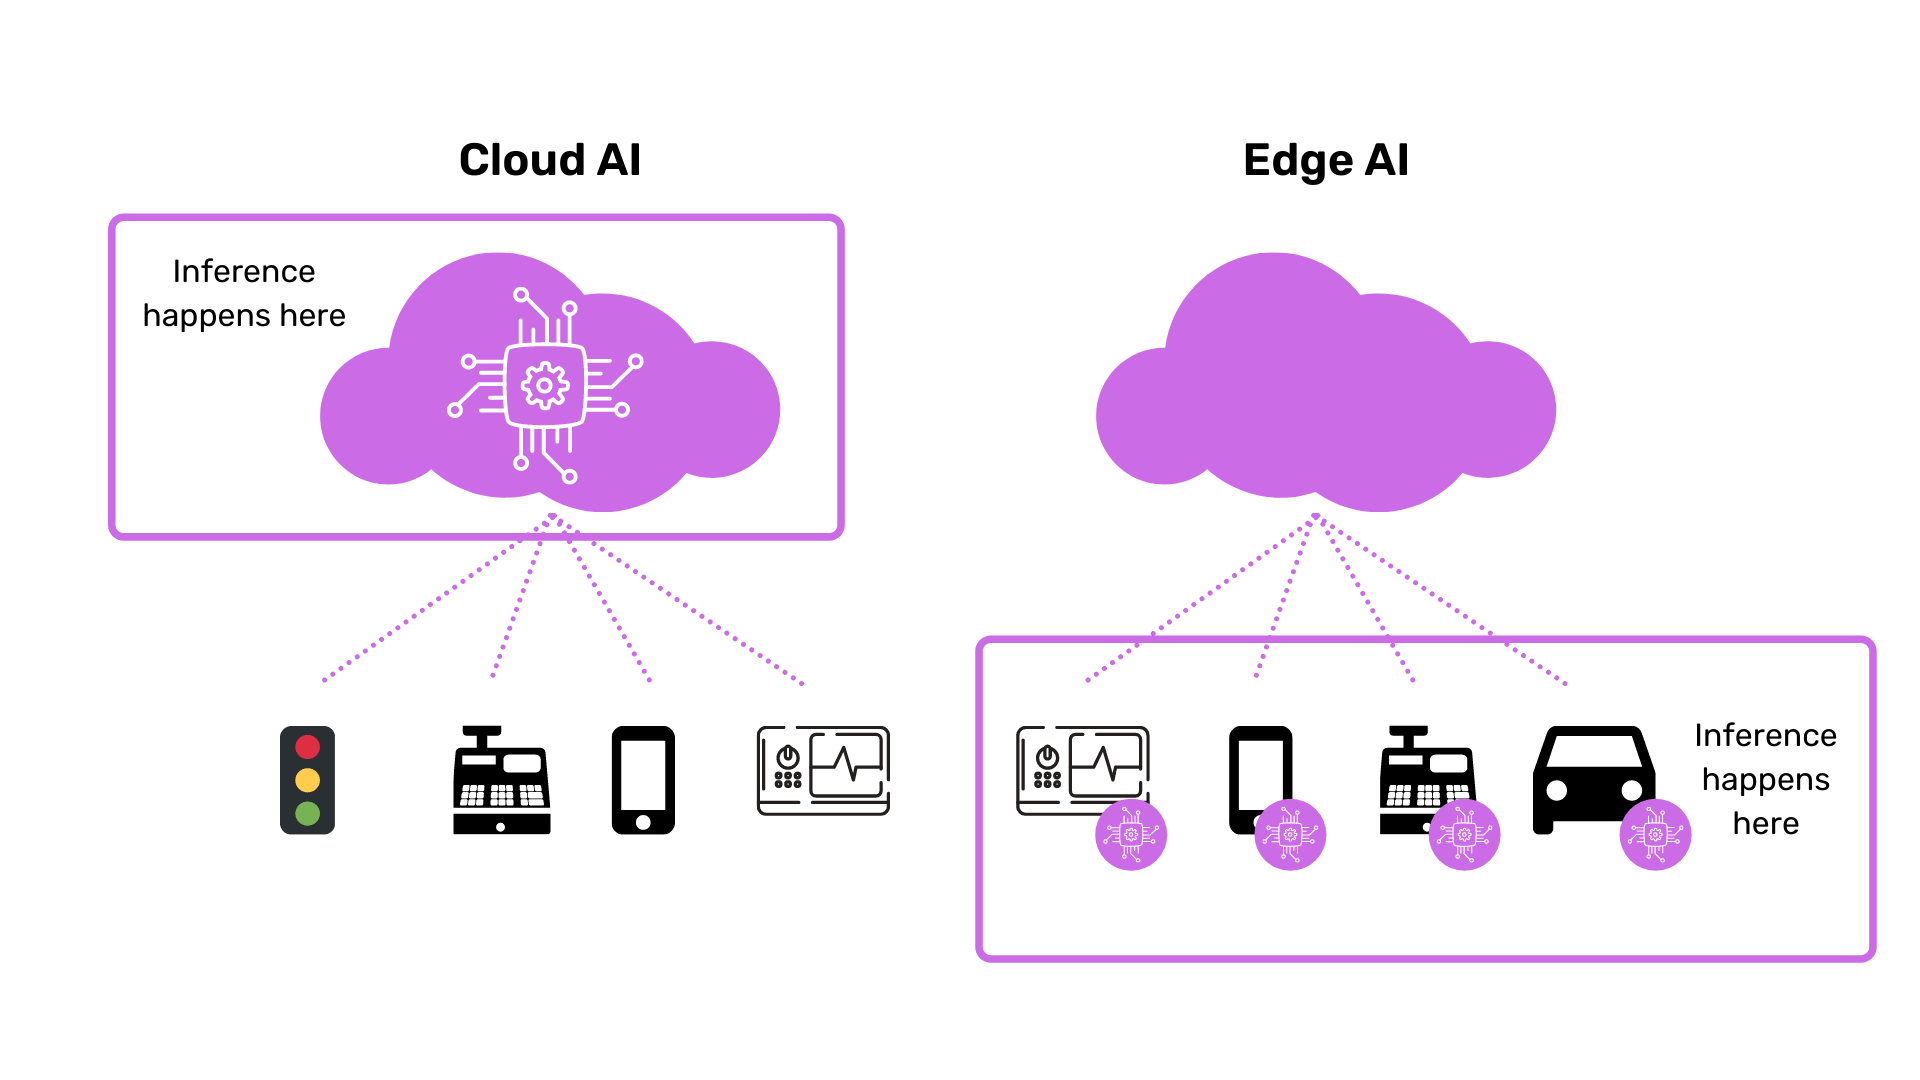
\includegraphics[width=0.6\textwidth]{image/CloudAIvsEdgeAI-1920w.png}
    \caption{Cloud AI và Edge AI}
    \label{fig:cloud_edge_ai}
\end{figure}

Trong đề tài này, Edge AI được triển khai như một module phân tích dữ liệu chuỗi thời gian (Time Series), đảm nhiệm chức năng dự báo sớm nồng độ bụi mịn PM2.5 dựa trên các thông số môi trường thực tế ngay tại hiện trường.

\subsection{Tổng quan mô hình TCN (Temporal Convolutional Network) và lý do lựa chọn TCN}

\subsubsection{Tổng quan về kiến trúc TCN}

Temporal Convolutional Network (TCN) là một kiến trúc mạng nơ-ron được thiết kế chuyên biệt cho bài toán xử lý dữ liệu chuỗi thời gian. Mô hình này kết hợp ưu điểm của mạng tích chập (Convolutional Neural Network -- CNN) với khả năng học các phụ thuộc dài hạn tương tự như mạng hồi tiếp (Recurrent Neural Network -- RNN) \cite{li2023_tcn_bilstm_dmattention,wang2024_causal_stan}.

\begin{figure}[H]
    \centering
    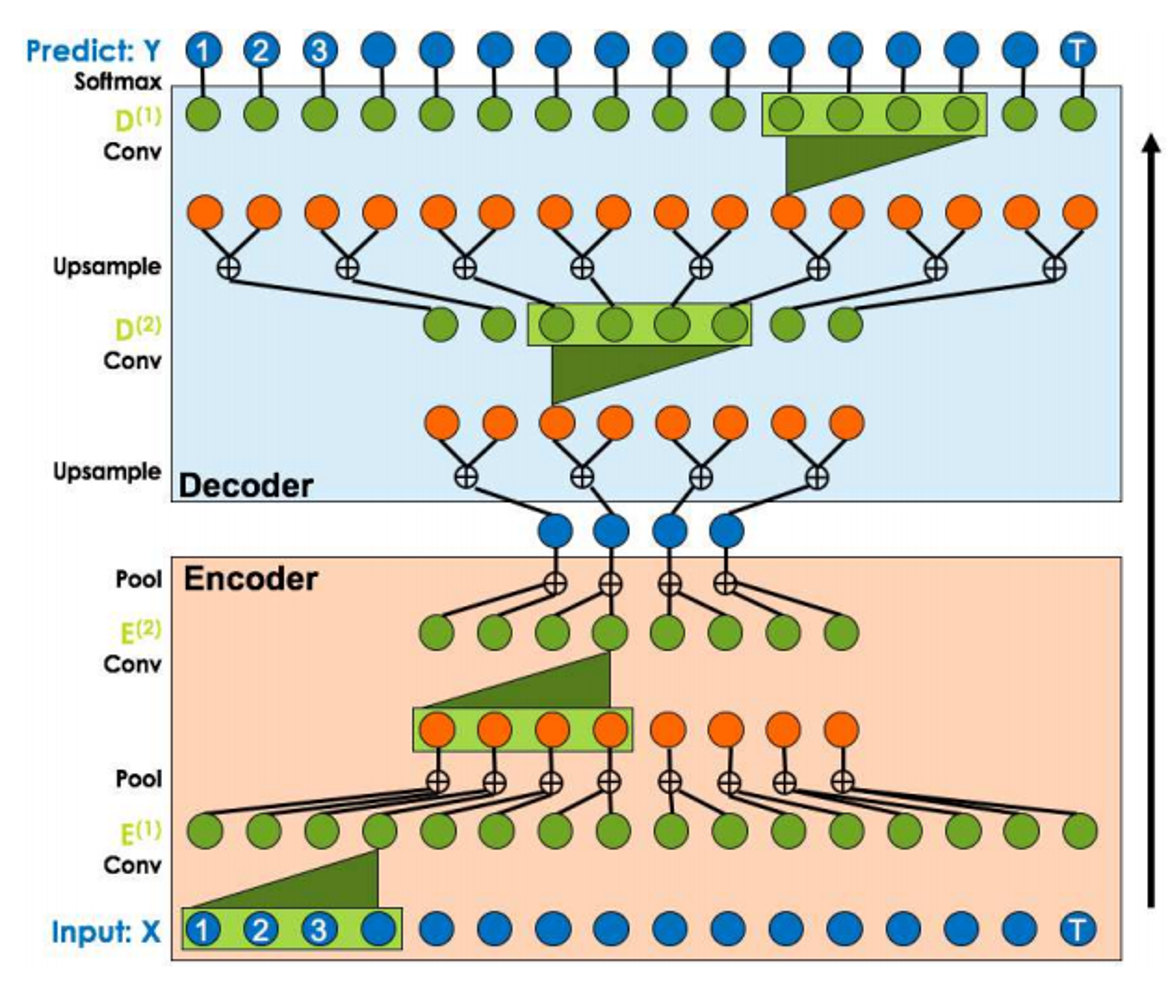
\includegraphics[width=0.5\textwidth]{image/TCN.png}
    \caption{Kiến trúc mô hình TCN}
    \label{fig:tcn_architecture}
\end{figure}

Kiến trúc TCN được xây dựng dựa trên hai nguyên lý cốt lõi:

\begin{itemize}
    \item \textbf{Causal Convolution (Tích chập nhân quả):}
    Đảm bảo rằng tại thời điểm $t$, mô hình chỉ sử dụng các thông tin từ các thời điểm trước đó và hiện tại, tức là từ $0$ đến $t$. Điều này giúp ngăn chặn hiện tượng ``rò rỉ'' thông tin từ tương lai vào quá trình dự báo.

    \item \textbf{Dilated Convolution (Tích chập giãn cách):}
    Các phần tử trong bộ lọc được áp dụng với khoảng cách giãn $d$, giúp mở rộng trường thụ cảm (\textit{receptive field}) theo cấp số nhân mà không làm tăng đáng kể số lượng tham số của mô hình.
\end{itemize}

Trong đề tài này, mô hình được cấu hình với các hệ số giãn cách:
\[
d = \{1, 2, 4, 8\}
\]

Cấu hình này cho phép mô hình quan sát hiệu quả các biến động của nồng độ bụi mịn PM2.5 trong khoảng thời gian 30 phút trước đó, từ đó nâng cao khả năng dự báo cho các bước thời gian tiếp theo.

\subsubsection{Lý do lựa chọn TCN thay vì LSTM/RNN}

Sau quá trình thực nghiệm và tối ưu hóa cho hệ thống Edge AI, trong luận văn nhóm đã lựa chọn kiến trúc TCN thay thế cho các mô hình LSTM và RNN nhờ nhiều ưu điểm về hiệu năng và khả năng triển khai trên thiết bị nhúng. Khác với RNN và LSTM phải xử lý dữ liệu tuần tự theo từng bước thời gian, TCN sử dụng phép tích chập trên toàn bộ chuỗi dữ liệu, cho phép tận dụng khả năng tính toán song song của phần cứng nhằm giảm đáng kể thời gian huấn luyện và suy luận. Ngoài ra, cấu trúc tích chập phân tầng kết hợp với residual connection giúp TCN giảm hiện tượng mất mát đạo hàm và học ổn định hơn khi xử lý các phụ thuộc dài hạn trong chuỗi thời gian.

Bên cạnh đó, TCN cho phép điều chỉnh linh hoạt trường thụ cảm thông qua các tham số như \texttt{kernel\_size} và \texttt{dilations}, giúp kiểm soát hiệu quả độ dài chuỗi dữ liệu được sử dụng để dự báo. Nhiều nghiên cứu gần đây cũng cho thấy TCN đạt hiệu quả cao trong các bài toán dự báo chất lượng không khí và nồng độ PM2.5 \cite{li2023_tcn_bilstm_dmattention,wang2024_causal_stan,stoten2025_pm25}. Ngoài hiệu quả dự báo, kiến trúc TCN còn có cấu trúc gọn nhẹ, số lượng tham số thấp và dễ dàng chuyển đổi sang định dạng TensorFlow Lite Float16. Trong đề tài này, mô hình sau khi lượng tử hóa đã giảm khoảng 50\% dung lượng lưu trữ nhưng vẫn duy trì độ chính xác dự báo ở mức cao, phù hợp để triển khai trên các thiết bị Edge AI như Raspberry Pi 4.

\subsection{Định dạng mô hình trung gian và tối ưu hóa trên thiết bị Edge}

\subsubsection{Định dạng mô hình ONNX (Open Neural Network Exchange)}

ONNX (Open Neural Network Exchange) là một định dạng mở được thiết kế để biểu diễn các mô hình học máy, cho phép chuyển đổi linh hoạt giữa nhiều framework khác nhau như PyTorch, TensorFlow và Keras.

\begin{figure}[H]
    \centering
    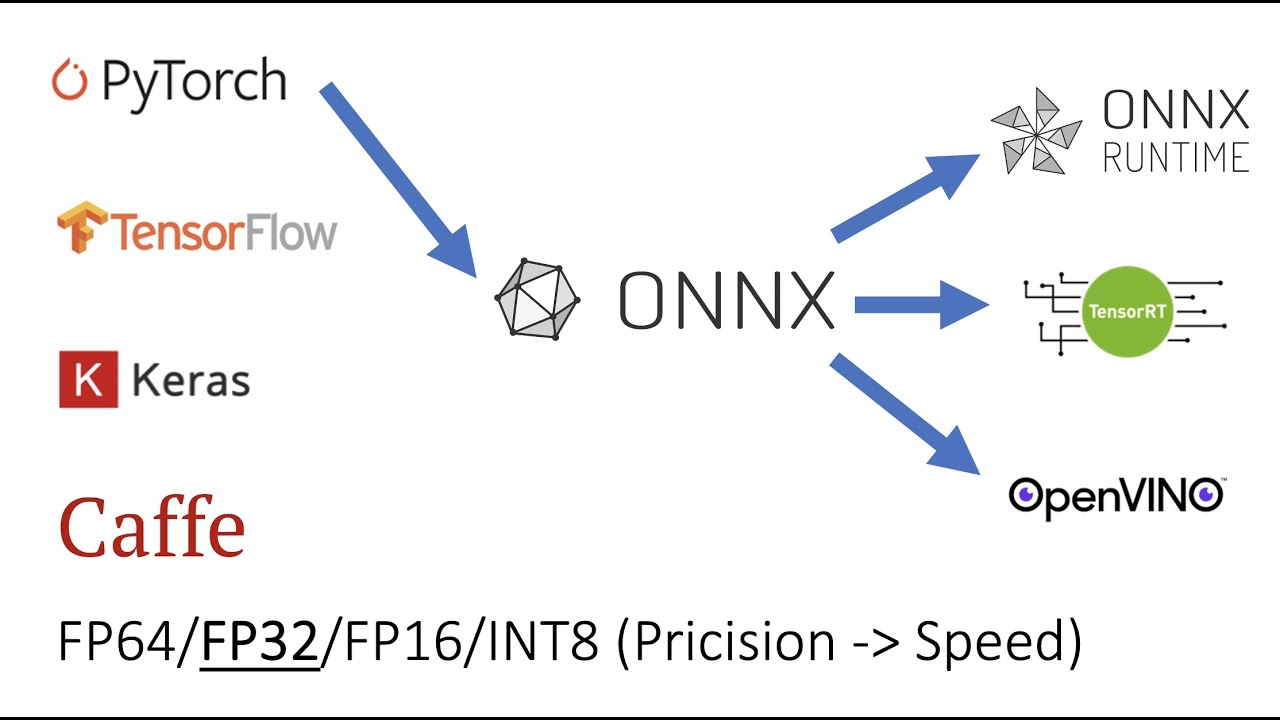
\includegraphics[width=0.6\textwidth]{image/ONNX.jpg}
    \caption{Định dạng ONNX}
    \label{fig:onnx}
\end{figure}

Trong đề tài này, ONNX đóng vai trò như một ``ngôn ngữ chung'' cho mô hình học sâu. Việc chuyển đổi mô hình sang định dạng ONNX giúp hệ thống có thể tận dụng các công cụ tối ưu hóa và các bộ tăng tốc phần cứng khác nhau mà không phụ thuộc vào môi trường huấn luyện ban đầu.

Một ưu điểm quan trọng của ONNX là khả năng tối ưu hóa đồ thị tính toán (\textit{graph optimization}), bao gồm việc loại bỏ các nút dư thừa, hợp nhất các phép toán liên tiếp và đơn giản hóa cấu trúc mô hình nhằm cải thiện tốc độ suy luận.

\subsubsection{Định dạng TensorFlow Lite (TFLite) và tối ưu hóa Float16}

TensorFlow Lite (TFLite) là thư viện mã nguồn mở được phát triển nhằm tối ưu hóa quá trình suy luận (\textit{inference}) trên các thiết bị di động và hệ thống nhúng có tài nguyên phần cứng hạn chế.

\begin{figure}[H]
    \centering
    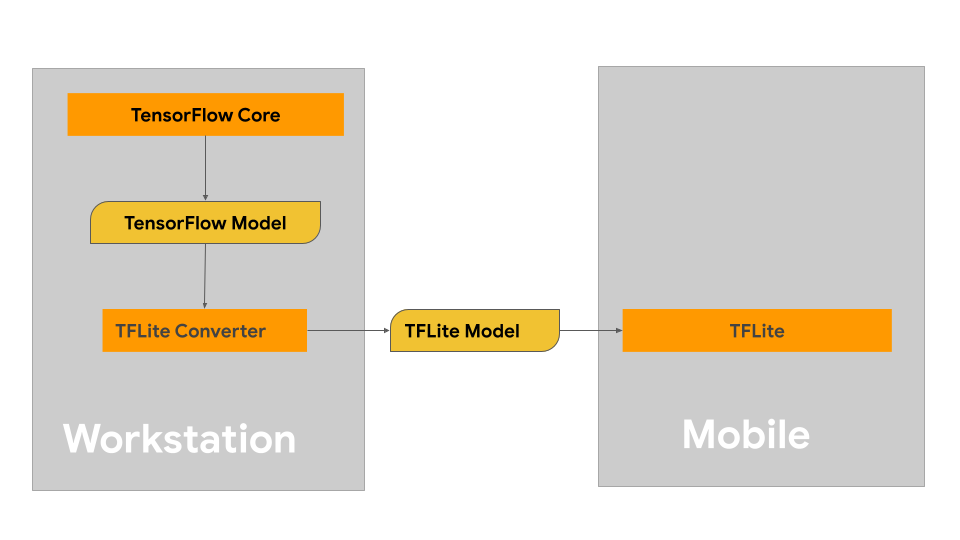
\includegraphics[width=0.6\textwidth]{image/TFLITE.png}
    \caption{Định dạng TensorFlow Lite}
    \label{fig:tflite}
\end{figure}

Trong hệ thống được xây dựng, kỹ thuật \textit{Float16 Quantization} được áp dụng trong quá trình chuyển đổi mô hình (thực hiện trong file \texttt{convert.py}). Cụ thể, các trọng số của mô hình được chuyển từ định dạng số thực dấu phẩy động 32-bit (Float32) sang 16-bit (Float16).

Việc lượng tử hóa Float16 mang lại các lợi ích sau:

\begin{itemize}
    \item \textbf{Giảm dung lượng mô hình:}
    Kích thước tệp mô hình giảm khoảng 50\% so với mô hình gốc, giúp tiết kiệm bộ nhớ lưu trữ trên thiết bị nhúng.

    \item \textbf{Tăng tốc độ suy luận:}
    Nhiều bộ xử lý hiện đại hỗ trợ tính toán Float16 hiệu quả, giúp giảm độ trễ (\textit{latency}) khi dự báo chỉ số PM2.5 theo thời gian thực.

    \item \textbf{Duy trì độ chính xác cao:}
    So với lượng tử hóa Int8, định dạng Float16 thường giữ được độ chính xác gần như tương đương với mô hình gốc, đồng thời ít gây sai lệch kết quả dự báo.
\end{itemize}

\section{Giao tiếp phần cứng công nghiệp}
\subsection{Chuẩn vật lý RS485}
\begin{figure}[H]
    \centering
    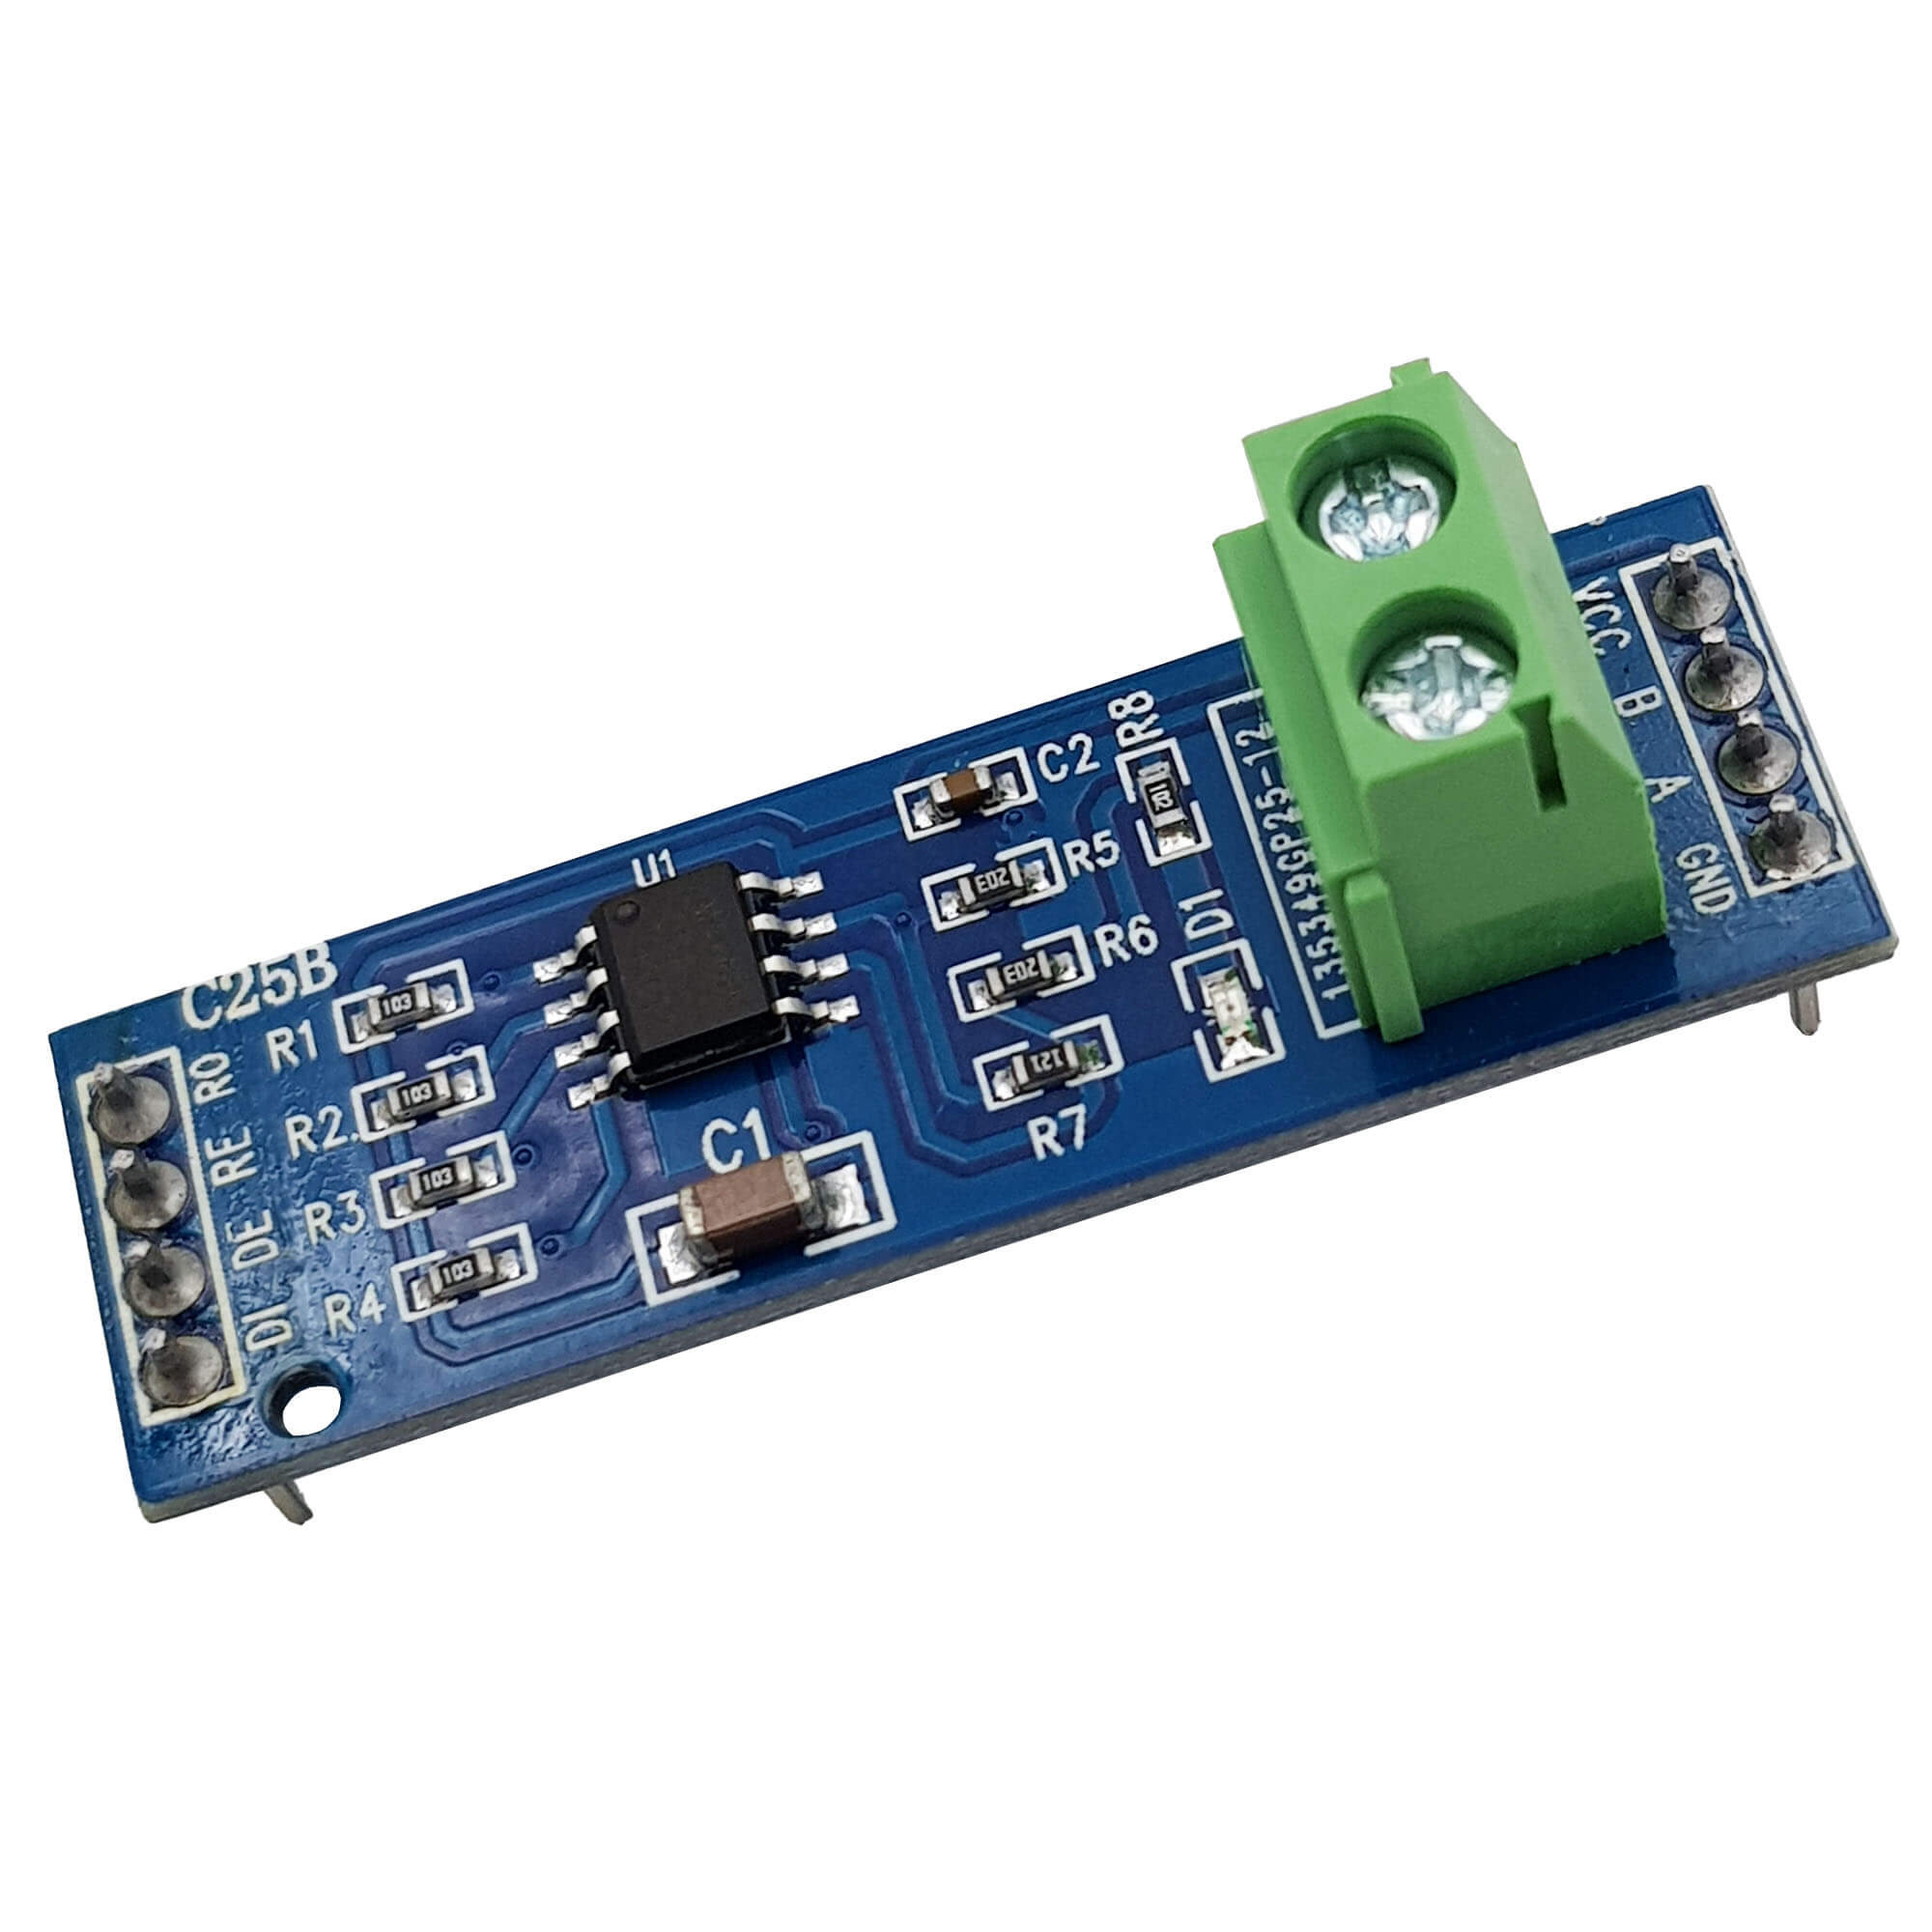
\includegraphics[width=0.2\linewidth]{image/rs485.jpg}
    \caption{RS485 TTL }
    \label{fig:placeholder}
\end{figure}
Chuẩn RS485 (Recommended Standard 485) là một chuẩn truyền thông ở tầng vật lý, được Hiệp hội Công nghiệp Điện tử (EIA) ban hành nhằm phục vụ các hệ thống truyền dữ liệu nối tiếp trong môi trường công nghiệp. RS485 được thiết kế để đáp ứng yêu cầu truyền dữ liệu ổn định trên khoảng cách xa, chống nhiễu tốt và hỗ trợ nhiều thiết bị cùng kết nối trên một đường truyền, do đó được sử dụng rộng rãi trong các hệ thống điều khiển, giám sát và tự động hóa công nghiệp.


Về mặt nguyên lý hoạt động, RS485 sử dụng phương pháp truyền tín hiệu vi sai (differential signaling) thông qua hai dây tín hiệu A và tín hiệu B. Dữ liệu được biểu diễn bằng sự chênh lệch điện áp giữa hai dây này thay vì so với mass (hoặc GND) như các chuẩn truyền đơn cực. Cách truyền vi sai giúp RS485 có khả năng chống nhiễu điện từ cao, đặc biệt phù hợp với môi trường công nghiệp nơi tồn tại nhiều nguồn nhiễu như động cơ, biến tần và thiết bị công suất lớn.

Nhờ các đặc tính nổi bật như khả năng truyền xa, chống nhiễu tốt, hỗ trợ nhiều thiết bị và chi phí triển khai thấp, chuẩn RS485 vẫn giữ vai trò quan trọng trong các hệ thống công nghiệp hiện đại. Mặc dù đã xuất hiện nhiều chuẩn truyền thông mới, RS485 vẫn là lựa chọn ưu tiên trong các ứng dụng yêu cầu độ tin cậy cao, cấu trúc đơn giản và khả năng hoạt động ổn định trong môi trường khắc nghiệt.

Trong hệ thống IoT và Linux Embedded, RS485 thường được kết hợp với các giao thức truyền thông công nghiệp như Modbus RTU nhằm hỗ trợ trao đổi dữ liệu giữa gateway và các cảm biến hoặc thiết bị điều khiển.
\subsection{Giao thức Modbus RTU và cấu trúc khung tin}
\subsubsection{Giao thức Modbus RTU}


Modbus RTU (Remote Terminal Unit) là một giao thức truyền thông công nghiệp phổ biến, được phát triển bởi Modicon vào năm 1979. Đây là giao thức dạng master–slave (hiện nay còn gọi là client–server), được thiết kế nhằm cho phép các thiết bị điều khiển và giám sát trong công nghiệp trao đổi dữ liệu với nhau một cách đơn giản, tin cậy và hiệu quả. Nhờ tính mở, dễ triển khai và khả năng tương thích cao, Modbus RTU hiện vẫn được sử dụng rộng rãi trong các hệ thống SCADA, PLC, cảm biến và thiết bị đo lường công nghiệp.

Trong mô hình hoạt động của Modbus RTU, thiết bị master đóng vai trò khởi tạo và điều khiển toàn bộ quá trình truyền thông, trong khi các thiết bị slave chỉ phản hồi khi nhận được yêu cầu hợp lệ từ master. Mỗi thiết bị slave được gán một địa chỉ duy nhất trên bus, giúp master xác định đúng thiết bị cần giao tiếp. Cơ chế này giúp tránh xung đột dữ liệu và đảm bảo tính tuần tự trong quá trình truyền thông.


\subsubsection{Cấu trúc khung tin}


Modbus RTU truyền dữ liệu dưới dạng các khung tin (frame) được mã hóa theo dạng nhị phân, cho phép tiết kiệm băng thông và nâng cao hiệu quả truyền thông. Mỗi khung tin Modbus RTU bao gồm các trường dữ liệu được sắp xếp theo thứ tự xác định, đảm bảo thiết bị nhận có thể giải mã chính xác nội dung thông tin.


Một khung tin Modbus RTU tiêu chuẩn bao gồm các thành phần chính: địa chỉ thiết bị, mã hàm, vùng dữ liệu và mã kiểm tra lỗi CRC. Khung tin được phân tách với các khung khác bằng một khoảng im lặng trên đường truyền (silent interval), có độ dài tối thiểu tương đương 3.5 ký tự, giúp thiết bị nhận xác định ranh giới giữa các khung dữ liệu.


Trường địa chỉ thiết bị có độ dài 1 byte, dùng để xác định slave mà master muốn giao tiếp. Địa chỉ hợp lệ nằm trong khoảng từ 1 đến 247, trong khi địa chỉ 0 được sử dụng cho chế độ broadcast, cho phép master gửi lệnh đến tất cả các slave mà không yêu cầu phản hồi.


Mỗi khung tin Modbus RTU kết thúc bằng trường CRC (Cyclic Redundancy Check) dài 2 byte. CRC được sử dụng để kiểm tra lỗi trong quá trình truyền dữ liệu, giúp phát hiện các lỗi do nhiễu hoặc sai lệch tín hiệu trên đường truyền. Slave hoặc master sẽ tự động tính toán CRC của khung tin nhận được và so sánh với giá trị CRC đi kèm để xác định tính toàn vẹn của dữ liệu.


Mặc dù đã xuất hiện nhiều giao thức truyền thông công nghiệp hiện đại hơn, Modbus RTU vẫn giữ vai trò quan trọng trong thực tế nhờ độ ổn định, tính phổ biến và khả năng tương thích rộng rãi. Việc hiểu rõ nguyên lý hoạt động và cấu trúc khung tin Modbus RTU là nền tảng quan trọng cho việc thiết kế, triển khai và vận hành các hệ thống giám sát và điều khiển công nghiệp.

\section{Kết nối Cloud và IoT}
\subsection{Tổng quan về CoreIOT}

\begin{figure}[H]
    \centering
    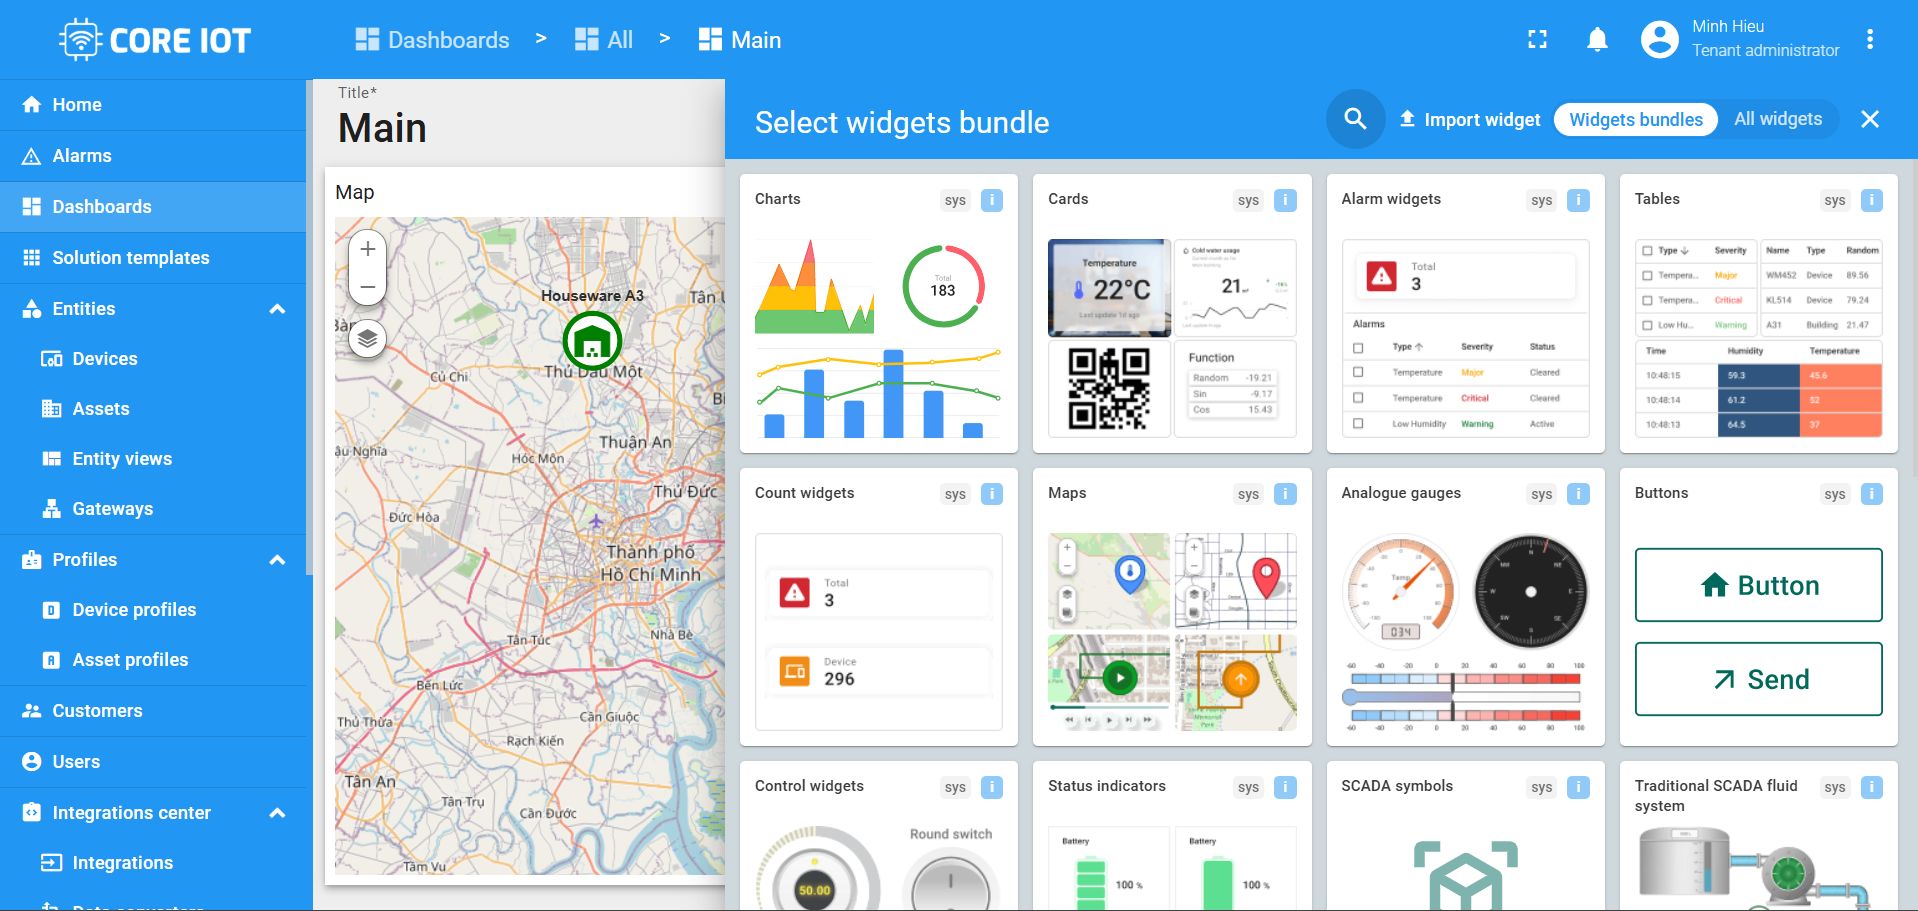
\includegraphics[width=1\textwidth]{image/coreiotp.png}
    \caption{Tổng quan về CoreIOT}
    \label{fig:coreiot}
\end{figure}

CoreIoT là một nền tảng Internet of Things (IoT) được phát triển và xây
dựng dựa trên định hướng tương tự các nền tảng IoT mã nguồn mở phổ biến như
ThingsBoard, nhằm phục vụ nhu cầu giảng dạy, nghiên cứu và triển khai các bài
toán IoT trong môi trường học thuật và đào tạo kỹ thuật. Nền tảng được tùy
biến và phát triển lại để phù hợp với điều kiện sử dụng, ngôn ngữ và đối tượng
người dùng là sinh viên, giảng viên và các nhóm nghiên cứu tại nhà trường.

Về mặt kiến trúc tổng thể, CoreIoT được thiết kế theo mô hình nền tảng trung
tâm, cho phép thu thập, xử lý, lưu trữ và hiển thị dữ liệu từ các thiết bị IoT
phân tán. Hệ thống đóng vai trò trung gian giữa các thiết bị đầu cuối và người
dùng, hỗ trợ quản lý thiết bị, giám sát dữ liệu theo thời gian thực và xây dựng
các ứng dụng IoT hoàn chỉnh. Cách tiếp cận này giúp người học dễ dàng tiếp cận
các khái niệm cốt lõi của IoT mà không cần triển khai toàn bộ hạ tầng từ đầu.

CoreIoT hỗ trợ kết nối với các thiết bị IoT thông qua các giao thức truyền
thông phổ biến, đặc biệt phù hợp với các thiết bị nhúng và hệ thống công nghiệp.
Dữ liệu từ cảm biến sau khi được thu thập tại thiết bị biên sẽ được truyền về
nền tảng để xử lý và lưu trữ tập trung. Thông qua đó, CoreIoT cho phép theo
dõi trạng thái thiết bị, phân tích dữ liệu và hiển thị thông tin trực quan trên
dashboard, hỗ trợ người dùng giám sát hệ thống một cách hiệu quả.

Bên cạnh chức năng giám sát, CoreIoT còn hỗ trợ xây dựng các quy tắc xử lý
dữ liệu và sự kiện thông qua cơ chế xử lý logic ở tầng nền tảng. Các quy tắc này
cho phép hệ thống phản ứng tự động trước các điều kiện cụ thể, chẳng hạn như
phát cảnh báo khi giá trị cảm biến vượt ngưỡng hoặc ghi nhận sự kiện phục vụ
phân tích sau này. Cách tiếp cận này giúp người học hiểu rõ hơn về mô hình xử
lý dữ liệu và tự động hóa trong các hệ thống IoT hiện đại.

Với định hướng phục vụ đào tạo và nghiên cứu, CoreIoT không chỉ đóng vai
trò là một công cụ giám sát mà còn là môi trường thực hành giúp sinh viên tiếp
cận các khái niệm quan trọng như quản lý thiết bị, truyền thông IoT, xử lý dữliệu thời gian thực và tích hợp hệ thống. Nền tảng tạo điều kiện thuận lợi cho
việc triển khai các đề tài học tập, đồ án và nghiên cứu ứng dụng, đồng thời có
khả năng mở rộng để đáp ứng các bài toán IoT phức tạp hơn trong tương lai.


\subsection{Giao thức MQTT trong hệ thống nhúng}
\begin{figure}[!h]
    \centering
    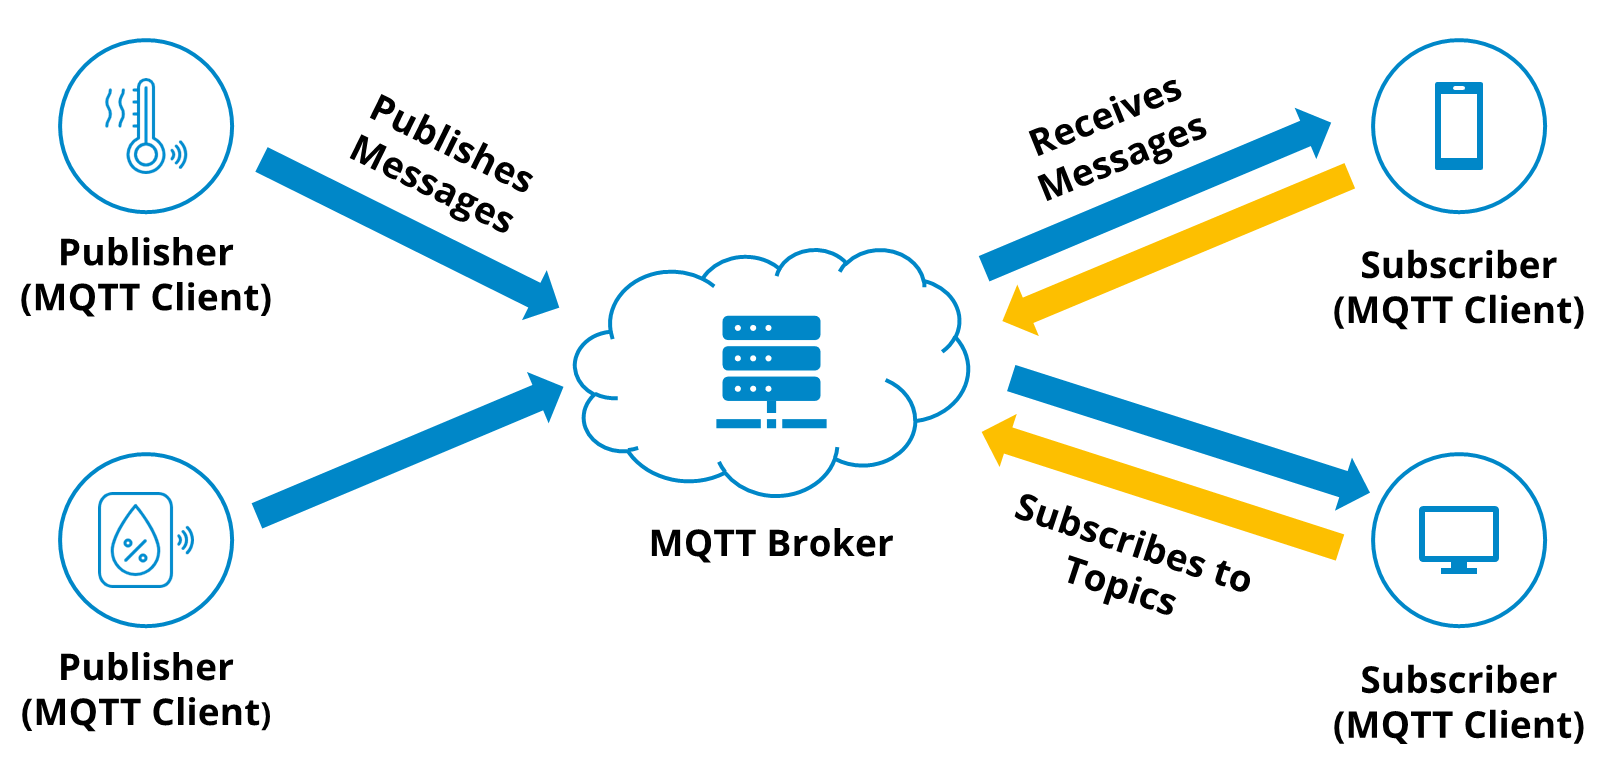
\includegraphics[width=0.6\textwidth]{image/mqtt1.png}
    \caption{Giao thức MQTT trong hệ thống nhúng}
    \label{fig:mqtt}

\end{figure}

MQTT (Message Queuing Telemetry Transport) là một giao thức truyền tin
nhẹ, được thiết kế theo mô hình publish–subscribe, đặc biệt phù hợp cho các
hệ thống IoT có tài nguyên hạn chế và yêu cầu truyền dữ liệu với độ trễ thấp.
Trong mô hình này, các thiết bị không giao tiếp trực tiếp với nhau mà thông
qua một thành phần trung gian gọi là broker. Thiết bị gửi dữ liệu sẽ đóng vai
trò publisher, trong khi thiết bị nhận dữ liệu là subscriber, và broker chịu trách
nhiệm phân phối thông điệp dựa trên các chủ đề (topic).

Một đặc điểm nổi bật của MQTT là kích thước gói tin nhỏ, giúp giảm băng thông và tiết kiệm năng lượng, rất phù hợp với các thiết bị nhúng và mạng truyền
thông không ổn định. MQTT hỗ trợ nhiều mức chất lượng dịch vụ (Quality of
Service – QoS), cho phép cân bằng giữa độ tin cậy và hiệu năng truyền thông.
Bên cạnh đó, giao thức còn hỗ trợ cơ chế giữ kết nối (keep-alive), thông báo trạng
thái thiết bị và khả năng mở rộng linh hoạt trong các hệ thống IoT quy mô lớn.
Nhờ các đặc tính trên, MQTT thường được sử dụng trong các ứng dụng giám
sát thời gian thực, thu thập dữ liệu cảm biến, hệ thống điều khiển từ xa và các
nền tảng IoT trung tâm như CoreIoT hoặc các nền tảng tương đương.



\chapter{Thiết kế hệ thống}
\textcolor{chaptercolor}{\textit{Chương này tập trung vào việc phân tích bài toán quản lý cảnh báo trong nhà kho, xác định các yêu cầu của hệ thống và xây dựng thiết kế các chức năng cho hệ thống giám sát.
}}

\begin{enumerate}[
    leftmargin=2.5em,
    labelsep=0.8em,
    itemsep=0.6em
]
  \renewcommand{\labelenumi}{\textcolor{chaptercolor}{\bfseries \thechapter.\arabic{enumi}}}

  \item \textbf{Phân tích yêu cầu}
  \item \textbf{Thiết kế nền tảng}
  \item \textbf{Thiết kế khối xử lý}
  \item \textbf{Thiết kế giao diện người dùng}
\end{enumerate}
\newpage
\section{Phân tích yêu cầu}
\section{Thiết kế nền tảng}
\subsection{Thiết kế cơ chế truyền dữ liệu giữa Gateway và CoreIoT}

Trong hệ thống được xây dựng, Raspberry Pi 4 đóng vai trò gateway trung tâm, thực hiện chức năng thu thập dữ liệu từ các cảm biến, xử lý trạng thái hệ thống và truyền dữ liệu lên nền tảng quản lý IoT CoreIoT. Để đáp ứng yêu cầu truyền dữ liệu theo thời gian thực với mức tiêu thụ tài nguyên thấp, hệ thống sử dụng giao thức MQTT làm cơ chế giao tiếp chính giữa gateway và cloud server.

Gateway thực hiện kết nối đến MQTT Broker tại địa chỉ \texttt{App.\allowbreak coreiot.\allowbreak io} thông qua cổng \texttt{1883}. Quá trình xác thực sử dụng access token của thiết bị làm username cho phiên kết nối MQTT. Sau khi kết nối thành công, thiết bị định kỳ publish dữ liệu lên topic \texttt{v1/\allowbreak devices/\allowbreak me/\allowbreak telemetry} với chu kỳ 5 giây nhằm phục vụ việc giám sát và lưu trữ dữ liệu trên nền tảng cloud.

Dữ liệu được truyền lên hệ thống được đóng gói dưới dạng JSON nhằm đảm bảo tính linh hoạt và khả năng mở rộng trong quá trình xử lý phía server. Payload bao gồm các thông số môi trường được thu thập từ hệ thống cảm biến như nhiệt độ, độ ẩm, áp suất, cường độ ánh sáng và nồng độ bụi mịn PM2.5. Các giá trị này lần lượt được đọc từ các file trong hệ thống file của Linux như:

\begin{itemize}
    \item \texttt{/sys/class/sensorhub/hub0/temp}: dữ liệu nhiệt độ.
    \item \texttt{/sys/class/sensorhub/hub0/hum}: dữ liệu độ ẩm.
    \item \texttt{/sys/class/sensorhub/hub0/pressure}: dữ liệu áp suất môi trường.
    \item \texttt{/sys/class/sensorhub/hub0/lux}: dữ liệu cường độ ánh sáng.
    \item \texttt{/sys/class/sensorhub/hub0/pm25}: dữ liệu bụi mịn PM2.5.
\end{itemize}

Ngoài dữ liệu cảm biến thời gian thực, hệ thống còn tích hợp giá trị dự báo nồng độ PM2.5 trong 15 phút tiếp theo thông qua file tạm \texttt{/tmp/ai\_predict.txt}. Giá trị này được sử dụng nhằm hỗ trợ cơ chế cảnh báo sớm và nâng cao khả năng giám sát môi trường trong hệ thống kho thông minh.

Bên cạnh các thông số cảm biến, payload còn chứa các trường dữ liệu bổ trợ như mã thiết bị (\texttt{node}), chế độ hoạt động của hệ thống (\texttt{mode}) và timestamp thời gian thực được sinh từ hệ điều hành Linux thông qua hàm \texttt{time.time()}. Việc bổ sung timestamp giúp đảm bảo khả năng đồng bộ dữ liệu và hỗ trợ quá trình lưu trữ, truy vết dữ liệu trên nền tảng quản lý.

Trước khi dữ liệu được gửi lên MQTT Broker, gateway thực hiện một số bước tiền xử lý nhằm chuẩn hóa dữ liệu và xác định trạng thái hoạt động của hệ thống. Các giá trị cảm biến được đọc dưới dạng dữ liệu thô và được quy đổi sang giá trị thực tế thông qua các hệ số chia tương ứng. Trong đó, dữ liệu nhiệt độ được chia cho 10 để chuyển đổi sang đơn vị độ C, dữ liệu áp suất được chia cho 100 để đưa về đơn vị tiêu chuẩn, trong khi các thông số còn lại được giữ nguyên hoặc xử lý tùy theo đặc tính của từng cảm biến.

Sau giai đoạn tiền xử lý dữ liệu, gateway tiến hành đánh giá trạng thái vận hành của hệ thống dựa trên các ngưỡng cảnh báo đã được thiết lập trước. Quá trình đánh giá này nhằm xác định mức độ an toàn của môi trường kho và đưa ra cơ chế điều khiển phù hợp đối với quạt làm mát và relay.

Trong trường hợp nhiệt độ vượt quá 45\textdegree C hoặc giá trị dự báo PM2.5 lớn hơn 100, hệ thống sẽ lập tức chuyển sang trạng thái khẩn cấp \texttt{EMERGENCY\_FIRE}. Khi đó, quạt làm mát được kích hoạt ở mức cao nhất nhằm giảm thiểu nguy cơ mất an toàn trong môi trường vận hành.

Đối với điều kiện hoạt động thông thường, trạng thái hệ thống và mức điều khiển quạt được xác định dựa trên ngưỡng nhiệt độ như trình bày trong Bảng \ref{tab:system_state_logic}.

\begin{table}[H]
\centering
\begin{tabular}{|c|c|c|}
\hline
\textbf{Điều kiện} & \textbf{Trạng thái hệ thống} & \textbf{Mức quạt} \\ \hline
Nhiệt độ $<$ 30\textdegree C & NORMAL & LOW \\ \hline
30\textdegree C $\leq$ Nhiệt độ $<$ 40\textdegree C & WARNING & MEDIUM \\ \hline
Nhiệt độ $\geq$ 40\textdegree C & CRITICAL & HIGH \\ \hline
Nhiệt độ $>$ 45\textdegree C hoặc PM2.5 dự báo $>$ 100 & EMERGENCY\_FIRE & HIGH \\ \hline
\end{tabular}
\caption{Cơ chế xác định trạng thái hệ thống}
\label{tab:system_state_logic}
\end{table}

Bên cạnh cơ chế điều khiển theo ngưỡng nhiệt độ, hệ thống còn triển khai cơ chế giám sát trạng thái kéo dài nhằm phát hiện các tình huống bất thường trong quá trình vận hành. Nếu quạt duy trì ở mức \texttt{HIGH} liên tục trong hơn 30 giây, gateway sẽ chuyển hệ thống sang trạng thái \texttt{EMERGENCY\_SYSTEM}. Cơ chế này giúp nâng cao khả năng giám sát và tăng mức độ an toàn cho hệ thống trong môi trường thực tế.

Song song với quá trình điều khiển quạt, relay cũng được điều khiển tự động dựa trên nhiệt độ môi trường. Relay sẽ được kích hoạt khi nhiệt độ vượt quá 25\textdegree C và tự động tắt khi nhiệt độ giảm xuống dưới ngưỡng quy định.

Sau khi hoàn tất quá trình xử lý và đánh giá trạng thái, gateway tiến hành tổng hợp toàn bộ dữ liệu cảm biến và trạng thái hệ thống thành một payload hoàn chỉnh trước khi gửi lên nền tảng CoreIoT thông qua giao thức MQTT. Payload được xây dựng dưới dạng JSON nhằm đảm bảo khả năng mở rộng và dễ dàng tích hợp với hệ thống backend.

Cấu trúc dữ liệu được gửi lên hệ thống được mô tả trong Bảng \ref{tab:api_payload}.

\begin{table}[H]
\centering
\begin{tabular}{|c|l|l|}
\hline
\textbf{Trường dữ liệu} & \textbf{Ý nghĩa} & \textbf{Ví dụ} \\ \hline
\texttt{temperature} & Nhiệt độ môi trường & 32.5 \\ \hline
\texttt{humidity} & Độ ẩm môi trường & 75 \\ \hline
\texttt{light\_intensity} & Cường độ ánh sáng & 420 \\ \hline
\texttt{pm25} & Nồng độ bụi mịn PM2.5 & 18 \\ \hline
\texttt{stat} & Trạng thái hệ thống & WARNING \\ \hline
\texttt{node} & Mã thiết bị gateway & ESP\_01 \\ \hline
\texttt{mode} & Chế độ hoạt động & day \\ \hline
\texttt{timestamp} & Thời gian gửi dữ liệu & 1715259000 \\ \hline
\end{tabular}
\caption{Cấu trúc payload dữ liệu gửi lên CoreIoT}
\label{tab:api_payload}
\end{table}

Từ cấu trúc trên, payload JSON được gửi lên MQTT Broker có dạng như sau:

\begin{verbatim}
{
    "temperature": 32.5,
    "humidity": 75,
    "light_intensity": 420,
    "pm25": 18,
    "stat": "WARNING",
    "node": "ESP_01",
    "mode": "day",
    "timestamp": "1715259000"
}
\end{verbatim}

Toàn bộ quá trình từ thu thập dữ liệu cảm biến, xử lý trạng thái hệ thống, xây dựng payload đến publish dữ liệu lên CoreIoT được thực hiện liên tục theo chu kỳ 5 giây thông qua vòng lặp chính của chương trình gateway. Để đảm bảo tính ổn định của hệ thống, các lỗi phát sinh trong quá trình đọc dữ liệu cảm biến hoặc truy xuất file dự báo AI đều được xử lý bằng cơ chế fallback, trong đó giá trị mặc định được gán bằng 0 nhằm tránh gián đoạn luồng dữ liệu gửi lên hệ thống cloud.
Quá trình thu thập dữ liệu, xử lý logic và truyền dữ liệu được thực hiện liên tục theo chu kỳ 5 giây thông qua vòng lặp chính của chương trình gateway. Để đảm bảo tính ổn định của hệ thống, các lỗi phát sinh trong quá trình đọc dữ liệu cảm biến hoặc truy xuất file dự báo AI đều được xử lý bằng cơ chế fallback, trong đó giá trị mặc định được gán bằng 0 nhằm tránh gián đoạn luồng dữ liệu gửi lên hệ thống cloud.

\begin{figure}[!h]
    \centering
    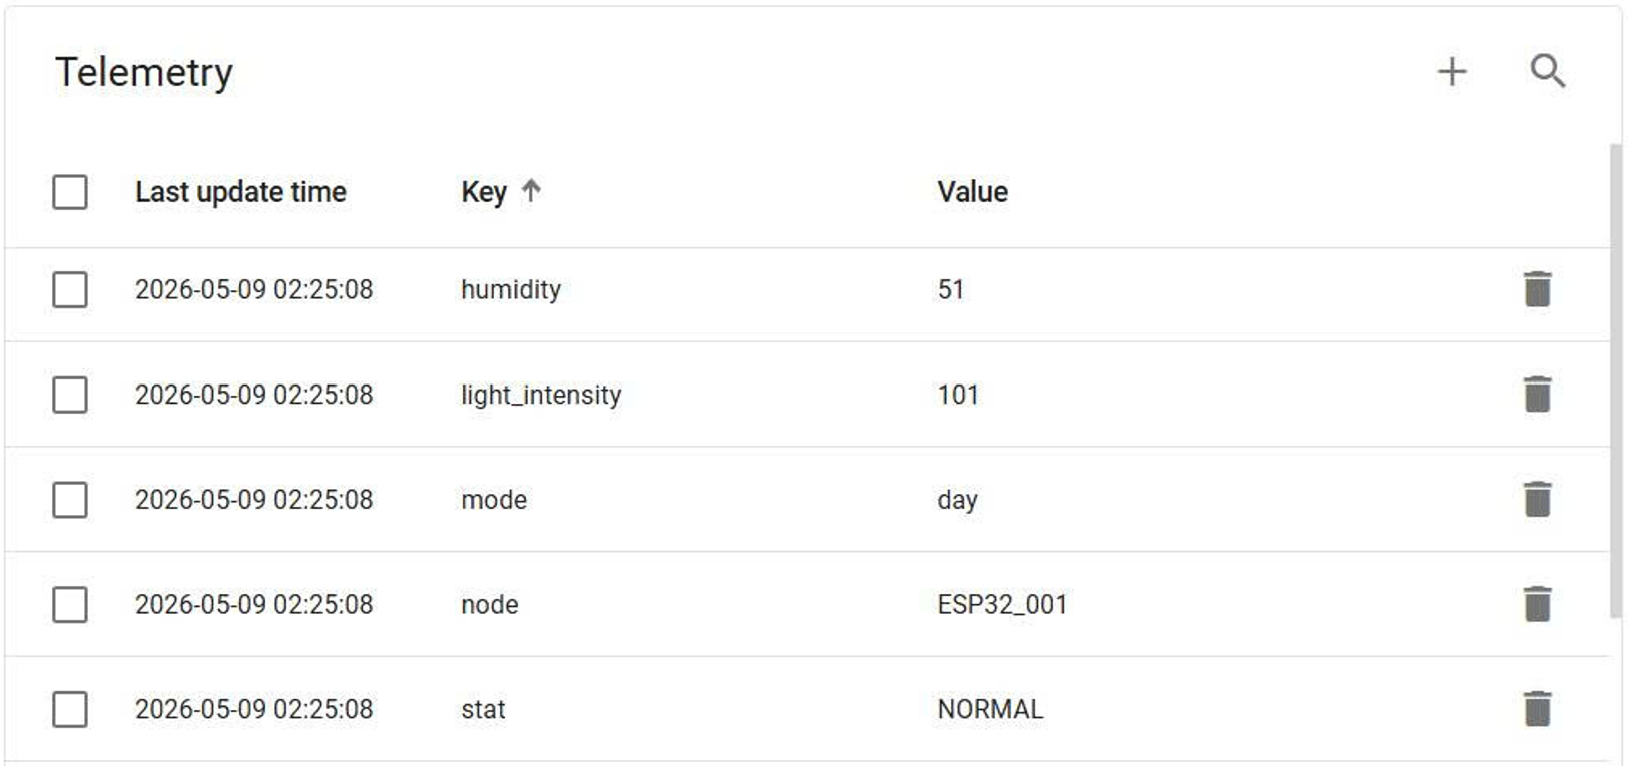
\includegraphics[width=1\textwidth]{image/api.png}
    \caption{Định dạng dữ liệu được gửi lên CoreIot}
    \label{fig:rulechain}
\end{figure}
\newpage

\section{Thiết kế khối xử lý}
\subsection{Khối xử lý cảnh báo}

Hình \ref{fig:warning_block} mô tả kiến trúc tổng thể của khối xử lý cảnh báo được triển khai trên nền tảng gateway sử dụng Raspberry Pi 4. Khối chức năng này có nhiệm vụ thu thập dữ liệu cảm biến, tiền xử lý dữ liệu, thực hiện phân tích bằng Rule Chain kết hợp AI, sau đó đưa ra mức cảnh báo phù hợp để hiển thị trên các giao diện giám sát.

\begin{figure}[H]
    \centering
    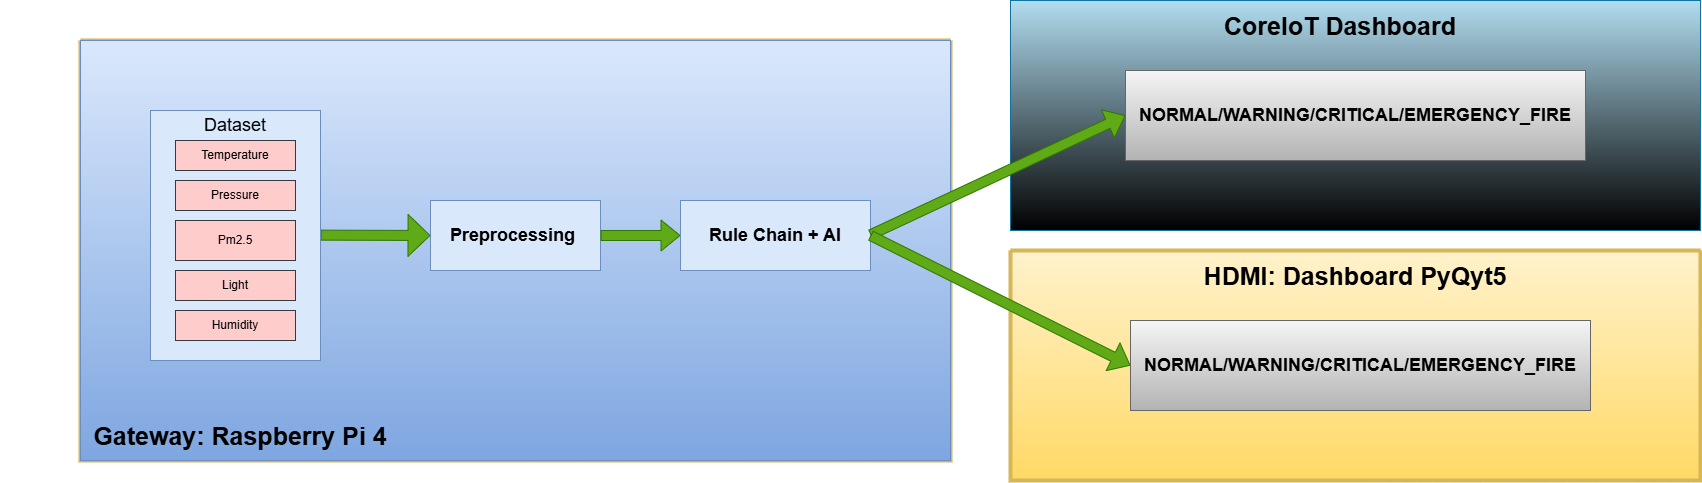
\includegraphics[width=0.95\linewidth]{image/warnblock.png}
    \caption{Kiến trúc khối xử lý cảnh báo trên gateway Raspberry Pi 4}
    \label{fig:warning_block}
\end{figure}

Trong hệ thống, các dữ liệu đầu vào bao gồm nhiệt độ (Temperature), áp suất (Pressure), bụi mịn PM2.5, cường độ ánh sáng (Light) và độ ẩm (Humidity). Các dữ liệu này được thu thập từ cảm biến thông qua các giao thức truyền thông như I2C và Modbus RTU RS485, sau đó được đưa vào gateway Raspberry Pi 4 để xử lý.

Sau khi tiếp nhận dữ liệu, hệ thống thực hiện bước \textbf{Preprocessing} nhằm chuẩn hóa dữ liệu đầu vào, loại bỏ nhiễu, kiểm tra giá trị bất thường và chuyển đổi dữ liệu về định dạng phù hợp cho quá trình phân tích. Đây là bước quan trọng giúp tăng độ ổn định và độ chính xác của hệ thống cảnh báo.

Tiếp theo, dữ liệu được đưa vào khối \textbf{Rule Chain + AI}. Tại đây, hệ thống áp dụng tập luật (Rule Chain) kết hợp với thuật toán AI nhằm đánh giá trạng thái môi trường theo thời gian thực. Các luật được xây dựng dựa trên ngưỡng an toàn của từng loại cảm biến, đồng thời AI hỗ trợ phân tích xu hướng và nhận diện các trạng thái nguy hiểm phức tạp hơn.

Kết quả phân tích sẽ được phân loại thành các mức cảnh báo gồm:

\begin{itemize}
    \item \textbf{NORMAL}: Trạng thái hoạt động bình thường.
    \item \textbf{WARNING}: Có dấu hiệu bất thường nhẹ, cần theo dõi.
    \item \textbf{CRITICAL}: Mức nguy hiểm cao, cần xử lý kịp thời.
    \item \textbf{EMERGENCY\_FIRE}: Phát hiện nguy cơ cháy hoặc sự cố nghiêm trọng.
\end{itemize}

Các trạng thái cảnh báo sau khi được xác định sẽ được đồng bộ và hiển thị trên hai nền tảng:

\begin{itemize}
    \item \textbf{CoreIoT Dashboard}: Dashboard giám sát từ xa thông qua nền tảng IoT.
    \item \textbf{HDMI Dashboard PyQt5}: Dashboard cục bộ hiển thị trực tiếp trên màn hình HDMI kết nối với Raspberry Pi 4.
\end{itemize}

Việc triển khai song song hai cơ chế hiển thị giúp hệ thống đảm bảo khả năng giám sát linh hoạt, vừa hỗ trợ quản lý tập trung từ xa, vừa cho phép theo dõi trực tiếp tại thiết bị gateway. Đồng thời, kiến trúc xử lý tại biên (Edge Computing) giúp giảm độ trễ phản hồi, hạn chế phụ thuộc vào kết nối Internet và tăng khả năng hoạt động ổn định trong các môi trường tự động hóa công nghiệp.

\section{Thiết kế giao diện người dùng}




\chapter{Triển khai và đánh giá}
\textcolor{chaptercolor}{\textit{Chương này trình bày quá trình cài đặt, tích hợp và kết quả kiểm thử từng thành phần kỹ thuật của nền tảng.}}

\begin{enumerate}[
    leftmargin=2.5em,
    labelsep=0.8em,
    itemsep=0.6em
]
  \renewcommand{\labelenumi}{\textcolor{chaptercolor}{\bfseries \thechapter.\arabic{enumi}}}
  \item \textbf{Môi trường phát triển}
  \item \textbf{Hiện thực Device Driver}
  \item \textbf{Hiện thực Bảo mật Hệ thống}
  \item \textbf{Hiện thực Configuration Tool}
\end{enumerate}

\newpage
\section{Hiện thực bảo mật hệ thống}
\subsection{Hiện thực giảm thiểu bề mặt tấn công}
Để giảm thiểu việc tấn công bề mặt cho hệ thống Yocto, không thể chỉ dừng lại ở việc cấu hình hệ thống mà còn bao gồm việc kiểm soát chặt chẽ các thiết lập mặc định và thành phần của hệ thống. Khi tạo một dự án mới, mặc định là hệ thống sẽ cung cấp một file local.conf ban đầu bao gồm các tính năng như cho phép mật khẩu rỗng hoặc đăng nhập root trực tiếp bằng cách sử dụng biến \texttt{EXTRA\_IMAGE\_FEATURES} với dòng lệnh:

\begin{figure}[!h]
    \centering
    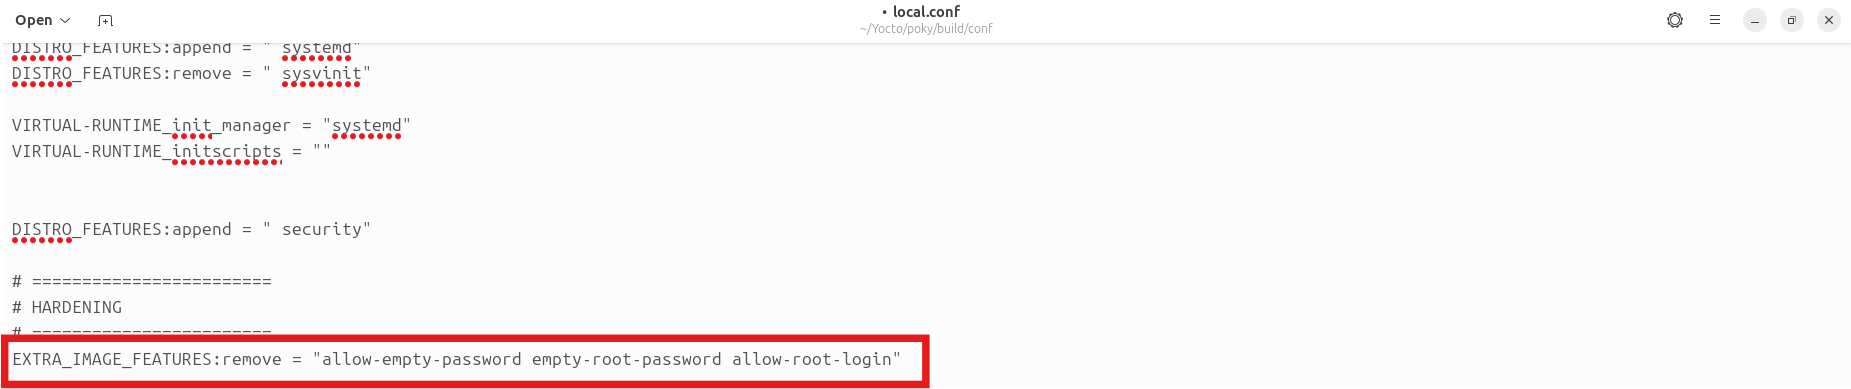
\includegraphics[width=1\textwidth]{image/gtbm.png}
    \caption{Giảm thiểu bề mặt tấn công trong Yocto Project}
    \label{fig:gtbm} 

\end{figure}

Để đảm bảo an toàn cho hệ thống, các lựa chọn “allow\-empty-password”, “allow\-root\-login” hoặc “empty\-root\-password” cần đảm bảo không phải là một trong những \texttt{IMAGE\_FEATURES}. 
Ngoài ra, chỉ giữ lại các thành phần thực sự cần thiết cho hệ thống Yocto thông qua các biến cấu hình như \texttt{DISTRO\_FEATURES} và  \texttt{IMAGE\_FEATURES}, nhằm giảm thiểu bề mặt tấn công. Bên cạnh đó, cần xem xét và tinh chỉnh cấu hình nhân hệ điều hành để đảm bảo chỉ bao gồm các trình điều khiển và tính năng cần thiết, tránh đưa vào những thành phần dư thừa có thể gây rủi ro bảo mật thông qua việc tùy chỉnh các thành phần trong kernel như \texttt{CONFIG\_DEVMEM} và \texttt{STRICT\_DEVMEM} nhằm hạn chế khả năng truy cập trực tiếp vào bộ nhớ thiết bị từ không gian người dùng. Điều này góp phần ngăn chặn các hành vi khai thác ở mức thấp, từ đó nâng cao mức độ an toàn tổng thể của hệ thống.

Một biện pháp quan trọng khác nhằm giảm thiểu rủi ro bị tấn công bề mặt là hạn chế hoặc không cho phép người dùng cài đặt thêm phần mềm sau khi thiết bị đã được triển khai. Trong các hệ thống sử dụng Yocto, phần mềm thường được build sẵn vào image, và hệ thống không được thiết kế như các bản phân phối Linux thông thường với trình quản lý gói mở cho người dùng. Việc cho phép cài đặt thêm package có thể làm mất kiểm soát cấu hình hệ thống, dẫn đến nguy cơ xuất hiện các phần mềm không được kiểm chứng hoặc chứa lỗ hổng bảo mật. Để giảm thiểu các rủi ro này, các developer không sử dụng các định dạng package như ipk, rpm hoặc deb trong quá trình build, đồng thời loại bỏ các thành phần package manager khỏi image. Ngoài ra, việc loại bỏ feature package-management và thiết lập hệ thống file ở chế độ chỉ đọc (read-only root filesystem) sẽ giúp ngăn chặn việc cài đặt hoặc thay đổi phần mềm trong quá trình vận hành.
Việc tinh chỉnh cấu hình kernel, loại bỏ các driver và tính năng không cần thiết, cũng như kích hoạt các tùy chọn bảo mật, giúp hạn chế khả năng khai thác từ các lỗ hổng mức thấp. Những biện pháp này góp phần xây dựng một hệ thống an toàn, ổn định và phù hợp với môi trường nhúng.



\subsection{Hiện thực Selinux}

Nhóm thực hiện bổ sung layer meta-selinux vào môi trường build:
\medskip

\begin{figure}[!h]
\renewcommand*\DTstyle{\ttfamily}
\dirtree{%
.1 meta-selinux/.
.2 classes/.
.2 conf/.
.2 recipes-core/.
.2 recipes-kernel/.
.2 recipes-security/.
.3 refpolicy/.
.3 selinux/.
.3 packagegroups/.
.3 images/.
.2 recipes-support/.
}
\caption{Cấu trúc thư mục chính của layer meta-selinux}
\label{fig:meta-selinux-structure}
\end{figure}
Hình \ref{fig:meta-selinux-structure} mô tả cấu trúc thư mục chính của layer \texttt{meta-selinux} trong Yocto Project. Layer này cung cấp các thành phần cần thiết để tích hợp cơ chế bảo mật SELinux vào hệ thống Linux nhúng. Trong đó, thư mục \texttt{classes} chứa các lớp hỗ trợ quá trình build và cấu hình SELinux; thư mục \texttt{conf} lưu trữ các thiết lập cấu hình của layer. Các thư mục \texttt{recipes-core}, \texttt{recipes-kernel} và \texttt{recipes-support} chứa các recipe bổ sung hoặc chỉnh sửa cho các thành phần hệ thống liên quan đến SELinux.

Đặc biệt, thư mục \texttt{recipes-security} đóng vai trò trung tâm trong việc triển khai cơ chế bảo mật. Bên trong thư mục này, \texttt{refpolicy} chứa các policy chuẩn của SELinux, \texttt{selinux} cung cấp các gói và công cụ hỗ trợ SELinux, \texttt{packagegroups} định nghĩa các nhóm package cần thiết, trong khi \texttt{images} hỗ trợ tích hợp SELinux trực tiếp vào image được build. Cấu trúc phân lớp này giúp việc quản lý, mở rộng và tùy chỉnh chính sách bảo mật trở nên linh hoạt và thuận tiện hơn trong quá trình phát triển hệ thống nhúng sử dụng Yocto Project.

SELinux hỗ trợ nhiều loại policy khác nhau nhằm đáp ứng các yêu cầu bảo mật và mức độ kiểm soát truy cập khác nhau của hệ thống. Trong đó, hai policy phổ biến nhất là \texttt{refpolicy-targeted} và \texttt{refpolicy-mls}. Mỗi policy được thiết kế cho các mục đích sử dụng riêng, từ các hệ thống Linux thông thường đến các môi trường yêu cầu bảo mật nghiêm ngặt. Việc lựa chọn policy phù hợp có ảnh hưởng trực tiếp đến mức độ bảo vệ, hiệu năng và độ phức tạp trong quá trình quản trị hệ thống.

\begin{table}[H]
\centering
\caption{So sánh các policy phổ biến của SELinux}
\label{tab:selinux-policy-comparison}

\renewcommand{\arraystretch}{1.4}

\begin{tabular}{|p{4cm}|p{3.5cm}|p{3cm}|p{4cm}|}
\hline
\textbf{Policy} & \textbf{Đặc điểm} & \textbf{Mức độ bảo mật} & \textbf{Trường hợp sử dụng} \\ \hline

\texttt{refpolicy-targeted}
&
Chỉ áp dụng cơ chế kiểm soát truy cập cho các tiến trình và dịch vụ quan trọng
&
Trung bình đến cao
&
Hệ thống nhúng, máy chủ thông thường, môi trường cần cân bằng giữa bảo mật và hiệu năng
\\ \hline

\texttt{refpolicy-mls}
&
Áp dụng cơ chế Multi-Level Security (MLS), kiểm soát truy cập theo nhiều cấp độ bảo mật
&
Rất cao
&
Hệ thống quân sự, chính phủ hoặc các môi trường yêu cầu phân cấp dữ liệu nghiêm ngặt
\\ \hline

\texttt{minimum}
&
Policy tối giản với số lượng rule hạn chế, chỉ bảo vệ các thành phần cơ bản
&
Cơ bản
&
Hệ thống tài nguyên hạn chế hoặc môi trường thử nghiệm
\\ \hline

\end{tabular}
\end{table}

Trong phạm vi đề tài, policy \texttt{refpolicy-targeted} được lựa chọn để triển khai trên hệ thống Yocto Linux. Nguyên nhân là do policy này cung cấp mức độ bảo mật phù hợp cho các hệ thống nhúng IoT nhưng vẫn đảm bảo tính ổn định và hiệu năng của hệ thống. So với \texttt{refpolicy-mls}, policy \texttt{targeted} có cấu hình đơn giản hơn, ít tiêu tốn tài nguyên và dễ triển khai trong môi trường thiết bị nhúng có giới hạn về bộ nhớ và năng lực xử lý. Đồng thời, policy này vẫn đủ khả năng bảo vệ các dịch vụ quan trọng khỏi các hành vi truy cập trái phép hoặc leo thang đặc quyền trong quá trình vận hành hệ thống.

Để tích hợp SELinux vào hệ thống Yocto, trước tiên cần bổ sung layer \texttt{meta-selinux} vào danh sách layer trong file \texttt{bblayers.conf}. Layer này cung cấp các recipe, policy và công cụ cần thiết để hỗ trợ cơ chế Mandatory Access Control (MAC) trên hệ thống Linux nhúng. Đồng thời, do \texttt{meta-selinux} phụ thuộc vào các layer từ repository \texttt{meta-openembedded}, bao gồm \texttt{meta-oe} và \texttt{meta-python}, các layer này cũng cần được thêm vào môi trường build để đảm bảo đầy đủ thư viện và thành phần hỗ trợ liên quan.

Sau khi thêm layer, hệ thống được cấu hình để kích hoạt SELinux thông qua việc bổ sung \texttt{selinux} vào biến \texttt{DISTRO\_FEATURES} trong file \texttt{local.conf}. Việc này giúp Yocto tự động tích hợp các thành phần SELinux vào image trong quá trình build. Ngoài ra, các package phụ trợ như \texttt{acl}, \texttt{xattr} và \texttt{pam} cũng được thêm vào nhằm đảm bảo SELinux có đầy đủ cơ chế quản lý quyền truy cập, extended attributes và xác thực người dùng.

\begin{figure}[!h]
    \centering
    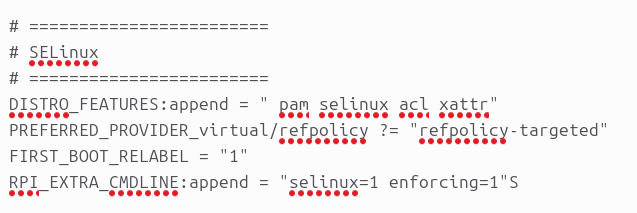
\includegraphics[width=0.7\textwidth]{image/selinuxx.png}
    \caption{Selinux}
    \label{fig:selinux} 
\end{figure}

Tiếp theo, hệ thống cần lựa chọn chính sách bảo mật phù hợp thông qua biến \texttt{PREFERRED\_}\\
\texttt{PROVIDER\_virtual/refpolicy} sử dụng policy \texttt{refpolicy-targeted}.


Sau khi hoàn tất các bước cấu hình, hệ thống được build lại để tạo ra image tích hợp SELinux. Trong quá trình vận hành, SELinux có thể hoạt động ở ba chế độ chính: enforcing, permissive và disabled. Ở chế độ enforcing, SELinux thực thi nghiêm ngặt các chính sách bảo mật, mọi hành vi truy cập không được phép sẽ bị chặn. Ở chế độ permissive, hệ thống không chặn các hành vi vi phạm mà chỉ ghi lại nhật ký, giúp nhà phát triển theo dõi và điều chỉnh chính sách phù hợp trong giai đoạn kiểm thử. Trong khi đó, chế độ disabled sẽ vô hiệu hóa hoàn toàn SELinux, hệ thống quay về cơ chế phân quyền truyền thống.
Việc kiểm tra trạng thái hoạt động của SELinux có thể được thực hiện thông qua các công cụ như getenforce hoặc sestatus. Thông qua đó, có thể xác định chế độ hiện tại của SELinux và đánh giá hiệu quả của các chính sách bảo mật đã được áp dụng trong hệ thống.

\subsection{Hiện thực dm-verity}

Quá trình triển khai dm-verity nhằm bảo vệ tính toàn vẹn của hệ thống được thực hiện qua các giai đoạn từ xây dựng hình ảnh hệ thống (\textit{system image}) tại môi trường phát triển cho đến quá trình thực thi kiểm chứng tại thiết bị đích. Cụ thể:

\subsubsection{Giai đoạn tiền xử lý và tách phân vùng dữ liệu}

Tiến trình bắt đầu bằng việc xây dựng image hệ thống gốc được đóng gói dưới định dạng \texttt{.wic}. Từ image này, phân vùng \textit{rootfs} tương ứng với phân vùng \texttt{p2} được tách riêng biệt để làm dữ liệu đầu vào cho quá trình tạo dữ liệu (\textit{metadata}) của dm-verity. Đây là bước then chốt nhằm đảm bảo toàn bộ thông tin băm (\textit{hash}) được sinh ra từ chính xác nội dung cuối cùng của \textit{rootfs} sau khi biên dịch, tạo sự đồng nhất tuyệt đối giữa dữ liệu tính toán và dữ liệu thực tế trên thiết bị.

\subsubsection{Khởi tạo cấu trúc cây băm (Hash Tree) và xác thực metadata}

Sử dụng công cụ \texttt{veritysetup}, hệ thống tiến hành chia phân vùng \texttt{p2} thành các khối dữ liệu (\textit{blocks}) có kích thước cố định. Tại đây, mỗi khối dữ liệu được xử lý qua thuật toán băm SHA-256 để tạo ra các giá trị băm tương ứng. Các giá trị này được tổ chức theo cấu trúc cây băm nhiều mức (\textit{Merkle Tree}), dẫn đến hai thành phần đầu ra quan trọng:

\begin{itemize}
    \item \texttt{rootfs.hash}: tệp tin chứa toàn bộ cấu trúc cây băm của phân vùng.
    \begin{figure}[!h]
    \centering
    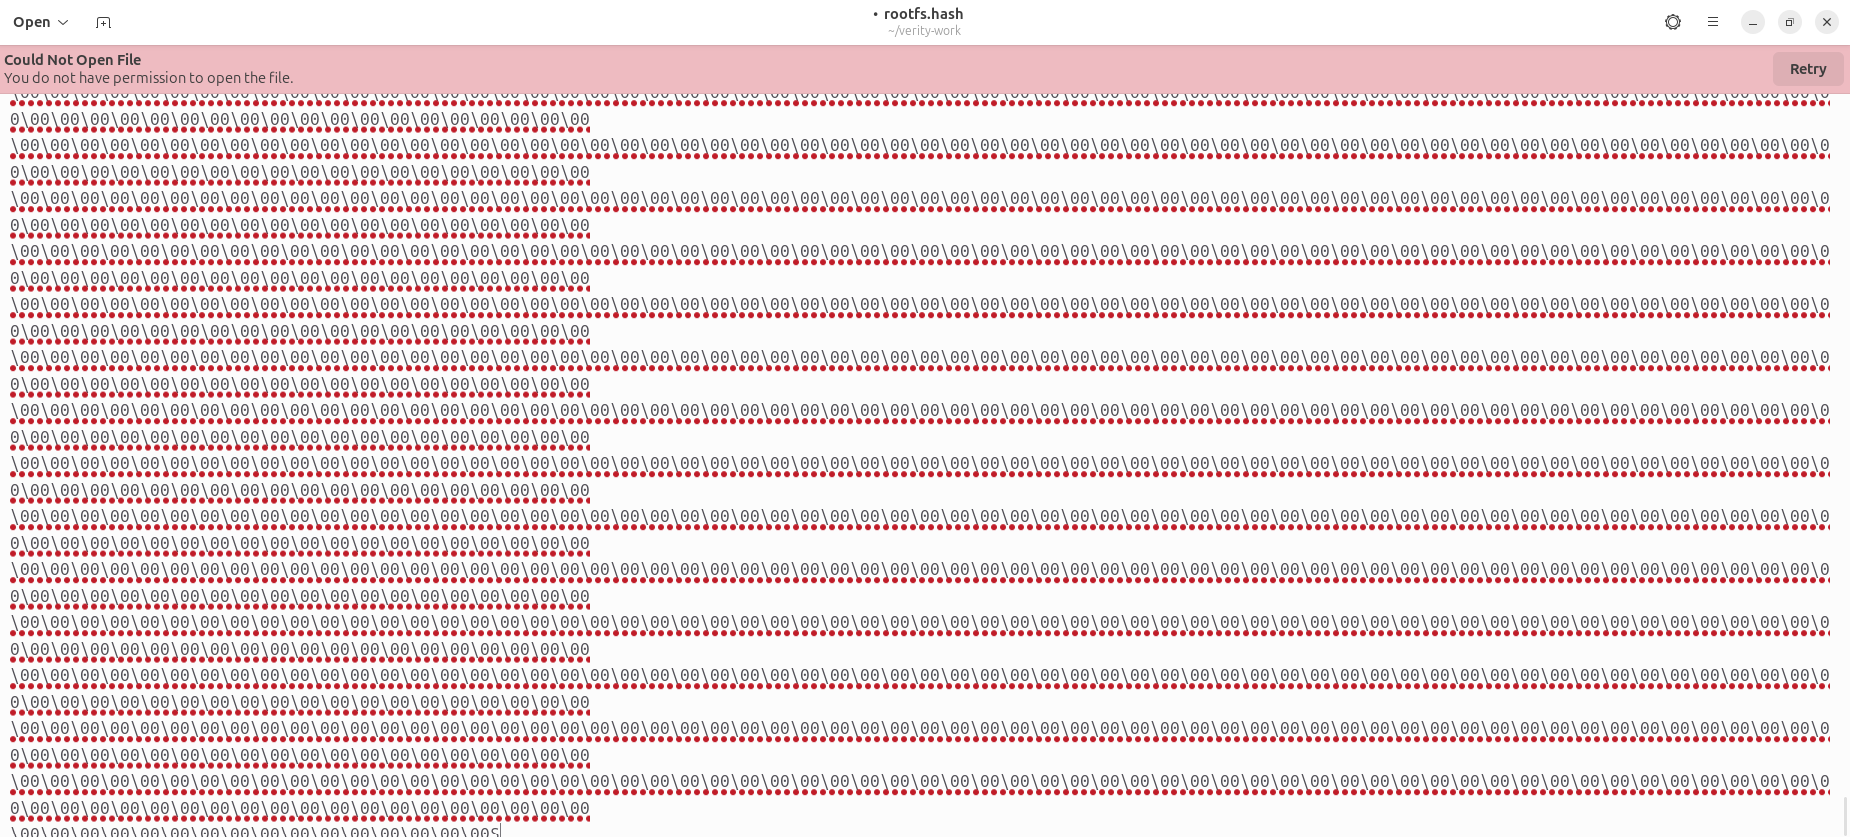
\includegraphics[width=1\textwidth]{image/roothash.png}
    \caption{Cấu trúc cây băm của rootfs}
    \label{fig:roothash} 
\end{figure}

    \item \texttt{root.hash}: giá trị băm gốc (\textit{root hash}), đại diện duy nhất cho tính toàn vẹn của toàn bộ phân vùng \textit{rootfs}.
\begin{figure}[!h]
    \centering
    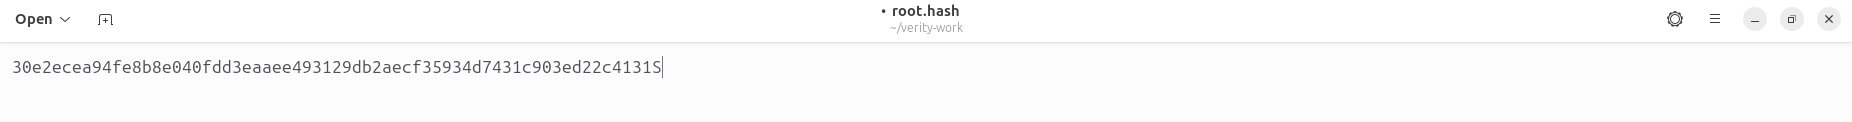
\includegraphics[width=1\textwidth]{image/root.png}
    \caption{Giá trị băm gốc (root hash)}
    \label{fig:rootkey} 
\end{figure}

  \end{itemize}

Để đảm bảo độ tin cậy, lệnh \texttt{veritysetup verify} được thực thi nhằm kiểm tra tính nhất quán giữa dữ liệu gốc và các thành phần \textit{metadata} vừa khởi tạo trước khi tiến hành nạp vào thiết bị.
\begin{figure}[!h]
    \centering
    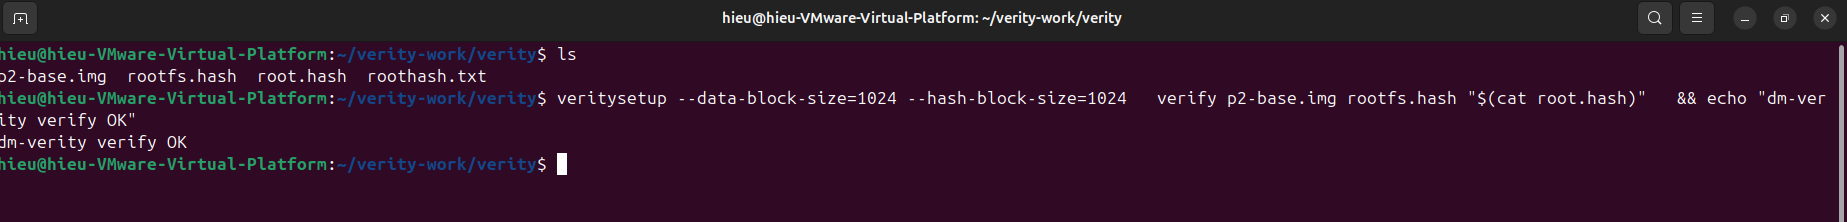
\includegraphics[width=1\textwidth]{image/verityok.png}
    \caption{Kết quả xác thực metadata của dm-verity}
    \label{fig:verityok} 
\end{figure}

\subsubsection{Triển khai và cấu hình giai đoạn khởi động sớm}

Sau khi xác thực thành công, hình ảnh hệ thống được nạp vào thẻ nhớ SD. Trong cấu trúc này, phân vùng \texttt{p1} đảm nhiệm vai trò khởi động (\textit{boot partition}), trong khi \texttt{p2} chứa \textit{rootfs} cần được bảo vệ. Các tệp tin \texttt{root.hash} và \texttt{rootfs.hash} được lưu trữ vào thư mục \texttt{/verity} trên phân vùng \texttt{p1}, cho phép hệ thống tệp trong bộ nhớ tạm (\textit{initramfs}) có thể truy xuất trong giai đoạn khởi động sớm.

\subsubsection{Cơ chế kiểm chứng thực thi tại thiết bị đích}

Tại thiết bị đích, tiến trình khởi động được điều khiển bởi Kernel và \textit{initramfs}. Tập lệnh \texttt{/init} trong \textit{initramfs} thực hiện gắn kết (\textit{mount}) phân vùng boot \texttt{p1}, truy xuất các tệp tin băm và sử dụng lệnh \texttt{veritysetup open} để thiết lập một thiết bị ánh xạ (\textit{mapping device}) cho phân vùng \texttt{p2}. Lớp ánh xạ này đóng vai trò là một tầng trung gian kiểm soát giữa hệ điều hành và dữ liệu vật lý.
Nội dung của file \texttt{/init} được trình bày dưới đây:\\
\begin{lstlisting}[style=thesisstyle, language=bash]
#!/bin/sh

export PATH=/sbin:/bin:/usr/sbin:/usr/bin

panic() {
    echo "INITRAMFS ERROR: $*" > /dev/console
    exec sh
}

echo "Starting dm-verity initramfs..." > /dev/console

# Mount filesystem
mount -t proc proc /proc || panic "mount proc failed"
mount -t sysfs sysfs /sys || panic "mount sys failed"
mount -t devtmpfs devtmpfs /dev || panic "mount dev failed"

# Load module
modprobe dm_mod
modprobe dm_verity
modprobe loop
modprobe ext4
modprobe vfat

# Tao thu muc chua file hash
mkdir -p /mnt/boot /newroot

# Mount boot partition
mount -t vfat -o ro /dev/mmcblk0p1 /mnt/boot \
    || panic "boot mount failed"

# Gan file hash vao loop device
losetup -r /dev/loop0 /mnt/boot/rootfs.hash \
    || panic "loop setup failed"

# Kich hoat dm-verity
veritysetup open /dev/mmcblk0p2 vroot /dev/loop0 \
    --root-hash-file /etc/verity/root.hash \
    || panic "verity open failed"

# Mount verified rootfs
mount -t ext4 -o ro /dev/mapper/vroot /newroot \
    || panic "rootfs mount failed"

# Chuyen sang rootfs that
exec switch_root /newroot /sbin/init
\end{lstlisting}

File \texttt{init} trong \texttt{initramfs} có vai trò khởi tạo môi trường tối thiểu trước khi hệ điều hành chuyển sang \textit{root filesystem} chính đã được bảo vệ bằng cơ chế \texttt{dm-verity}. Đầu tiên, script tiến hành mount các filesystem cần thiết như \texttt{/proc}, \texttt{/sys} và \texttt{/dev} để cung cấp môi trường hoạt động cơ bản cho kernel và userspace. Sau đó, các kernel module liên quan như \texttt{dm\_mod}, \texttt{dm\_verity}, \texttt{loop}, \texttt{ext4} và \texttt{vfat} được nạp để hỗ trợ cơ chế xác thực filesystem và mount các phân vùng lưu trữ.

Tiếp theo, script mount phân vùng boot ở chế độ chỉ đọc để truy cập file \texttt{rootfs.hash}, đây là Merkle Hash Tree dùng cho cơ chế xác thực toàn vẹn dữ liệu. File hash này được ánh xạ vào loop device thông qua \texttt{losetup}, cho phép \texttt{dm-verity} sử dụng như một block device phục vụ quá trình kiểm tra integrity. Sau đó, lệnh \texttt{veritysetup open} được sử dụng để tạo thiết bị ánh xạ \texttt{/dev/mapper/vroot}. Từ thời điểm này, mọi block dữ liệu được đọc từ root filesystem sẽ được kernel tự động kiểm tra hash nhằm phát hiện các thay đổi trái phép.

Sau khi quá trình xác thực thành công, root filesystem đã được bảo vệ sẽ được mount ở chế độ chỉ đọc vào thư mục \texttt{/newroot}. Cuối cùng, lệnh \texttt{switch\_root} được thực thi để chuyển quyền điều khiển sang hệ thống chính và tiếp tục quá trình khởi động Linux thông qua \texttt{/sbin/init}.

Mọi yêu cầu truy cập dữ liệu từ \textit{rootfs} sẽ được đối chiếu theo thời gian thực với cấu trúc cây băm và giá trị băm gốc đã thiết lập.

\begin{itemize}
    \item \textbf{Trường hợp dữ liệu hợp lệ:} Nếu dữ liệu trên \texttt{p2} hoàn toàn khớp với \textit{metadata}, hệ thống sẽ tiến hành gắn kết \textit{rootfs} ở chế độ chỉ đọc (\textit{read-only}) và thực hiện lệnh \texttt{switch\_root} để chuyển sang hệ điều hành chính thức.
    
    \item \textbf{Trường hợp dữ liệu bị can thiệp:} Nếu xuất hiện bất kỳ sự sai lệch nào giữa dữ liệu thực tế và cây băm, dm-verity sẽ ngay lập tức phát hiện, từ chối quyền truy cập và ngăn chặn quá trình gắn kết hệ thống. Lúc này, thiết bị sẽ chuyển sang trạng thái lỗi hoặc chế độ phục hồi (\textit{recovery mode}).
\end{itemize}

\section{Hiện thực Device Driver}

\subsection{Tổng quan kiến trúc Driver}
Trong hệ thống, nhóm triển khai hai device driver chính bao gồm driver giao tiếp I2C và driver giao tiếp RS485 Modbus RTU trên nền tảng Linux nhúng Yocto. Các driver này đóng vai trò trung gian giữa tầng ứng dụng (user space) và phần cứng ngoại vi.

Driver được hiện thực dưới dạng character device driver, cho phép các ứng dụng user space có thể giao tiếp với phần cứng thông qua các device file trong thư mục \texttt{/dev}. Việc tự xây dựng driver giúp hệ thống có tính tùy biến cao, đồng thời hỗ trợ tối ưu cho các ứng dụng tự động hóa công nghiệp.

Kiến trúc tổng quát của hệ thống driver được mô tả như sau:

\begin{center}
User Application $\rightarrow$ Device Driver $\rightarrow$ Hardware Interface $\rightarrow$ Peripheral Device
\end{center}


\subsection{Hiện thực driver I2C}

Trong đề tài, nhóm xây dựng một driver I2C dạng software bit-banging trên nền tảng Linux nhúng Yocto nhằm hỗ trợ giao tiếp với các thiết bị ngoại vi như màn hình OLED SSD1306 và các cảm biến môi trường. Driver được hiện thực dưới dạng character device driver cho phép ứng dụng ở user space có thể giao tiếp với phần cứng thông qua device file trong thư mục \texttt{/dev}.

Khác với việc sử dụng bộ điều khiển I2C phần cứng mặc định của Raspberry Pi 4, nhóm lựa chọn hiện thực giao thức I2C bằng phần mềm thông qua GPIO nhằm tăng tính tùy biến và chủ động trong việc điều khiển giao thức. Cách tiếp cận này cho phép hệ thống dễ dàng thay đổi chân SDA và SCL trong quá trình runtime, đồng thời hỗ trợ nghiên cứu cơ chế hoạt động của giao thức I2C ở mức thấp trong Linux kernel.

\subsubsection{Kiến trúc driver}

Driver được xây dựng theo mô hình character device driver của Linux kernel. Sau khi module được nạp vào hệ thống, driver sẽ đăng ký major number và tạo device file \texttt{/dev/my\_i2c\_soft} để các ứng dụng user space có thể truy cập.
Luồng hoạt động của driver được mô tả như sau:

\begin{center}
User Application $\rightarrow$ Character Device Driver $\rightarrow$ GPIO Bit-banging $\rightarrow$ I2C Device
\end{center}

Trong mô hình này, tầng user application gửi dữ liệu xuống kernel thông qua các system call như \texttt{read()}, \texttt{write()} và \texttt{ioctl()}. Driver sẽ xử lý dữ liệu và điều khiển trực tiếp các chân GPIO để tạo tín hiệu SDA và SCL theo chuẩn giao thức I2C.

\subsubsection{Nguyên lý giao thức I2C}

Giao thức I2C sử dụng hai đường tín hiệu bao gồm SDA (Serial Data) và SCL (Serial Clock). Quá trình truyền dữ liệu được đồng bộ bằng xung clock từ master device.
Driver sử dụng cơ chế điều khiển trực tiếp GPIO để mô phỏng giao thức I2C thông qua phương pháp bit-banging.
Trong driver, nhóm hiện thực các tín hiệu cơ bản của giao thức I2C bao gồm:

\begin{itemize}
    \item START condition.
    \item STOP condition.
    \item Truyền dữ liệu theo từng bit.
    \item Nhận ACK từ slave device.
    \item Đọc dữ liệu từ slave.
\end{itemize}

\subsubsection{Các chức năng chính của driver}

Driver I2C Software được xây dựng nhằm mô phỏng cơ chế giao tiếp I2C thông qua điều khiển GPIO bằng phần mềm trong Linux Kernel. Để đảm bảo tín hiệu giao tiếp ổn định và đáp ứng đúng yêu cầu timing của giao thức I2C, driver sử dụng hàm \texttt{udelay()} để tạo các khoảng trễ ngắn giữa các cạnh xung clock trong quá trình truyền nhận dữ liệu.

Trong quá trình hoạt động, driver đảm nhiệm nhiều chức năng quan trọng liên quan đến điều khiển bus I2C và giao tiếp giữa kernel space với user space. Các chức năng chính của driver bao gồm:

\begin{itemize}
    \item Khởi tạo, cấu hình và giải phóng các chân GPIO được sử dụng cho hai tín hiệu SDA và SCL.
    
    \item Hiện thực cơ chế tạo tín hiệu START và STOP theo đúng chuẩn giao thức I2C nhằm bắt đầu và kết thúc quá trình truyền dữ liệu.
    
    \item Hỗ trợ cơ chế truyền và nhận dữ liệu theo từng byte thông qua quá trình điều khiển tín hiệu clock và data bằng phần mềm.
    
    \item Kiểm tra và xử lý tín hiệu ACK từ slave device sau mỗi lần truyền dữ liệu nhằm đảm bảo tính chính xác của quá trình giao tiếp.
    
    \item Cung cấp khả năng đọc và ghi dữ liệu từ user space thông qua các system call như \texttt{read()} và \texttt{write()}.
    
    \item Hỗ trợ cấu hình động các chân GPIO và địa chỉ slave device thông qua cơ chế \texttt{ioctl()}, giúp tăng tính linh hoạt trong quá trình sử dụng driver.
\end{itemize}

Thông qua các chức năng trên, driver cho phép hệ thống Linux nhúng thực hiện giao tiếp với các thiết bị ngoại vi I2C mà không phụ thuộc hoàn toàn vào phần cứng I2C controller tích hợp sẵn trên vi xử lý. Điều này giúp tăng tính linh hoạt trong quá trình phát triển và kiểm thử các hệ thống nhúng sử dụng Linux Kernel.

\subsubsection{Thiết kế cơ chế IOCTL}

Driver sử dụng cơ chế \texttt{ioctl()} để cho phép ứng dụng user space cấu hình động chân SDA, SCL và địa chỉ slave device trong quá trình runtime.
Các IOCTL command được định nghĩa như sau:

\begin{lstlisting}[style=thesisstyle, language=C]
#define SET_SDA_PIN    _IOW(I2C_IOCTL_MAGIC, 1, int)
#define SET_SCL_PIN    _IOW(I2C_IOCTL_MAGIC, 2, int)
#define SET_SLAVE_ADDR _IOW(I2C_IOCTL_MAGIC, 3, int)
\end{lstlisting}

Cách tiếp cận này giúp hệ thống có khả năng thay đổi cấu hình GPIO linh hoạt mà không cần biên dịch lại kernel module.

\subsubsection{Giao tiếp giữa user space và kernel space}

Driver sử dụng cấu trúc \texttt{file\_operations} để đăng ký các system call với Linux kernel.

\begin{lstlisting}[style=thesisstyle, language=C]
static struct file_operations fops = {
    .unlocked_ioctl = my_ioctl,
    .write = dev_write,
    .read = dev_read,
    .owner = THIS_MODULE,
};
\end{lstlisting}

Thông qua cơ chế này, ứng dụng user space có thể sử dụng các system call chuẩn của Linux để giao tiếp với driver.

\subsubsection{Hiện thực giao thức I2C bằng GPIO Bit-banging}

Driver hiện thực các tín hiệu cơ bản của giao thức I2C thông qua việc điều khiển trực tiếp GPIO. Tín hiệu START được hiện thực như sau:

\begin{lstlisting}[style=thesisstyle, language=C]
static void i2c_start(void) {
    gpio_direction_output(current_sda, 1);

    gpio_set_value(current_scl, 1);
    udelay(I2C_DELAY);

    gpio_set_value(current_sda, 0);
    udelay(I2C_DELAY);

    gpio_set_value(current_scl, 0);
    udelay(I2C_DELAY);
}
\end{lstlisting}

Ngoài ra, driver còn hỗ trợ cơ chế ACK và đọc dữ liệu từ slave device nhằm đảm bảo khả năng giao tiếp hai chiều.

\subsubsection{Tối ưu timing cho giao tiếp I2C}

Trong quá trình thử nghiệm với màn hình OLED SSD1306, nhóm nhận thấy timing không ổn định có thể gây lỗi hiển thị và tạo ra hiện tượng nhiễu dữ liệu.
Do đó, driver được tinh chỉnh delay giữa các cạnh clock bằng hàm \texttt{udelay()} nhằm đảm bảo thời gian setup và hold của dữ liệu trước khi phát xung clock.
Trong quá trình truyền dữ liệu, driver sử dụng delay ngắn trước và sau cạnh clock để tăng độ ổn định:

\begin{lstlisting}[style=thesisstyle, language=C]
gpio_set_value(current_scl, 0);

udelay(I2C_DELAY / 2);

gpio_set_value(current_sda, (byte >> i) & 1);

udelay(I2C_DELAY / 2);

gpio_set_value(current_scl, 1);

udelay(I2C_DELAY);
\end{lstlisting}

Việc tối ưu timing giúp cải thiện độ ổn định khi hiển thị dữ liệu trên OLED và giảm lỗi truyền nhận dữ liệu trong quá trình giao tiếp.

\subsubsection{Tích hợp driver vào hệ thống Yocto}

Driver được tích hợp vào hệ thống Yocto thông qua custom layer \texttt{meta-i2c}. Nhóm xây dựng recipe BitBake nhằm tự động hóa quá trình build và đóng gói kernel module.
Cấu trúc layer của driver được tổ chức như sau:

\medskip 

\renewcommand*\DTstyle{\ttfamily} 
\dirtree{%
.1 meta-i2c/.
.2 conf/.
.3 layer.conf.
.2 recipes-kernel/.
.3 i2c-driver/.
.4 files/.
.5 my\_i2c\_soft.c.
.5 Makefile.
.4 i2c-soft-driver.bb.
}

Recipe của driver kế thừa lớp \texttt{module} nhằm hỗ trợ build kernel module trên Yocto:

\begin{lstlisting}[style=thesisstyle, language=C]
SUMMARY = "Dynamic Software I2C Driver"

inherit module

SRC_URI = "file://my_i2c_soft.c \
           file://Makefile"

KERNEL_MODULE_AUTOLOAD += "my_i2c_soft"
\end{lstlisting}

Yocto hỗ trợ cơ chế tự động nạp kernel module khi hệ thống khởi động thông qua biến:

\begin{verbatim}
KERNEL_MODULE_AUTOLOAD += "my_i2c_soft"
\end{verbatim}


Khi build image Yocto, kernel module sẽ được tích hợp vào hệ thống dưới dạng file \texttt{.ko} và có thể tự động nạp khi khởi động.
Layer chứa driver được tích hợp vào môi trường build của Yocto thông qua lệnh:

\begin{verbatim}
bitbake-layers add-layer ../meta-i2c
\end{verbatim}

Sau khi layer được thêm vào hệ thống, BitBake sẽ tự động quét và phân tích các recipe, configuration và metadata bên trong layer. Các recipe này sau đó được đưa vào dependency graph của quá trình build nhằm phục vụ việc biên dịch và tích hợp driver vào hệ thống Linux Embedded.

Để driver được đưa vào image cuối cùng, hệ thống sử dụng biến:

\begin{verbatim}
IMAGE_INSTALL:append = "my_i2c_soft"
\end{verbatim}

Biến này cho phép package của driver được tự động tích hợp vào root filesystem trong quá trình build image. Nhờ đó, hệ thống Linux Embedded sau khi boot sẽ có đầy đủ kernel module và các thành phần cần thiết phục vụ quá trình runtime.

Khi image được build, Yocto sẽ tự động sinh các cấu hình cần thiết trong thư mục \texttt{/etc/modules-load.d/}, cho phép Linux Kernel tự động nạp module trong quá trình boot hệ thống. Cơ chế này giúp driver luôn sẵn sàng hoạt động ngay sau khi thiết bị khởi động mà không cần thao tác nạp module thủ công.

Sau khi hệ thống khởi động, kernel module có thể được kiểm tra thông qua các lệnh quản lý module của Linux. Một số lệnh phổ biến được trình bày trong Bảng \ref{tab:runtime_verify_commands}.


\subsection{Hiện thực Driver RS485 Modbus RTU}

\subsubsection{Kiến trúc Driver}

Driver RS485 được xây dựng dưới dạng Linux Kernel Module nhằm phục vụ giao tiếp giữa hệ thống Linux Embedded và cảm biến môi trường thông qua giao thức Modbus RTU trên nền UART. Driver được thiết kế theo mô hình phân lớp của Linux Kernel, trong đó tầng Character Device đóng vai trò giao tiếp với User Space, còn tầng Serdev đảm nhiệm việc truyền nhận dữ liệu UART với phần cứng.

Kiến trúc tổng thể của driver được mô tả như sau:

\[
\begin{array}{c}
\text{User Space Application} \\
\downarrow \\
\text{Character Device (/dev/sensorhub)} \\
\downarrow \\
\text{RS485 Kernel Module} \\
\downarrow \\
\text{Serdev Framework} \\
\downarrow \\
\text{UART1 / ttyS0} \\
\downarrow \\
\text{RS485 Transceiver} \\
\downarrow \\
\text{Modbus Sensor}
\end{array}
\]

Trong kiến trúc này, ứng dụng ở User Space có thể truy cập dữ liệu cảm biến thông qua device file \texttt{/dev/sensorhub}. Driver sử dụng Serdev Framework của Linux Kernel để quản lý giao tiếp UART thay cho cơ chế platform driver truyền thống. Cách tiếp cận này giúp giảm mức độ phụ thuộc phần cứng và tăng khả năng tích hợp trong các hệ thống Linux Embedded hiện đại.

Driver được tổ chức thành nhiều thành phần mã nguồn độc lập bao gồm:
\begin{itemize}
    \item \texttt{rs485\_modbus.c}: hiện thực Character Device và cơ chế polling dữ liệu cảm biến.
    
    \item \texttt{rs485\_rtu.c}: hiện thực giao thức Modbus RTU và cơ chế truyền nhận UART.
    
    \item \texttt{rs485\_modbus.h}: khai báo cấu trúc dữ liệu, macro và tài nguyên dùng chung.
\end{itemize}

Việc tách driver thành nhiều thành phần giúp mã nguồn dễ bảo trì, thuận lợi cho việc mở rộng chức năng và nâng cao khả năng tái sử dụng trong các hệ thống khác nhau.

\subsubsection{Nguyên lý giao thức}

Driver sử dụng giao thức Modbus RTU để giao tiếp với cảm biến môi trường thông qua chuẩn truyền thông RS485. Trong cơ chế này, Raspberry Pi 4 đóng vai trò Master, còn cảm biến hoạt động như Slave Device với địa chỉ mặc định là \texttt{0x15}.

Khung dữ liệu Modbus RTU được xây dựng theo cấu trúc:

\begin{center}
\begin{verbatim}
| Slave Address | Function Code | Data | CRC16 |
\end{verbatim}
\end{center}

Trong đó:
\begin{itemize}
    \item \textbf{Slave Address}: địa chỉ thiết bị Modbus.
    
    \item \textbf{Function Code}: mã chức năng truy cập thanh ghi.
    
    \item \textbf{Data}: dữ liệu thanh ghi cần đọc hoặc ghi.
    
    \item \textbf{CRC16}: giá trị kiểm tra lỗi truyền thông.
\end{itemize}

Driver hỗ trợ các mã chức năng Modbus phổ biến bao gồm:
\begin{itemize}
    \item \texttt{0x03}: đọc Holding Registers.
    
    \item \texttt{0x04}: đọc Input Registers.
    
    \item \texttt{0x06}: ghi Single Register.
\end{itemize}

Các giá trị cảm biến được đọc từ vùng thanh ghi Modbus và chuyển đổi sang cấu trúc dữ liệu nội bộ của driver. Để đảm bảo tính ổn định trong Linux Kernel, các giá trị nhiệt độ, độ ẩm và áp suất được biểu diễn dưới dạng fixed-point thay cho floating-point.

\subsubsection{Các chức năng chính của Driver}

Driver được xây dựng nhằm đảm bảo quá trình giao tiếp giữa hệ thống Linux Embedded và cảm biến RS485 diễn ra ổn định, đồng thời cung cấp cơ chế truy cập dữ liệu thuận tiện cho các ứng dụng ở User Space. Trong quá trình hoạt động, driver đảm nhiệm nhiều chức năng khác nhau, từ quản lý giao tiếp UART cho đến xử lý dữ liệu Modbus RTU và đồng bộ tài nguyên trong Kernel Space.

Về mặt truyền thông, driver sử dụng Serdev Framework của Linux Kernel để khởi tạo và quản lý giao tiếp UART với thiết bị RS485. Thông qua cơ chế này, driver có thể điều khiển tín hiệu DE/RE của transceiver nhằm chuyển đổi linh hoạt giữa chế độ truyền và nhận dữ liệu trên đường truyền RS485. Bên cạnh đó, driver còn thực hiện việc xây dựng khung dữ liệu Modbus RTU, gửi request đến cảm biến và tiếp nhận phản hồi từ slave device theo đúng chuẩn giao thức.

Trong quá trình truyền nhận dữ liệu, driver triển khai cơ chế kiểm tra CRC16 để phát hiện lỗi truyền thông và đảm bảo tính toàn vẹn của dữ liệu nhận được. Sau khi khung dữ liệu hợp lệ được xác nhận, các giá trị thanh ghi Modbus sẽ được giải mã và chuyển đổi sang định dạng dữ liệu nội bộ của hệ thống. Driver hỗ trợ thu thập dữ liệu cảm biến theo chu kỳ định sẵn thông qua kernel thread, cho phép hệ thống cập nhật trạng thái môi trường một cách liên tục trong thời gian thực.

Ngoài chức năng giao tiếp phần cứng, driver còn cung cấp Character Device để các ứng dụng ở User Space có thể truy cập dữ liệu cảm biến thông qua các system call chuẩn của Linux như \texttt{open()}, \texttt{read()} và \texttt{ioctl()}. Để đảm bảo tính ổn định trong môi trường đa tiến trình, driver sử dụng nhiều cơ chế đồng bộ của Linux Kernel như \texttt{mutex}, \texttt{spinlock} và \texttt{completion} nhằm bảo vệ vùng dữ liệu dùng chung và hạn chế race condition trong quá trình truy cập tài nguyên.

Dữ liệu cảm biến sau khi giải mã được lưu trữ trong cấu trúc \texttt{sensor\_data} như sau:

\begin{lstlisting}[style=thesisstyle, language=C]
struct sensor_data {
    u32 humidity;
    s32 temperature;
    u32 pm25;
    u32 pressure;
    u32 lux;
};
\end{lstlisting}

Cấu trúc này đóng vai trò như vùng dữ liệu trung gian giữa Kernel Space và User Space. Các giá trị cảm biến sau khi được cập nhật từ quá trình polling sẽ được lưu vào bộ nhớ đệm nội bộ của driver trước khi chuyển đến ứng dụng người dùng thông qua Character Device. Cách tổ chức này giúp giảm số lần truy cập trực tiếp đến phần cứng, đồng thời nâng cao tính ổn định và hiệu năng của hệ thống trong quá trình vận hành.
\subsubsection{Thiết kế cơ chế hoạt động}

Driver triển khai cơ chế polling định kỳ nhằm tự động cập nhật dữ liệu cảm biến trong thời gian thực. Một kernel thread riêng biệt được tạo ra để thực hiện chu trình truyền nhận Modbus liên tục.

Quy trình hoạt động của driver được mô tả như sau:

\[
\begin{array}{c}
\text{Kernel Thread} \\
\downarrow \\
\text{Send Modbus Request} \\
\downarrow \\
\text{UART Transmission} \\
\downarrow \\
\text{Receive Response} \\
\downarrow \\
\text{CRC Verification} \\
\downarrow \\
\text{Decode Registers} \\
\downarrow \\
\text{Update Cache} \\
\downarrow \\
\text{Expose to User Space}
\end{array}
\]

Trong quá trình hoạt động, driver sử dụng:
\begin{itemize}
    \item \texttt{mutex}: đồng bộ truy cập dữ liệu cache.
    
    \item \texttt{spinlock}: bảo vệ vùng dữ liệu RX trong interrupt context.
    
    \item \texttt{completion}: đồng bộ cơ chế chờ phản hồi UART.
\end{itemize}

Cơ chế này giúp driver hoạt động ổn định trong môi trường đa tiến trình của Linux Kernel và hạn chế lỗi race condition trong quá trình truyền nhận dữ liệu.

\subsubsection{Tích hợp Driver vào hệ thống Yocto}

Driver được đóng gói dưới dạng một custom layer trong Yocto Project nhằm phục vụ quá trình build Embedded Linux Image.

Cấu trúc layer được tổ chức như sau:

\medskip 

\renewcommand*\DTstyle{\ttfamily} 
\dirtree{%
.1 meta-rs485/.
.2 conf/.
.3 layer.conf.
.2 recipes-kernel/.
.3 rs485-driver/.
.4 files/.
.5 rs485\_modbus.c.
.5 rs485\_modbus.h.
.5 rs485\_rtu.c.
.5 rs485\_rtu.h.
.5 rs485-pi4.dts.
.5 rs485-pi4.dtbo.
.5 Makefile.
.4 rs485-driver.bb.
}

Layer được tích hợp vào môi trường build bằng lệnh:

\begin{verbatim}
bitbake-layers add-layer ../meta-rs485
\end{verbatim}

Sau khi layer được thêm vào hệ thống, BitBake sẽ tự động quét recipe và metadata của driver để đưa vào dependency graph của quá trình build.
Driver được tích hợp vào Embedded Linux Image thông qua biến:

\begin{verbatim}
IMAGE_INSTALL:append = " rs485-driver"
\end{verbatim}

Biến này cho phép package của driver được tự động đưa vào root filesystem trong quá trình build image.
Bên cạnh đó, hệ thống còn hỗ trợ cơ chế tự động nạp kernel module khi boot thông qua biến, Cơ chế này giúp module được tự động nạp khi hệ thống khởi động mà không cần thao tác thủ công từ người dùng:

\begin{verbatim}
KERNEL_MODULE_AUTOLOAD += "rs485_sensor_mod"
\end{verbatim}

Driver cũng sử dụng Device Tree Overlay để mô tả phần cứng UART và thiết bị RS485 trong hệ thống Raspberry Pi 4. Device Tree được định nghĩa trong file \texttt{rs485-pi4.dts} và biên dịch thành file overlay nhị phân \texttt{.dtbo}.

Một đoạn cấu hình Device Tree tiêu biểu được trình bày như sau:

\begin{lstlisting}[style=thesisstyle, language=C]
rs485sensor@15 {
    compatible = "mycompany,rs485-sensorhub";
    reg = <0x15>;
    current-speed = <9600>;
};
\end{lstlisting}

Sau khi biên dịch, file \texttt{.dtbo} sẽ được cài đặt vào thư mục:

\begin{verbatim}
/boot/overlays/
\end{verbatim}

Linux Kernel sử dụng Device Tree Overlay để nhận diện phần cứng và thực hiện binding giữa driver với thiết bị UART tương ứng trong quá trình boot hệ thống.

\section{Hiện thực Khối xử lý AI}

Phần này mô tả quá trình chuyển đổi các thiết kế lý thuyết thành hệ thống phần mềm thực tế, bao gồm từ bước chuẩn bị dữ liệu, xây dựng cấu trúc mạng đến việc tối ưu hóa để triển khai trên phần cứng Raspberry Pi 4.

\subsection{Thiết lập môi trường và Công cụ hỗ trợ}

Toàn bộ khối xử lý AI được hiện thực bằng ngôn ngữ lập trình Python 3.10 trên môi trường máy trạm (Workstation) để tận dụng khả năng tính toán của GPU trong quá trình huấn luyện.

\begin{itemize}
    \item \textbf{TensorFlow \& Keras (v2.15+):} Nền tảng chính để xây dựng các lớp mạng nơ-ron.
    
    \item \textbf{Keras-TCN:} Thư viện mã nguồn mở chuyên biệt để triển khai các khối Temporal Convolutional Network (TCN).
    
    \item \textbf{Pandas \& NumPy:} Sử dụng để cấu trúc hóa dữ liệu từ tệp CSV và thực hiện các phép toán ma trận trên mảng đa chiều.
    
    \item \textbf{Scikit-learn:} Cung cấp module \texttt{MinMaxScaler} để chuẩn hóa dữ liệu và các hàm đo lường hiệu năng.
\end{itemize}

\subsection{Hiện thực Tiền xử lý và Cấu trúc hóa Dữ liệu}

Dữ liệu thô từ trạm cảm biến môi trường (bao gồm $r$ thông số) cần được xử lý để loại bỏ nhiễu và định dạng lại thành cấu trúc chuỗi thời gian (\textit{time-series}).

\subsubsection{Làm mượt và Chuẩn hóa dữ liệu}

Để giảm thiểu tác động của các giá trị nhiễu tức thời (\textit{spikes}), hệ thống hiện thực kỹ thuật trung bình trượt (\textit{rolling mean}) với cửa sổ bằng 10 bước thời gian. Sau đó, dữ liệu được đưa về khoảng $[0,1]$ bằng phương pháp Min-Max Scaling nhằm tăng tốc độ hội tụ của thuật toán tối ưu Adam.

\begin{lstlisting}[style=thesisstyle, language=Python]
# Lam muot du lieu PM2.5 va Sound
df['pm2p5'] = df['pm2p5'].rolling(window=10).mean().bfill()
df['sound'] = df['sound'].rolling(window=10).mean().bfill()

# Chuan hoa Min-Max
scaler = MinMaxScaler()
scaled_data = scaler.fit_transform(df)
\end{lstlisting}

\subsubsection{Cấu trúc cửa sổ trượt (Sliding Window)}

Hàm \texttt{create\_dataset()} được hiện thực để chuyển đổi mảng dữ liệu hai chiều thành mảng ba chiều có dạng:

\[
(samples,\; time\_steps,\; features)
\]

Trong đó:
\begin{itemize}
    \item \texttt{samples}: số lượng mẫu huấn luyện,
    \item \texttt{time\_steps}: số bước thời gian đầu vào (\textit{look\_back}),
    \item \texttt{features}: số đặc trưng tại mỗi bước thời gian.
\end{itemize}

\begin{lstlisting}[style=thesisstyle, language=Python]
def create_dataset(dataset, look_back=30, forecast=1, target_idx=0):
    X, y = [], []

    for i in range(len(dataset) - look_back - forecast):
        # Lay chuoi dau vao gom look_back buoc thoi gian
        X.append(dataset[i:(i + look_back), :])

        # Lay gia tri muc tieu tai thoi diem du bao
        y.append(dataset[i + look_back + forecast - 1, target_idx])

    return np.array(X).astype(np.float32), np.array(y).astype(np.float32)
\end{lstlisting}

\subsection{Hiện thực Kiến trúc Mạng TCN}

Mô hình được xây dựng theo kiểu tuần tự (\texttt{Sequential}) nhằm tối ưu hóa luồng dữ liệu từ lớp đầu vào đến lớp dự báo đầu ra.

\begin{figure}[H]
    \centering
    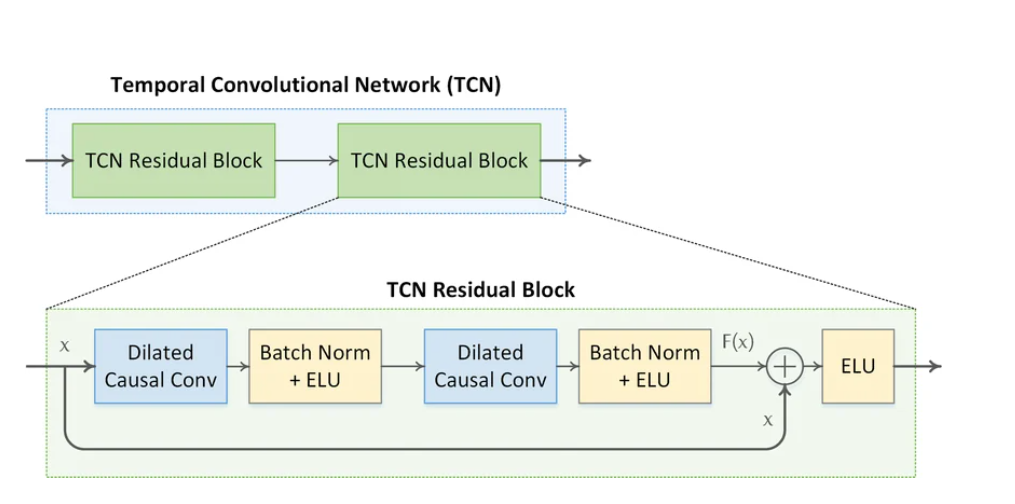
\includegraphics[width=0.8\linewidth]{image/TCN_sodo.png}
    \caption{Mô hình TCN}
    \label{fig:tcn-model}
\end{figure}

\subsubsection{Phân tích chi tiết từ hiện thực}

\begin{itemize}
    \item \textbf{Lớp TCN:} Được cấu hình với 32 bộ lọc (\texttt{nb\_filters = 32}) và kích thước nhân tích chập (\texttt{kernel\_size = 3}). Với mảng hệ số giãn cách:
    \[
    [1,\; 2,\; 4,\; 8]
    \]
    lớp này có khả năng trích xuất đặc trưng trên phạm vi thời gian rộng mà vẫn bảo toàn tính nhân quả của chuỗi dữ liệu.
    
    \item \textbf{Các lớp Dense:} Lớp ẩn với 16 nơ-ron sử dụng hàm kích hoạt ReLU giúp mô hình học được các quan hệ phi tuyến tính phức tạp giữa các thông số môi trường.
    
    \item \textbf{Kích thước mô hình:} Tổng số tham số huấn luyện là 23\,233, tương đương dung lượng khoảng 90.75 KB. Đây là kích thước rất nhỏ, phù hợp để triển khai trên Raspberry Pi 4 và đảm bảo tốc độ suy luận nhanh trong thời gian thực.
\end{itemize}

\subsection{Hiện thực Quy trình Huấn luyện và Giám sát}

Giai đoạn này tập trung vào việc hiện thực hóa quá trình huấn luyện mô hình TCN trên tập dữ liệu đã được tiền xử lý. Hệ thống được thiết kế để tự động theo dõi hiệu suất và dừng đúng thời điểm nhằm tối ưu hóa thời gian tính toán.

\subsubsection{Hiện thực cấu hình tham số huấn luyện}

Các tham số điều khiển quá trình học (\textit{hyperparameters}) được thiết lập trực tiếp trong mã nguồn \texttt{main.py} để đảm bảo tính ổn định và khả năng hội tụ của mạng nơ-ron.

\begin{itemize}
    \item \textbf{Thuật toán tối ưu (Optimizer):} Sử dụng Adam với tốc độ học (\textit{learning rate}) là $0.001$.
    
    \item \textbf{Hàm mất mát (Loss Function):} Sử dụng Mean Squared Error (MSE), đồng thời theo dõi Mean Absolute Error (MAE).
    
    \item \textbf{Kích thước lô (Batch Size):} Thiết lập bằng 32 mẫu cho mỗi lần cập nhật trọng số.
\end{itemize}

\subsubsection{Hiện thực cơ chế Giám sát và Dừng sớm (Early Stopping)}

Để ngăn chặn hiện tượng quá khớp (\textit{overfitting}) và tiết kiệm tài nguyên hệ thống, callback \texttt{EarlyStopping} được tích hợp vào quá trình huấn luyện.

\begin{lstlisting}[style=thesisstyle, language=Python]
early_stop = EarlyStopping(
    monitor='val_loss',
    patience=15,
    restore_best_weights=True
)
\end{lstlisting}

Callback này theo dõi giá trị \texttt{val\_loss}. Nếu sau 15 epoch liên tiếp không có cải thiện, quá trình huấn luyện sẽ tự động dừng và khôi phục lại bộ trọng số tốt nhất.

\subsubsection{Nhật ký thực thi quá trình huấn luyện}

Quá trình huấn luyện được khởi chạy bằng lệnh:

\begin{lstlisting}[style=thesisstyle, language=bash]
python main.py
\end{lstlisting}

Trong suốt quá trình này, hệ thống xuất ra nhật ký chi tiết cho từng epoch để theo dõi thời gian xử lý và giá trị sai số.

\begin{figure}[H]
    \centering
    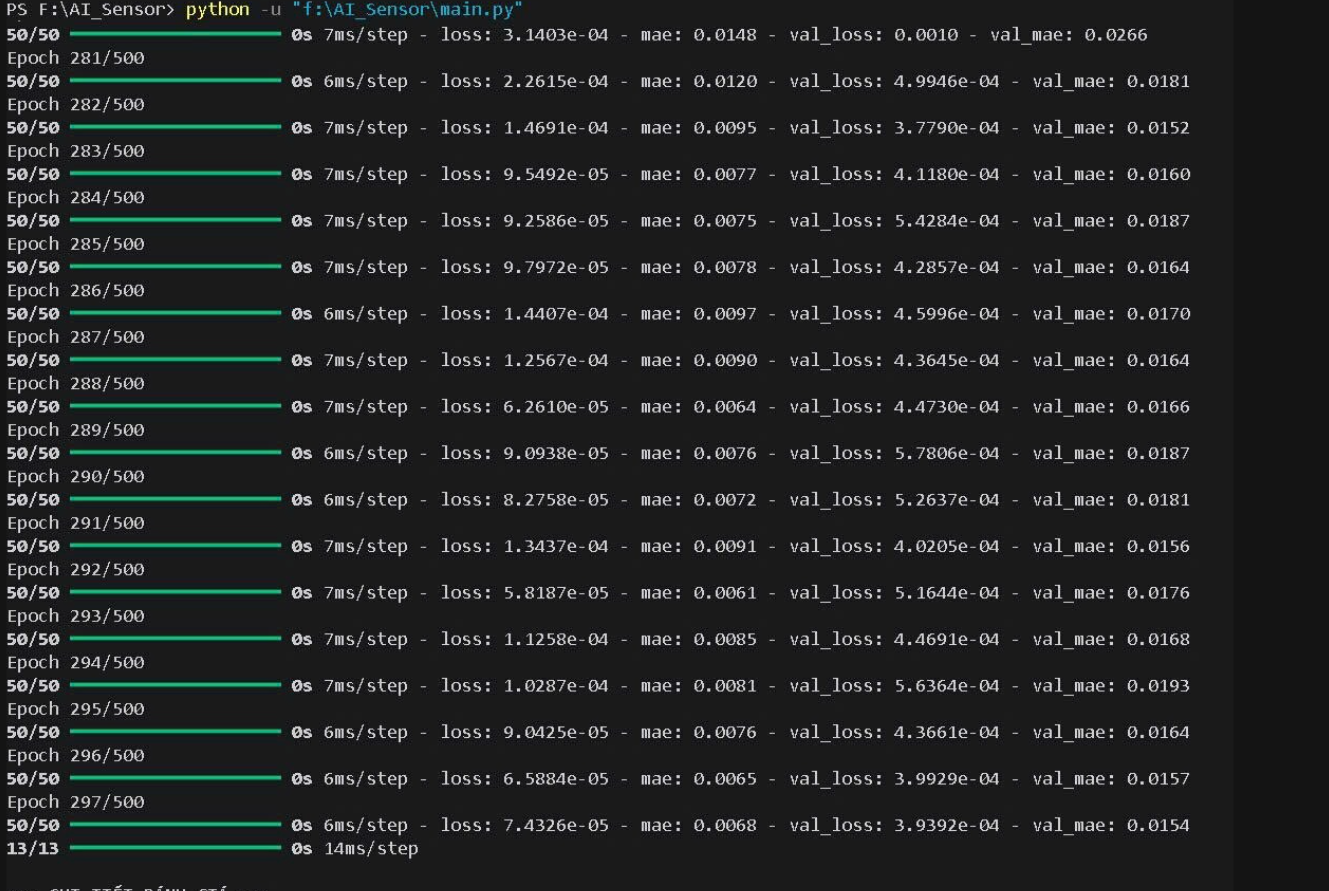
\includegraphics[width=0.7\textwidth]{image/train_quan.png}
    \caption{Nhật ký quá trình huấn luyện mô hình TCN trên môi trường máy trạm}
    \label{fig:training-log}
\end{figure}

Dựa trên nhật ký thực thi thực tế ở Hình~\ref{fig:training-log}, có thể rút ra các nhận xét sau:

\begin{itemize}
    \item \textbf{Trạng thái dừng:} Mặc dù số lượng epoch tối đa được thiết lập là 500, cơ chế Early Stopping đã tự động dừng quá trình huấn luyện tại epoch 297.
    
    \item \textbf{Hiệu suất thời gian:} Mỗi bước huấn luyện chỉ mất trung bình từ 6\,ms đến 7\,ms.
    
    \item \textbf{Đóng gói kết quả:} Sau khi huấn luyện kết thúc, mô hình được lưu vào tệp \texttt{tcn\_model.keras} để phục vụ cho bước chuyển đổi sang TensorFlow Lite.
\end{itemize}

\section{Hiện thực hệ thống cập nhập từ xa OTA}
Phần này trình bày chi tiết quá trình hiện thực hóa giải pháp cập nhật phần mềm từ xa (Over-the-Air -- OTA) cho thiết bị Raspberry Pi 4. Quá trình hiện thực bao gồm việc cấu hình môi trường build Yocto, tùy chỉnh các recipe hệ thống, xây dựng kịch bản mô tả và triển khai thực tế trên phần cứng.

\subsection{Tích hợp các Layer và Cấu hình môi trường Yocto}

Để hệ thống có khả năng xử lý OTA, bước đầu tiên là tích hợp framework SWUpdate vào quy trình xây dựng image của Yocto Project (nhánh Kirkstone).

\begin{itemize}
    \item \textbf{Quản lý Layer:} Việc tích hợp được thực hiện thông qua sửa đổi tệp \texttt{conf/bblayers.conf}. Hệ thống sử dụng layer cộng đồng \texttt{meta-swupdate} để cung cấp các công cụ lõi và layer tùy chỉnh \texttt{meta-ota} để chứa các cấu hình riêng biệt của đồ án. Cách phân tách này giúp quản lý mã nguồn dễ dàng và tránh xung đột khi cập nhật framework.

    \item \textbf{Khai báo thành phần hệ thống:} Trong tệp \texttt{conf/local.conf}, biến \texttt{IMAGE\_INSTALL:append} được khai báo để yêu cầu BitBake đóng gói các gói cần thiết vào Root File System. Các thành phần bao gồm:
    \begin{itemize}
        \item \texttt{swupdate}: chương trình chính thực hiện cập nhật.
        \item \texttt{swupdate-www}: giao diện Web UI.
        \item \texttt{libconfig}: thư viện phân tích cú pháp cho tệp \texttt{sw-description}.
        \item \texttt{u-boot-fw-utils}: công cụ giao tiếp với bootloader U-Boot.
    \end{itemize}

    \item \textbf{Tùy chỉnh Init System:} Hệ thống sử dụng \texttt{systemd} làm trình quản lý dịch vụ. Vì vậy, SWUpdate được cấu hình để hoạt động như một daemon và tự động khởi động cùng hệ thống.
\begin{lstlisting}[style=thesisstyle, language=C]
POKY_BBLAYERS_CONF_VERSION = "2"

BBPATH = "${TOPDIR}"
BBFILES ?= ""

BBLAYERS ?= " \
  /workspace/DATN-main/DATN-main/yocto/meta \
  /workspace/DATN-main/DATN-main/yocto/meta-poky \
  /workspace/DATN-main/DATN-main/yocto/meta-yocto-bsp \
  /workspace/DATN-main/layers/meta-raspberrypi \
  /workspace/DATN-main/layers/meta-openembedded/meta-oe \
  /workspace/DATN-main/layers/meta-openembedded/meta-python \
  /workspace/DATN-main/layers/meta-openembedded/meta-networking \
  /workspace/DATN-main/layers/meta-openembedded/meta-multimedia \
  /workspace/DATN-main/layers/meta-rs485 \
  /workspace/DATN-main/layers/meta-i2c \
  /workspace/DATN-main/layers/meta-qt5 \
  /workspace/DATN-main/DATN-main/yocto/build/meta-ota \
  /workspace/DATN-main/layers/meta-swupdate \
  "

\end{lstlisting}
\end{itemize}


\subsection{Hiện thực và Tùy chỉnh Recipe SWUpdate}

Hệ thống không sử dụng cấu hình mặc định mà triển khai cơ chế ghi đè (\textit{override}) thông qua tệp \texttt{swupdate\_\%.bbappend}.

\begin{itemize}
    \item \textbf{Tùy chỉnh cấu hình (Defconfig):} Thông qua lệnh:
\begin{lstlisting}[style=thesisstyle, language=bash]
bitbake swupdate -c menuconfig
\end{lstlisting}

Tùy chỉnh cấu hình (Defconfig): Thông qua lệnh bitbake swupdate -c menuconfig, hệ thống đã thực hiện tinh chỉnh các tham số quan trọng. Sau đó, tệp .config được lưu lại thành defconfig trong thư mục files của layer.

    \item \textbf{Các tùy chọn cấu hình chính:}
    \begin{itemize}
        \item \texttt{CONFIG\_LIBCONFIG=y}: Kích hoạt bộ phân tích cú pháp cho tệp \texttt{sw-description}.
        \item \texttt{CONFIG\_MONGOOSE=y}: Tích hợp máy chủ Web Mongoose vào SWUpdate để nhận gói cập nhật qua HTTP mà không cần cài thêm Nginx hoặc Apache.
        \item \texttt{CONFIG\_UBOOT=y}: Cho phép SWUpdate sử dụng thư viện \texttt{libubootenv} để ghi trực tiếp các biến môi trường của U-Boot.
    \end{itemize}

    \item \textbf{Quản lý file nguồn:} Recipe được cấu hình để bổ sung các tệp như \texttt{swupdate.service} và \texttt{hwrevision} vào thư mục \texttt{/etc/} trên Raspberry Pi 4.
\end{itemize}

    \begin{figure}[H]
    \centering
    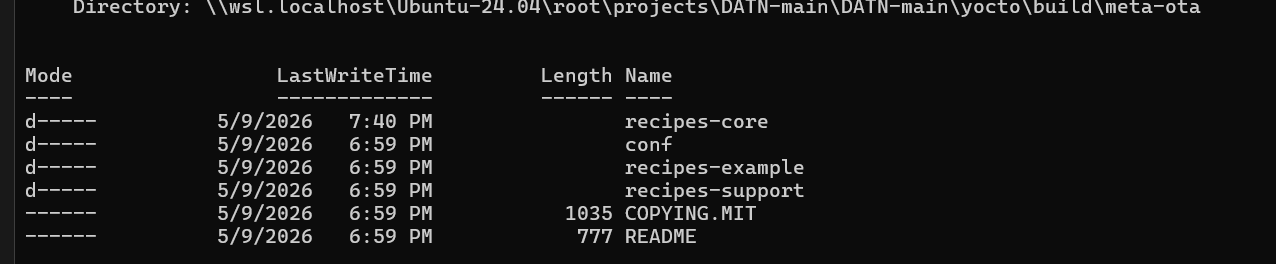
\includegraphics[width=0.7\textwidth]{image/mete-ota.png}
    \label{fig:meta-ota}
  \end{figure}
\subsection{Xây dựng Kịch bản Mô tả Hệ thống }

Tệp \texttt{sw-description} đóng vai trò là ``linh hồn'' của bản cập nhật, chứa toàn bộ thông tin định danh và chỉ thị cài đặt.

\begin{itemize}
    \item \textbf{Cấu trúc tệp:} Sử dụng định dạng Libconfig với cấu trúc phân cấp. Phần \texttt{software} định nghĩa phiên bản (ví dụ: \texttt{1.0.1}); phần \texttt{images} chứa danh sách các tệp ảnh hệ điều hành cần nạp.

    \item \textbf{Logic thực thi:} Thiết bị đích được chỉ định là \texttt{/dev/mmcblk0p3} (phân vùng dự phòng). Tham số:
\begin{lstlisting}[style=thesisstyle]
type = "raw";
\end{lstlisting}
    yêu cầu SWUpdate sử dụng cơ chế ghi dữ liệu thô theo từng sector, đảm bảo tính toàn vẹn tuyệt đối của Root File System.

    \item \textbf{Xác thực Checksum:} Mỗi mục \texttt{image} đi kèm một mã băm SHA256 để kiểm tra tính toàn vẹn dữ liệu sau khi ghi, giúp phát hiện lỗi do truyền tải mạng hoặc lỗi thiết bị lưu trữ.
\end{itemize}
\begin{lstlisting}[style=thesisstyle, language=C]
software = {
    version = "1.0.1";
    raspberrypi4-64 = {
        images: (
            {
                filename = "rootfs.ext4.gz";
                device = "/dev/mmcblk0p3"; // Phan vung dich (Slot B)
                type = "raw";
                compressed = "zlib";
                install-if-different = true;
            }
        );
        scripts: (
            {
                filename = "update_boot_env.sh";
                type = "shellscript";
            }
        );
    }
}

\end{lstlisting}
\subsection{Hiện thực Kịch bản Hậu cập nhật và Giao tiếp Bootloader}

Một trong những thách thức lớn nhất của hệ thống OTA là chuyển đổi phân vùng khởi động sau khi ghi dữ liệu thành công.

\begin{itemize}
    \item \textbf{Viết kịch bản Shell:} Hệ thống hiện thực tệp \texttt{update\_boot\_env.sh}. Tập lệnh này được SWUpdate tự động gọi sau khi quá trình ghi image hoàn tất.

    \item \textbf{Thao tác với U-Boot:} Sử dụng công cụ \texttt{fw\_setenv} để cập nhật biến môi trường của bootloader.
    \begin{itemize}
        \item \texttt{fw\_setenv ustate 1}: Đánh dấu hệ thống đang ở trạng thái cập nhật.
        \item \texttt{fw\_setenv boot\_targets mmc0:3}: Chỉ định khởi động từ phân vùng mới được cập nhật.
    \end{itemize}

    \item \textbf{Tính an toàn:} Nếu kịch bản hậu cập nhật thất bại, hệ thống sẽ không chuyển đổi slot, đảm bảo thiết bị tiếp tục khởi động vào phiên bản ổn định trước đó.
\end{itemize}

\begin{lstlisting}[style=thesisstyle, language=Python]
USTATE_INSTALLED=1
echo "--- Post-install script started ---"
echo "Setting U-Boot variable: ustate = $USTATE_INSTALLED"
fw_setenv ustate $USTATE_INSTALLED
echo "Switching boot target to Slot B..."
fw_setenv boot_slot 3
echo "--- Post-install script finished successfully ---"
exit 0
\end{lstlisting}
\subsection{Quy trình Đóng gói và Triển khai Vận hành Thực tế}

Đây là giai đoạn cuối cùng, chuyển đổi các sản phẩm từ quá trình build thành một gói cập nhật hoàn chỉnh.

\begin{itemize}
    \item \textbf{Đóng gói định dạng \texttt{.swu}:} Hệ thống sử dụng công cụ \texttt{cpio} với tùy chọn \texttt{-H crc}. Một yêu cầu bắt buộc là tệp \texttt{sw-description} phải nằm ở vị trí đầu tiên trong gói để SWUpdate có thể đọc thông tin mô tả trước khi xử lý các tệp image lớn.

    \item \textbf{Khởi chạy Daemon trên Raspberry Pi 4:}
\begin{lstlisting}[style=thesisstyle, language=bash]
swupdate -w "-r /www -p 9090"
\end{lstlisting}
    Lệnh này kích hoạt Web UI của SWUpdate tại cổng 9090.

    \item \textbf{Triển khai thực tế:} Người dùng truy cập địa chỉ IP của Raspberry Pi 4 trên cổng 9090 bằng trình duyệt. Khi tệp \texttt{.swu} được tải lên, dữ liệu sẽ được giải nén và ghi trực tiếp vào phân vùng \texttt{/dev/mmcblk0p3}. Sau khi hoàn tất, hệ thống tự động thực thi kịch bản hậu cập nhật và khởi động lại để kích hoạt phiên bản mới.
\end{itemize}

\section{Hiện thực Tool Build Yocto}

Trong quy trình phát triển hệ điều hành nhúng với Yocto Project, việc cấu hình các tệp tin \texttt{.conf} và quản lý hàng trăm lớp (\textit{layers}) metadata thường gây khó khăn và dễ dẫn đến sai sót cấu hình thủ công. Để giải quyết vấn đề này, một công cụ quản lý tập trung -- \textit{Secure-Yocto Builder} -- đã được hiện thực hóa. Công cụ này không chỉ đơn thuần là một giao diện đồ họa mà còn đóng vai trò là một lớp trung gian (\textit{Middleware}) xử lý logic nghiệp vụ, tích hợp trí tuệ nhân tạo để hỗ trợ gỡ lỗi.

\subsection{Kiến trúc phân lớp và Luồng dữ liệu}

Dựa trên sơ đồ khối hệ thống (Hình 4.5), công cụ được xây dựng theo kiến trúc 3 lớp (\textit{3-tier architecture}) nhằm đảm bảo tính module và khả năng mở rộng:

\begin{itemize}
    \item \textbf{Lớp User (Presentation Layer):} Hiện thực bằng HTML5/CSS3 và JavaScript theo phong cách Terminal User Interface (TUI). Lớp này chịu trách nhiệm thu thập thông tin cấu hình từ người dùng và hiển thị trạng thái Build theo thời gian thực.

    \item \textbf{Lớp Xử lý Logic (Business Logic Layer -- Backend):} Sử dụng framework Flask. Đây là ``bộ não'' của công cụ, thực hiện việc chuyển đổi các yêu cầu từ giao diện thành các thao tác điều chỉnh tệp tin hệ thống hoặc thực thi các lệnh Linux.

    \item \textbf{Lớp Tương tác Hệ thống (System Interaction Layer):} Bao gồm các tập lệnh Shell, công cụ BitBake của Yocto và các API bên thứ ba (Google Gemini).
\end{itemize}
\subsection{Hiện thực Lớp Backend (Flask API)}

Backend được thiết kế để xử lý các yêu cầu bất đồng bộ từ Frontend thông qua giao thức HTTP/JSON.

\subsubsection{Kỹ thuật điều khiển cấu hình bằng Biểu thức chính quy (Regex)}

Thay vì nạp toàn bộ tệp cấu hình vào bộ nhớ (có thể gây mất dữ liệu nếu tệp quá lớn), công cụ sử dụng hàm \texttt{toggle\_file\_line} để xử lý tệp tin theo từng dòng. Kỹ thuật này sử dụng Regex để tìm đúng từ khóa cấu hình và thực hiện việc comment (\texttt{\#}) hoặc uncomment dựa trên trạng thái người dùng chọn trên UI.

\begin{lstlisting}[style=thesisstyle, language=Python]
def toggle_file_line(filepath, search_pattern, enable=True):
    """
    Tu dong hoa viec cau hinh file local.conf va bblayers.conf
    """
    if not os.path.exists(filepath):
        return

    with open(filepath, 'r') as file:
        lines = file.readlines()

    with open(filepath, 'w') as file:
        for line in lines:
            # Su dung Regex de dinh vi chinh xac dong cau hinh can tac dong
            if re.search(search_pattern, line):
                if enable:
                    # Xoa ky tu comment o dau dong de kich hoat tinh nang
                    line = re.sub(r'^#\s*', '', line)
                else:
                    # Them dau comment neu nguoi dung tat tinh nang tren UI
                    if not line.startswith('#'):
                        line = f"# {line}"
            file.write(line)
\end{lstlisting}

\subsubsection{Quản lý quy trình thực thi BitBake}

Việc thực thi lệnh \texttt{bitbake} tiêu tốn rất nhiều tài nguyên và thời gian. Để tránh việc làm treo (\textit{blocking}) server Flask, công cụ sử dụng lớp \texttt{subprocess.Popen}. Toàn bộ luồng dữ liệu chuẩn (\texttt{stdout}) và luồng lỗi (\texttt{stderr}) được chuyển hướng trực tiếp ra terminal của máy chủ và đồng thời ghi vào tệp \texttt{terminal\_errors.log}.

\begin{lstlisting}[style=thesisstyle, language=Python]
@app.route('/api/start_build', methods=['POST'])
def start_build():
    # Thiet lap moi truong Yocto thong qua lenh source
    setup_env = '/workspace/DATN-main/DATN-main/yocto/oe-init-build-env'
    cmd = f"bash -c 'source {setup_env} {YOCTO_BUILD_DIR} && bitbake {image_name}' 2>&1 | tee {TERMINAL_LOG}"

    # Khoi chay tien trinh con de thuc hien build bat dong bo
    process = subprocess.Popen(
        cmd,
        shell=True,
        stdout=sys.stdout,
        stderr=sys.stderr
    )

    return jsonify({
        "status": "Success",
        "message": "Tien trinh Build da khoi dong!"
    })
\end{lstlisting}

\subsection{Hiện thực Giao diện người dùng (Frontend TUI)}

Giao diện được thiết kế để tối ưu hóa trải nghiệm cho lập trình viên hệ thống, tập trung vào sự tinh gọn và tốc độ truy cập.

\subsubsection{Quản lý trạng thái (State Management)}

Một đối tượng \texttt{state} trong JavaScript được duy trì để đồng bộ hóa các lựa chọn của người dùng (Target, Security Features, Drivers) với giao diện.

\subsubsection{Xử lý sự kiện (Event Handling)}

Khi người dùng thay đổi một tùy chọn bảo mật (như bật SELinux), một hàm \texttt{fetch} sẽ được kích hoạt để gửi tín hiệu ngay lập tức về Backend mà không cần tải lại trang.

\begin{lstlisting}[style=thesisstyle, language=Python]
async function toggleSecurityOnBackend(featureName, isChecked) {
    const featureMap = {
        'SELinux (refpolicy-mls)': 'selinux',
        'dm-verity (RootFS integrity)': 'dmverity',
        'Read-only RootFS': 'readonly'
    };

    // Gui yeu cau cap nhat file cau hinh ngay khi nguoi dung click
    await fetch('/api/toggle_security', {
        method: 'POST',
        headers: {'Content-Type': 'application/json'},
        body: JSON.stringify({
            feature: featureMap[featureName],
            value: isChecked
        })
    });
}
\end{lstlisting}

\subsection{Tích hợp các module phân tích thông minh}

\subsubsection{Module AI Debugger (Gemini Analytics)}

Khi quá trình Build gặp lỗi (\textit{Failure}), người dùng thường phải xử lý hàng nghìn dòng log phức tạp. Module \texttt{ai\_debug} được xây dựng nhằm tự động trích xuất 30 dòng lỗi cuối cùng trong tệp \texttt{terminal\_errors.log} và gửi đến mô hình Gemini 1.5 Flash để phân tích.

AI có khả năng nhận diện các lỗi phổ biến như thiếu thư viện phụ thuộc, sai cú pháp Recipe, lỗi cấu hình hoặc lỗi phân quyền truy cập. Sau khi phân tích, hệ thống sẽ trả về nguyên nhân và đề xuất hướng khắc phục bằng tiếng Việt.

Quy trình gỡ lỗi thông minh gồm các bước sau:

\begin{itemize}
    \item Trích xuất 30 dòng cuối cùng của tệp log chứa thông tin lỗi.
    \item Gửi nội dung log cùng Prompt mô tả ngữ cảnh đến Gemini 1.5 Flash.
    \item AI phân tích nguyên nhân và sinh hướng dẫn khắc phục.
    \item Kết quả được hiển thị trực tiếp trên giao diện Web.
\end{itemize}

Nhờ tích hợp AI, thời gian tìm nguyên nhân lỗi được rút ngắn đáng kể, giúp lập trình viên xử lý sự cố nhanh chóng và hiệu quả hơn.
\subsubsection{Module Quét lỗ hổng bảo mật (CVE Scan Integration)}

Đây là tính năng cốt lõi nhằm đảm bảo tính bảo mật của hệ điều hành đầu ra. Hệ thống thực thi task \texttt{cve\_check} của Yocto, sau đó Backend sẽ phân tích tệp kết quả \texttt{cve-summary.json}. Dữ liệu được phân loại theo mức độ nghiêm trọng như Critical, High và Medium, đồng thời hiển thị trực quan trên giao diện Web. Người dùng có thể nhấp vào từng mã CVE để truy cập cơ sở dữ liệu NVD (\textit{National Vulnerability Database}) và xem thông tin chi tiết.

Quy trình quét lỗ hổng được thực hiện như sau:

\begin{itemize}
    \item Yocto thực thi task \texttt{cve\_check} và sinh báo cáo \texttt{cve-summary.json}.
    \item Backend phân tích tệp JSON để trích xuất tên gói, mã CVE và mức độ nghiêm trọng.
    \item Dữ liệu được tổng hợp và hiển thị trên giao diện Web dưới dạng bảng trực quan.
    \item Người dùng có thể nhấp vào liên kết CVE để xem chi tiết trên NVD.
\end{itemize}

Tính năng này giúp lập trình viên nhanh chóng đánh giá mức độ an toàn của hệ thống và chủ động xử lý các lỗ hổng bảo mật trước khi triển khai.



\chapter{Kết luận và hướng phát triển }


\begin{enumerate}[
    leftmargin=2.5em,
    labelsep=0.8em,
    itemsep=0.6em
]
  \renewcommand{\labelenumi}{\textcolor{chaptercolor}{\bfseries \thechapter.\arabic{enumi}}}
  \item \textbf{Kết luận}
  \item \textbf{Hướng phát triển}
\end{enumerate}

\newpage

\section{Kết luận}

Trong phạm vi đề tài, hệ thống Linux Embedded dựa trên Yocto Project đã được xây dựng và triển khai thành công trên nền tảng Raspberry Pi 4. Hệ thống đáp ứng mục tiêu xây dựng một nền tảng nhúng có khả năng tùy biến cao, tích hợp driver phần cứng và các thành phần IoT phục vụ bài toán giám sát công nghiệp.

Driver RS485 Modbus RTU được hiện thực dưới dạng kernel module và đã hoạt động ổn định trong quá trình thử nghiệm. Cơ chế polling dữ liệu kết hợp Serdev và UART giúp hệ thống thu thập dữ liệu cảm biến theo thời gian thực. Dữ liệu sau khi xử lý được đồng bộ giữa Kernel Space và User Space thông qua character device.

Ở tầng ứng dụng, hệ thống đã tích hợp cơ chế truyền dữ liệu IoT thông qua MQTT, phục vụ việc giám sát từ xa. Giao diện hiển thị được xây dựng để theo dõi trực quan trạng thái hệ thống và dữ liệu cảm biến. Bên cạnh đó, hệ thống có tích hợp một mô-đun phân tích dữ liệu đơn giản (AI-based), nhằm hỗ trợ đánh giá trạng thái và đưa ra cảnh báo dựa trên dữ liệu thu thập được.

Kết quả thực nghiệm cho thấy hệ thống hoạt động ổn định trên Raspberry Pi 4, đảm bảo luồng dữ liệu từ cảm biến → xử lý → truyền IoT → hiển thị được vận hành liên tục trong môi trường Linux Embedded.

\section{Hướng phát triển}

Trong tương lai, hệ thống có thể tiếp tục được mở rộng theo hướng tối ưu hiệu năng driver và giảm độ trễ trong giao tiếp RS485, đặc biệt trong môi trường nhiều thiết bị.

Về bảo mật, các cơ chế hiện tại có thể được hoàn thiện thêm để đảm bảo an toàn toàn diện hơn, bao gồm xác thực firmware, bảo vệ filesystem và tăng cường kiểm soát truy cập hệ thống.

Đối với phần phân tích dữ liệu, mô-đun AI hiện tại có thể được mở rộng theo hướng sử dụng các mô hình học máy chuyên sâu hơn nhằm nâng cao độ chính xác trong dự đoán và phát hiện bất thường so với phương pháp ngưỡng đang sử dụng.

Cuối cùng, hệ thống IoT có thể được phát triển theo hướng kiến trúc phân tán hoặc tích hợp cloud-native để đáp ứng các bài toán giám sát có quy mô lớn trong thực tế công nghiệp.
% ===== CONFIG =====
\numberwithin{figure}{chapter}
\numberwithin{table}{chapter}

\bibliographystyle{IEEEtran}
\bibliography{references}

\end{document}